\documentclass{article}
\usepackage{amsmath}
\usepackage{amssymb}
\usepackage{enumitem}
\usepackage[utf8]{inputenc}
\usepackage{graphicx}
\usepackage{xcolor}
\usepackage{verbatim}
\usepackage{mathtools}
\graphicspath{{./} }
\usepackage{hyperref}
\usepackage[margin=1.25in]{geometry}
\pagestyle{plain}
\hypersetup{
    colorlinks,
    citecolor=black,
    filecolor=black,
    linkcolor=black,
    urlcolor=black
}

\usepackage[]{mathpazo} %Use option osf for old-style figures and small-caps; use sc for small-caps only.
\linespread{1.1538}         % Palatino needs more leading space (space between lines), and this produces a 15/11 ratio between leading space and font size.  This helps with giving inline math equations more room to breathe, and it balances out the relatively wide lines on the page.
\def\mySfFamily{\sffamily\sansmath} %Needed to turn on sans-serif math fonts locally
\renewcommand{\textsf}[1]{{\sffamily\sansmath#1}} %And a command for sans-serif text
%mathpazo somehow disables the \textsc command, so we need to bring it back.
\renewcommand{\textsc}[1]{\text{\scshape #1}}
\renewcommand{\sc}[1]{\text{\scshape #1}}
%Defining a spaced small caps font.  Needed for the running header, etc.
\newcommand{\textssc}[1]{\text{\scshape \fontfamily{ppl}\selectfont \textls[100]{\MakeLowercase{#1}}}}
\renewcommand{\sfdefault}{uop} %Uses Optima for the sans-serif font
\usepackage[T1]{fontenc}
%Getting old-style numerals
\newcommand{\oldstyle}[1]{\lowercase{\fontfamily{pplj}\selectfont #1}}
 
 % PARKER/RYAN STARTS HERE
 
\DeclarePairedDelimiter\ceil{\lceil}{\rceil}
\DeclarePairedDelimiter\floor{\lfloor}{\rfloor}
 
\newcommand{\code}[1]{{\fontfamily{pcr}\selectfont #1}}
\newcommand{\codebold}[1]{\textbf{\code{#1}}}
\newcommand*\revcomp[1]{\emph{#1}\overline{#1}}
\newcommand{\gitlogo}{
\includegraphics[height=12.5]{c0/gitlogo.png}}

% \thesubsection might use \thesection, therefore it is also redefined
\renewcommand*{\thesubsection}{\arabic{section}\Alph{subsection}}
\renewcommand{\labelitemii}{\textbullet}
\title{\Large \textbf{Problem Register for\\Bioinformatics Algorithms: An Active Learning Approach}}
\author{Parker Côté and Ryan Eveloff}
\date{}

\begin{document}
\maketitle
\begin{center}
    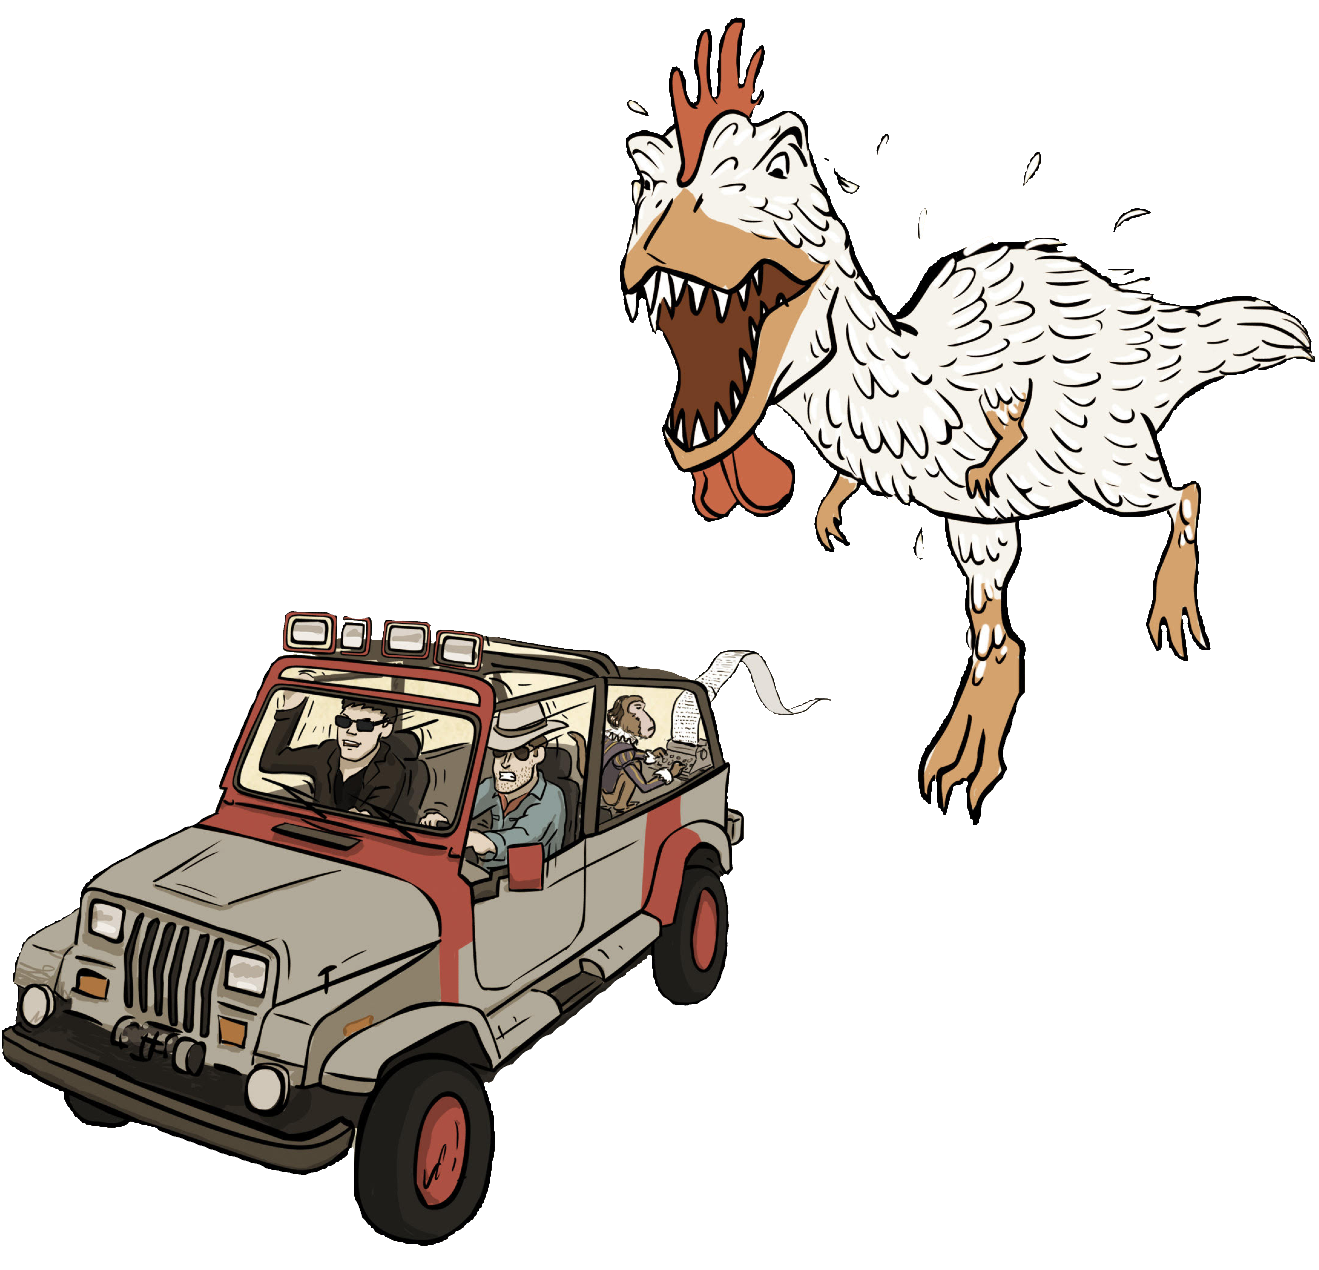
\includegraphics[scale=0.25]{c0/c0_transparent.png}
\end{center}
\pagebreak

\subsection*{Meet the Authors}
\hline\vspace{5}
\noindent\begin{minipage}{0.2\textwidth}
{%
\setlength{\fboxsep}{0pt}%
\setlength{\fboxrule}{1pt}%
\fbox{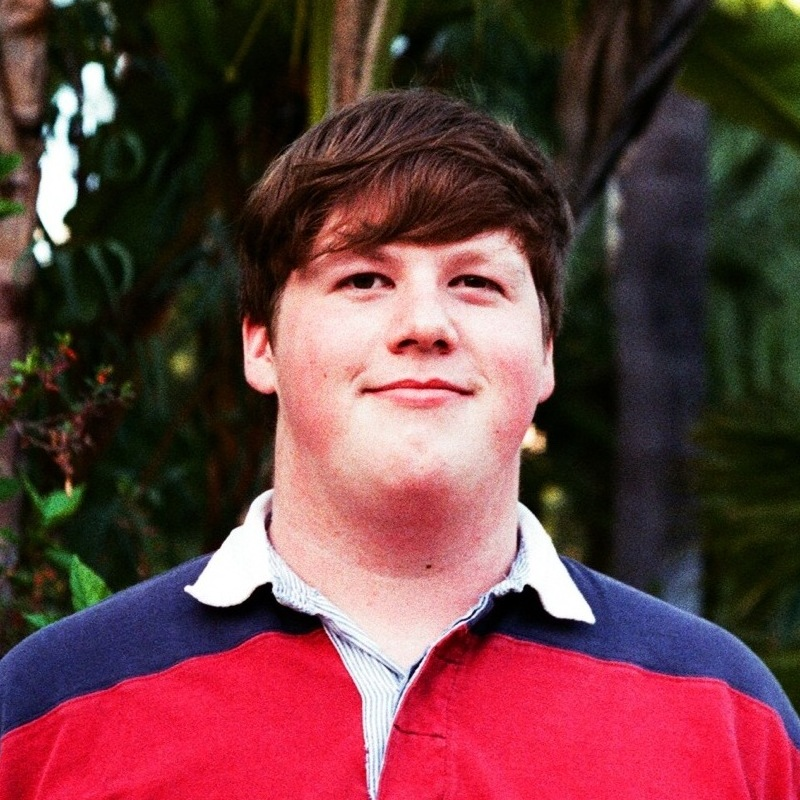
\includegraphics[width=\linewidth]{c0/Parker.jpg}}%
}%
\end{minipage}%
\hfill%
\begin{minipage}{0.75\textwidth}
\sc{Parker Côté} graduated from the Department of Biological Sciences at the University of California, San Diego in 2021 and currently works in software development at Abterra Biosciences, an antibody discovery and sequencing company based in San Diego. His research interests include precision medicine, degenerative disease, comparative genomics, and proteomics. Aside from his work in the field, he enjoys cycling, cooking, and playing music.
\end{minipage}

\vspace{32}

\noindent\begin{minipage}{0.2\textwidth}
{%
\setlength{\fboxsep}{0pt}%
\setlength{\fboxrule}{1pt}%
\fbox{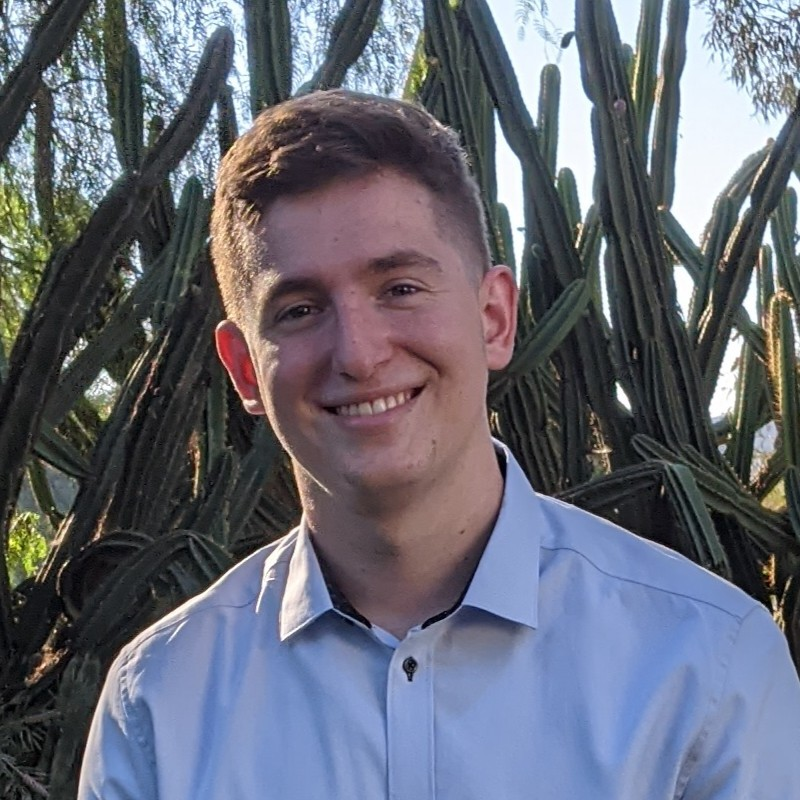
\includegraphics[width=\linewidth]{c0/Ryan.jpg}}%
}%
\end{minipage}%
\hfill%
\begin{minipage}{0.75\textwidth}
\sc{Ryan Eveloff} is a graduating senior at the University of California, San Diego in the Computer Science and Engineering department. He is particularly interested in precision medicine, neurogenetic disease, and data-informed healthcare. In 2021, he completed a joint immunology fellowship between UC San Diego and the J. Craig Venter Institute. Outside of his work, Ryan enjoys hiking around San Diego, watching college basketball, and playing electric bass.
\end{minipage}
\vspace{24} \\

\subsection*{Why We Made This}
\hline \vspace{5}

\noindent After completing Dr.~Pevzner's Bioinformatics Algorithms course at the University of California, San Diego during the Winter 2021 quarter, we came to the conclusion that a centralized, syntactically consistent register of all problems, including reproducible test cases, would have been an invaluable resource to us and our classmates. Namely, we often found ourselves stuck trying to find an edge case or confused about the parameters of a problem, but no resource existed to satisfy that need. With this problem register, we aim to fill that need.
\\
\\
Our immense thanks goes out to Dr.~Pevzner and Dr.~Compeau for giving us the opportunity to pursue this project and for offering creative directions, as well as Andrey Bzikadze and Vikram Sirupurapu for assisting in the brainstorming and proofreading processes. We hope that you can utilize this register as a resource to enrich your own learning and that of those around you. \\ \\
\noindent Best, \\
\noindent Parker $\And$ Ryan

\pagebreak

\section*{Prologue}
\subsection*{Things to know before solving Programming Challenges}
\hline\vspace{5}
\noindent Unless specified otherwise, the following are \emph{soft} rules and will not count for grading, they simply lay out the format for \emph{our} test case output.
\begin{itemize}
    \item Space separation for list elements
    \item Inputs and outputs are case sensitive
    \item When outputting integers, do not include the floating point (E.g. 1 instead of 1.0)
    \item Lexicographical ordering
\end{itemize}

\noindent Unless specified otherwise, the following are \emph{hard} rules and \emph{will} count for grading.
\begin{itemize}
    \item Zero-indexing \\
    
    \begin{center}
    \begin{tabular}{|c|c|}
    \hline
    Good     &  Bad \\ \hline
    \code{[0, 1, 2, 3][0] = 0}     & \code{[0, 1, 2, 3][1] = 0} \\
    \hline
    \end{tabular}
    \end{center}
    \item Space separation for list elements
        \begin{center}
    \begin{tabular}{|c|c|}
    \hline
    Good     &  Bad \\ \hline
    \code{0 \, 1 \, 2 \, 3}     & \code{0, 1, 2, 3} \\
    \hline
    \end{tabular}
    \end{center}
    
    \item Newline separation for arguments
    \begin{center}
    \begin{tabular}{|c|c|}
    \hline
    Good     &  Bad \\ \hline
    \code{1} & \code{1, 2} \\
    \code{2} & \\
    \hline
    \end{tabular}
    \end{center}
\end{itemize}

\subsection*{Test Cases}
\hline \vspace{5}
While we provide a range of test cases for each problems, these are \emph{not} exhaustive. We encourage you to investigate each problem to determine the potential edge cases and relevant parameters, then write your own tests as you see fit. Similarly, many of our test cases are based on the DNA alphabet (A, C, G, and T). When designing your algorithms, unless explicitly stated otherwise, you should be prepared to test on all characters, not just the characters in the genetic alphabet. Please note that the constraints provided for each question will not change and you will not be tested on datasets outside of those parameters. You should consider the effects of these constraints on runtime and memory when designing your algorithmic solutions. Lastly, you may see ellipses (\dots) in test case input/output. These are \emph{not} part of the test case and only illustrate a continuation from the previous line. \\ \\

\noindent All test cases are also available on the GitHub associated with this Problem Register. Keep an eye out for \gitlogo \, symbols that link each problem to a folder of its test cases.
\pagebreak

\tableofcontents
\newpage

\section{Where in the Genome Does DNA Replication Begin?\\ \normalfont\emph{Algorithmic Warmup}}
\begin{center}
    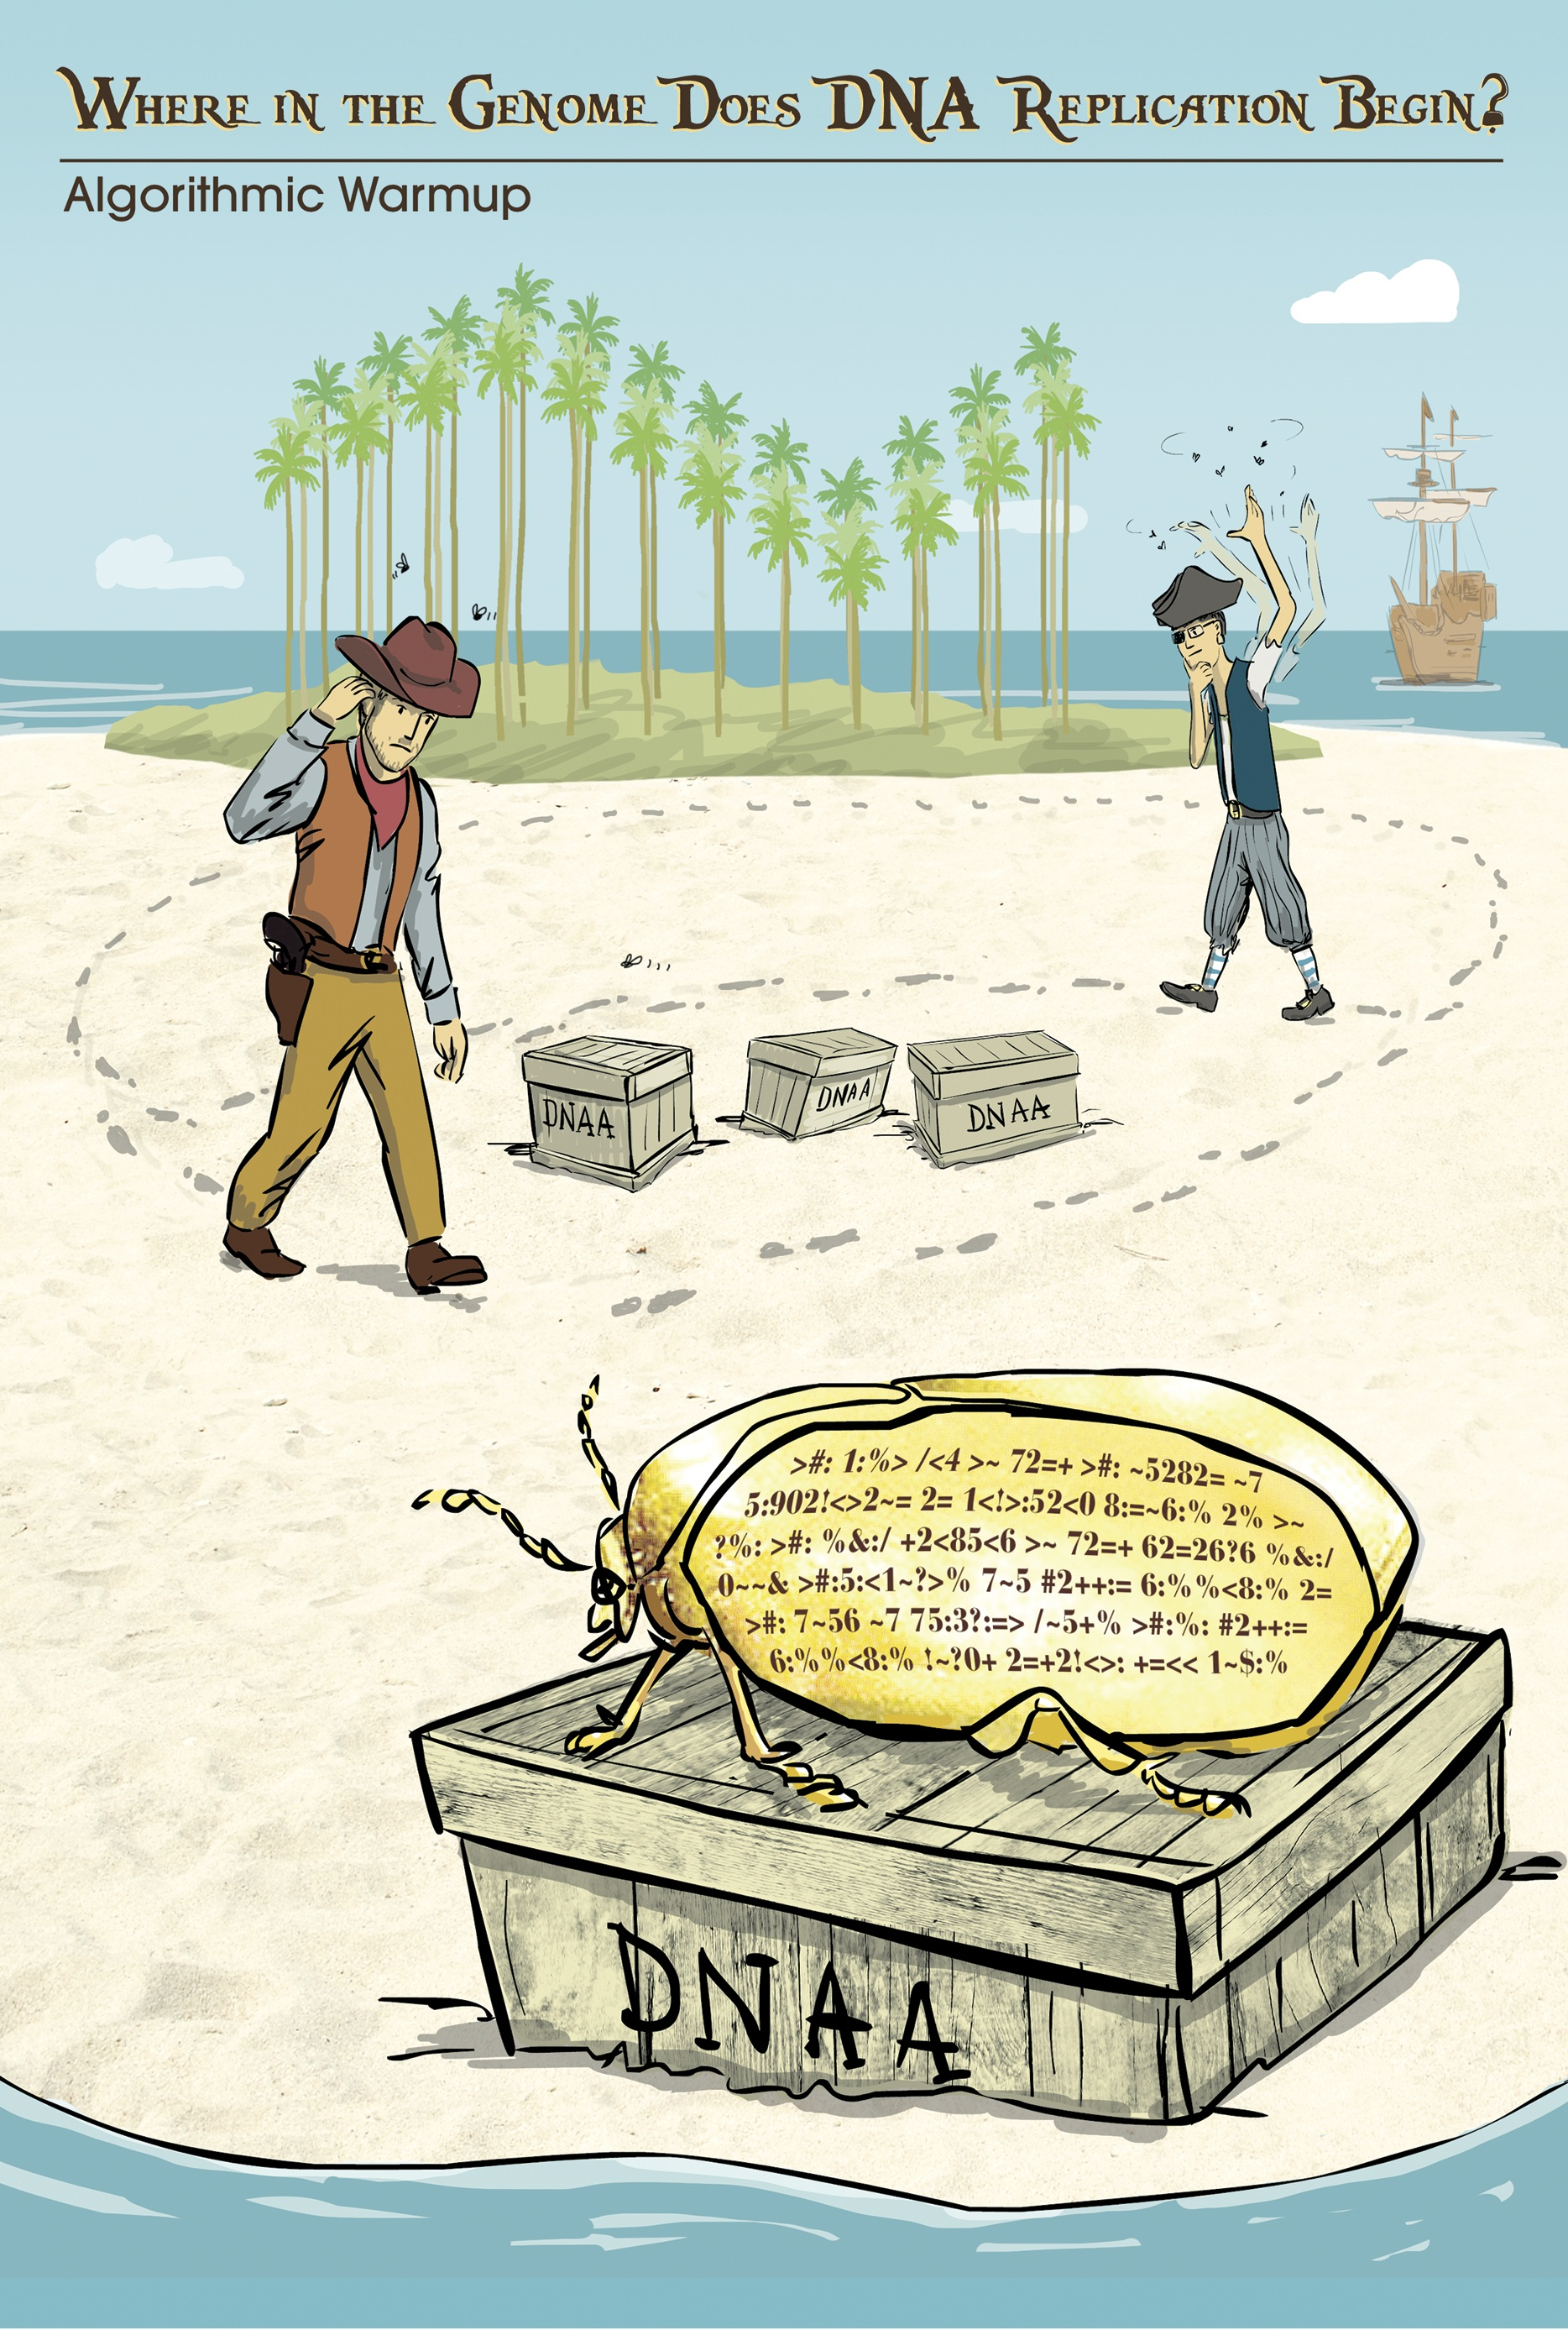
\includegraphics[scale=0.72]{c1/c1.jpg}
\end{center}
\pagebreak

\subsection{Compute the Number of Occurrences of a Pattern in a Text}
\hline\vspace{5}
\noindent \textbf{Pattern Count Problem}\\
\emph{Implement PatternCount}.\\ \\
\textbf{Input:} Strings \emph{Text} and \emph{Pattern}.\\
\textbf{Output:} The number of occurrences of \emph{Pattern} in \emph{Text}.
\begin{center}
    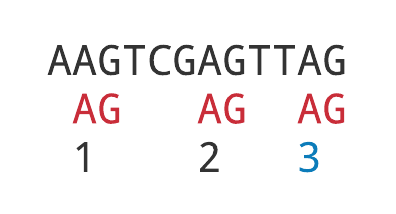
\includegraphics[scale=0.24]{c1/logos/1A.png} 
\end{center}
\hline\vspace{5}

\subsection*{Formatting}
\textbf{Input:} Newline-separated strings \emph{Text} and \emph{Pattern}.\\
\noindent \textbf{Output:} An integer representing the number of times \emph{Pattern} appears in \emph{Text}.

\subsection*{Constraints}
\begin{itemize}
    \item The length of \emph{Text} will be between $1$ and $10^4$.
    \item The length of \emph{Pattern} will be between $1$ and $10^1$.
    \item \emph{Text} and \emph{Pattern} will be DNA strings.
\end{itemize}
\pagebreak

\subsection*{\href{https://github.com/rjeveloff/BA_problemregister/tree/main/test_cases/chapter_1/1A}{Test Cases \gitlogo}}

\stepcounter{subsubsection}\subsubsection*{Case \arabic{subsubsection}}
\hline \vspace{5}
\textbf{Description:} The sample dataset is not actually run on your code. Notice that \code{GCG} occurs twice in \emph{Text}: once at the beginning (\codebold{GCG}\code{CG}) and once at the end (\code{GC}\codebold{GCG}). A common mistake for this problem is incorrectly handling overlaps and not counting the second of these two occurrences (because it begins at the end of the previous occurrence).\\ \\
\noindent \textbf{Input:}\\
\code{GCGCG \\GCG}\\ \\
\noindent \textbf{Output:}\\
\code{2}

\stepcounter{subsubsection}\subsubsection*{Case \arabic{subsubsection}}
\hline \vspace{5}
\textbf{Description:} This dataset just checks if you’re correctly counting. It is the “easiest” test. Notice that all occurrences of \code{CG} in \emph{Text} (\code{ACGTACGTACGT}) are away from the very edges (so your code won’t fail on off-by-one errors at the beginning or at the end of \emph{Text}) and that none of the occurrences of Pattern overlap (so your code won’t fail if you fail to account for overlaps).\\ \\
\noindent \textbf{Input:}\\
\code{ACGTACGTACGT\\ CG}\\ \\
\noindent \textbf{Output:}\\
\code{3}

\stepcounter{subsubsection}\subsubsection*{Case \arabic{subsubsection}}
\hline \vspace{5}
\textbf{Description:} This dataset checks if your code correctly handles cases where there is an occurrence of \emph{Pattern} at the very beginning of \emph{Text}. Note that there are no overlapping occurrences of \emph{Pattern} (i.e. \code{AAAA}), and there is no occurrence of Pattern at the very end of \emph{Text}, so assuming your code passed Test Dataset 1, this test would only check for off-by-one errors at the beginning of \emph{Text}.\\ \\
\noindent \textbf{Input:}\\
\code{AAAGAGTGTCTGATAGCAGCTTCTGAACTGGTTACCTGCCGTGAGTAAATTAAATTTTATTGACTTAGG\dots\\ \dots TCACTAAATACTTTAACCAATATAGGCATAGCGCACAGACAATAATAATTACAGAGTACACAACATCCA\\ AAA}\\ \\
\noindent \textbf{Output:}\\
\code{3}
\pagebreak

\stepcounter{subsubsection}\subsubsection*{Case \arabic{subsubsection}}
\hline \vspace{5}
\textbf{Description:} This dataset checks if your code correctly handles cases where there is an occurrence of \emph{Pattern} at the very end of \emph{Text}. Note that there are no overlapping occurrences of \emph{Pattern} (i.e. \code{AAAA}), and there is no occurrence of \emph{Pattern} at the very beginning of \emph{Text}, so assuming your code passed Test Dataset 2, this test would only check for off-by-one errors at the end of \emph{Text}.\\ \\
\noindent \textbf{Input:}\\
\code{AGCGTGCCGAAATATGCCGCCAGACCTGCTGCGGTGGCCTCGCCGACTTCACGGATGCCAAGTGCATAG\dots\\
\dots AGGAAGCGAGCAAAGGTGGTTTCTTTCGCTTTATCCAGCGCTTAACCACGTTCTGTGCCGACTTT\\ TTT}\\ \\
\noindent \textbf{Output:}\\
\code{4}

\stepcounter{subsubsection}\subsubsection*{Case \arabic{subsubsection}}
\hline \vspace{5}
\textbf{Description:} This test dataset checks if your code is also counting occurrences of the Reverse Complement of \emph{Pattern} (which would have an output of \code{4}), which is out of the scope of this problem (that will come up later in the chapter). Your code should only be looking for perfect matches of \emph{Pattern} in \emph{Text} at this point.\\ \\
\noindent \textbf{Input:}\\
\code{GGACTTACTGACGTACG\\ACT}\\ \\
\noindent \textbf{Output:}\\
\code{2}

\stepcounter{subsubsection}\subsubsection*{Case \arabic{subsubsection}}
\hline \vspace{5}
\textbf{Description:} This dataset checks if your code correctly handles cases where occurrences of \emph{Pattern}
overlap. For example, any occurrence of the string \code{CCC} should count as \code{2} occurrences of
\code{CC} (\codebold{CC}\code{C} and \code{C}\codebold{CC}). In this dataset, there are \code{5} occurrences of \code{CC} including overlaps. (\code{AT}\codebold{CC}\code{GAT}\codebold{CCC}\code{ATG}\codebold{CCC}\code{A\\TG})\\ \\
\noindent \textbf{Input:}\\
\code{ATCCGATCCCATGCCCATG\\CC}\\ \\
\noindent \textbf{Output:}\\
\code{5}
\pagebreak

\stepcounter{subsubsection}\subsubsection*{Case \arabic{subsubsection}}
\hline \vspace{5}
\textbf{Description:} This is the final test that we run your code on: the full dataset.\\ \\
\noindent \textbf{Input:}\\
\code{CTGTTTTTGATCCATGATATGTTATCTCTCCGTCATCAGAAGAACAGTGACGGATCGCCCTCTCTCTTG\dots\\
\dots GTCAGGCGACCGTTTGCCATAATGCCCATGCTTTCCAGCCAGCTCTCAAACTCCGGTGACTCGCGC\dots\\
\dots AGGTTGAGT\\CTC}\\ \\
\noindent \textbf{Output:}\\
\code{9}

\stepcounter{subsubsection}\subsubsection*{Case \arabic{subsubsection}}
\hline \vspace{5}
\textbf{Description:} A larger dataset of the same size as that provided by the randomized autograder. Check input/output folders for this dataset.\\ \\
\pagebreak
%                                                                                                                           PROBLEM BREAK
\subsection{Find the Most Frequent Words in a String}
\hline\vspace{5}
\noindent \textbf{Frequent Words Problem}\\
\emph{Find the most frequent words $k$-mers in a string}.\\ \\
\textbf{Input:} A DNA string \emph{Text} and an integer $k$.\\
\textbf{Output:} All most frequent $k$-mers in \emph{Text} (in any order).
\begin{center}
    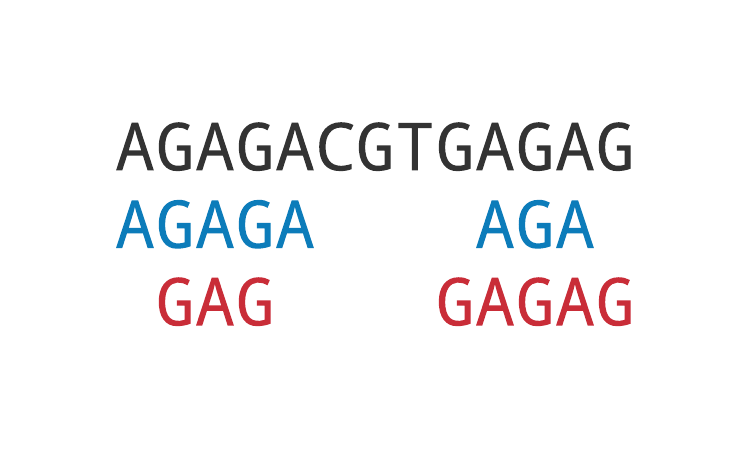
\includegraphics[scale=0.24]{c1/logos/1B.png} 
\end{center}
\hline\vspace{5}

\subsection*{Formatting}
\textbf{Input:} A DNA string \emph{Text} followed by an integer $k$.\\
\noindent \textbf{Output:} All most frequent $k$-mers in \emph{Text} (in any order).

\subsection*{Constraints}
\begin{itemize}
    \item The length of \emph{Text} will be between $1$ and $10^4$.
    \item The integer $k$ will be between $1$ and $10^2$.
    \item \emph{Text} will be a DNA string.
\end{itemize}
\pagebreak

\subsection*{\href{https://github.com/rjeveloff/BA_problemregister/tree/main/test_cases/chapter_1/1B}{Test Cases \gitlogo}}
\stepcounter{subsubsection}\subsubsection*{Case \arabic{subsubsection}}
\hline \vspace{5}
\textbf{Description:} The sample dataset is not actually run on your code.\\ \\
\noindent \textbf{Input:}\\
\code{ACGTTGCATGTCGCATGATGCATGAGAGCT\\4}\\ \\
\noindent \textbf{Output:}\\
\code{CATG GCAT}\\ \\

\stepcounter{subsubsection}\subsubsection*{Case \arabic{subsubsection}}
\hline \vspace{5}
\textbf{Description:} This dataset just checks if you’re counting the first $k$-mer in \emph{Text} (\code{TGG} in this example). If you do not count the first $k$-mer (\code{TGG}), you will get the following “most frequent” $k$-mers in addition to \code{TGG}: \code{ACT}, \code{CAC}, \code{CCA}, \code{CTT}, \code{GGT}.\\ \\
\noindent \textbf{Input:}\\
\code{TGGTAGCGACGTTGGTCCCGCCGCTTGAGAATCTGGATGAACATAAGCTCCCACTTGGCTTATTCAGAG\dots\\
\dots AACTGGTCAACACTTGTCTCTCCCAGCCAGGTCTGACCACCGGGCAACTTTTAGAGCACTATCGTG\dots\\
\dots GTACAAATAATGCTGCCAC\\3}\\ \\
\noindent \textbf{Output:}\\
\code{TGG}

\stepcounter{subsubsection}\subsubsection*{Case \arabic{subsubsection}}
\hline \vspace{5}
\textbf{Description:} This dataset just checks if you’re counting the last $k$-mer in \emph{Text} (\code{TTTT} in this example). If you do not count the last $k$-mer (\code{TTTT}), you will get the following “most frequent” $k$-mers in addition to \code{TTTT}: \code{AACG}, \code{AATA}, \code{ACAA}, \code{CAAC}, \code{CTGG}, \code{CTGG}, \code{CTTT}, \code{TTGC}, \code{TTTG}.\\ \\
\noindent \textbf{Input:}\\
\code{CAGTGGCAGATGACATTTTGCTGGTCGACTGGTTACAACAACGCCTGGGGCTTTTGAGCAACGAGACTTT\dots\\
\dots TCAATGTTGCACCGTTTGCTGCATGATATTGAAAACAATATCACCAAATAAATAACGCCTTAGTAAG\dots\\
\dots TAGCTTTT\\4}\\ \\
\noindent \textbf{Output:}\\
\code{TTTT}
\pagebreak

\stepcounter{subsubsection}\subsubsection*{Case \arabic{subsubsection}}
\hline \vspace{5}
\textbf{Description:} This dataset checks if your code correctly handles cases where there are overlapping occurrences of \emph{Pattern} throughout \emph{Text}. For example, \code{AACAACAA} contains two occurrences of \code{AACAA} (\codebold{AACAA}\code{CAA} and \code{AAC}\codebold{AACAA}), so if your code counts \code{AACAACAA} as one occurrence of \code{AACAA}, your code will fail on this test case.\\ \\
\noindent \textbf{Input:}\\
\code{ATACAATTACAGTCTGGAACCGGATGAACTGGCCGCAGGTTAACAACAGAGTTGCCAGGCACTGCCGCTG\dots\\
\dots ACCAGCAACAACAACAATGACTTTGACGCGAAGGGGATGGCATGAGCGAACTGATCGTCAGCCGTCA\dots\\
\dots GCAACGAGTATTGTTGCTGACCCTTAACAATCCCGCCGCACGTAATGCGCTAACTAATGCCCTGCTG\\5}\\ \\
\noindent \textbf{Output:}\\
\code{AACAA}

\stepcounter{subsubsection}\subsubsection*{Case \arabic{subsubsection}}
\hline \vspace{5}
\textbf{Description:} This test dataset checks if your code correctly handles ties (i.e. your code actually outputs
ALL “most frequent” $k$-mers, and not just a single “most frequent” $k$-mer). For example, in the string \code{ATATA}, there are two “most frequent” $k$-mers: \code{AT} and \code{TA}. \code{AT} occurs twice (\codebold{ATAT}\code{A}), and \code{TA} occurs twice (\code{A}\codebold{TATA}), so both of these should be output (separated by a space character).\\ \\
\noindent \textbf{Input:}\\
\code{CCAGCGGGGGTTGATGCTCTGGGGGTCACAAGATTGCATTTTTATGGGGTTGCAAAAATGTTTTTTACGG\dots\\
\dots CAGATTCATTTAAAATGCCCACTGGCTGGAGACATAGCCCGGATGCGCGTCTTTTACAACGTATTGC\dots\\
\dots GGGGTAAAATCGTAGATGTTTTAAAATAGGCGTAAC\\5}\\ \\
\noindent \textbf{Output:}\\
\code{AAAAT GGGGT TTTTA}

\stepcounter{subsubsection}\subsubsection*{Case \arabic{subsubsection}}
\hline \vspace{5}
\textbf{Description:} A larger dataset of the same size as that provided by the randomized autograder. Check input/output folders for this dataset.\\ \\
\pagebreak
%                                                                                                                           PROBLEM BREAK
\subsection{Find the Reverse Complement of a String}
\hline\vspace{5}
\noindent \textbf{Reverse Complement Problem}\\
\emph{Find the reverse complement of a DNA string}.\\ \\
\textbf{Input:} A DNA string \emph{Pattern}.\\
\textbf{Output:} The reverse complement of the string \emph{Pattern}.
\begin{center}
    
\includegraphics[scale=0.24]{c1/logos/1C.png} 
\end{center}
\hline\vspace{5}

\subsection*{Formatting}
\textbf{Input:} A DNA string \emph{Pattern}.\\
\noindent \textbf{Output:} A string representing $\overline{Pattern}$, the reverse complement of \emph{Pattern}.

\subsection*{Constraints}
\begin{itemize}
    \item The length of \emph{Pattern} will be between $1$ and $10^4$.
    \item \emph{Pattern} will be a DNA string.
\end{itemize}
\pagebreak

\subsection*{\href{https://github.com/rjeveloff/BA_problemregister/tree/main/test_cases/chapter_1/1C}{Test Cases \gitlogo}}
\stepcounter{subsubsection}\subsubsection*{Case \arabic{subsubsection}}
\hline \vspace{5}
\textbf{Description:} The sample dataset is not actually run on your code.\\ \\
\noindent \textbf{Input:}\\
\code{AAAACCCGGT}\\ \\
\noindent \textbf{Output:}\\
\code{ACCGGGTTTT}\\ \\

\stepcounter{subsubsection}\subsubsection*{Case \arabic{subsubsection}}
\hline \vspace{5}
\textbf{Description:} This test dataset performs two checks. First, it makes sure that you didn’t forget to complement \emph{Pattern} (i.e. you reversed \emph{Pattern}, but not complemented), which would have an
output of \code{CACACA}. Then, it makes sure that you didn’t forget to reverse \emph{Pattern} (i.e. you
complemented \emph{Pattern}, but not reversed), which would have an output of \code{TGTGTG}.\\ \\
\noindent \textbf{Input:}\\
\code{ACACAC}\\ \\
\noindent \textbf{Output:}\\
\code{GTGTGT}

\stepcounter{subsubsection}\subsubsection*{Case \arabic{subsubsection}}
\hline \vspace{5}
\textbf{Description:} A larger dataset of the same size as that provided by the randomized autograder. Check input/output folders for this dataset.\\ \\
\pagebreak
%                                                                                                                           PROBLEM BREAK
\subsection{Find All Occurrences of a Pattern in a String}
\hline\vspace{5}
\noindent \textbf{Pattern Matching Problem}\\
\emph{Find all occurrences of a Pattern in a string}.\\ \\
\textbf{Input:} DNA strings \emph{Pattern} and \emph{Genome}.\\
\textbf{Output:} All starting positions in \emph{Genome} where \emph{Pattern} appears as a substring.
\begin{center}
    
\includegraphics[scale=0.24]{c1/logos/1D.png} 
\end{center}
\hline\vspace{5}

\subsection*{Formatting}
\textbf{Input:} DNA strings \emph{Pattern} and \emph{Genome}.\\
\noindent \textbf{Output:} A space-separated list of integers representing each starting position in \emph{Genome} where \emph{Pattern} appears as a substring.

\subsection*{Constraints}
\begin{itemize}
    \item The length of \emph{Pattern} will be between $1$ and $10^1$.
    \item The length of \emph{Genome} will be between $1$ and $10^4$.
    \item \emph{Pattern} and \emph{Genome} will be DNA strings.
\end{itemize}
\pagebreak

\subsection*{\href{https://github.com/rjeveloff/BA_problemregister/tree/main/test_cases/chapter_1/1D}{Test Cases \gitlogo}}
\stepcounter{subsubsection}\subsubsection*{Case \arabic{subsubsection}}
\hline \vspace{5}
\textbf{Description:} The sample dataset is not actually run on your code..\\ \\
\noindent \textbf{Input:}\\
\code{ATAT\\GATATATGCATATACTT}\\ \\
\noindent \textbf{Output:}\\
\code{1 3 9}\\ \\

\stepcounter{subsubsection}\subsubsection*{Case \arabic{subsubsection}}
\hline \vspace{5}
\textbf{Description:} This dataset checks if your code is written correctly but is also taking into account reverse complements, which we are not yet doing. Even though the reverse complement of \code{ACAC} (which is \code{GTGT}) occurs in \emph{Genome}, we only want to count occurrences of \code{ACAC} specifically, which only occurs at index \code{4}.\\ \\
\noindent \textbf{Input:}\\
\code{ACAC\\TTTTACACTTTTTTGTGTAAAAA}\\ \\
\noindent \textbf{Output:}\\
\code{4}

\stepcounter{subsubsection}\subsubsection*{Case \arabic{subsubsection}}
\hline \vspace{5}
\textbf{Description:} This dataset checks for off-by-one errors at the beginning of \emph{Genome}. Notice that \code{AAA} occurs at the very beginning of \emph{Genome}, so if you were to miss the first $k$-mer of \emph{Genome}, your code would output the following: \code{46 51 74}.\\ \\
\noindent \textbf{Input:}\\
\code{AAA\\AAAGAGTGTCTGATAGCAGCTTCTGAACTGGTTACCTGCCGTGAGTAAATTAAATTTTATTGACTTAGGT\dots\\
\dots CACTAAATACTTTAACCAATATAGGCATAGCGCACAGACAGATAATAATTACAGAGTACACAACATCCAT}\\ \\
\noindent \textbf{Output:}\\
\code{0 46 51 74}
\pagebreak

\stepcounter{subsubsection}\subsubsection*{Case \arabic{subsubsection}}
\hline \vspace{5}
\textbf{Description:} This dataset checks for off-by-one errors at the end of \emph{Genome}. Notice that \code{TTT} occurs at the very end of \emph{Genome}, so if you were to miss the last $k$-mer of \emph{Genome}, your code would output the following: \code{88 93 98}.\\ \\
\noindent \textbf{Input:}\\
\code{TTT\\AGCGTGCCGAAATATGCCGCCAGACCTGCTGCGGTGGCCTCGCCGACTTCACGGATGCCAAGTGCATAGA\dots\\
\dots GGAAGCGAGCAAAGGTGGTTTCTTTCGCTTTATCCAGCGCGTTAACCACGTTCTGTGCCGACTTT}\\ \\
\noindent \textbf{Output:}\\
\code{88 92 98 132}

\stepcounter{subsubsection}\subsubsection*{Case \arabic{subsubsection}}
\hline \vspace{5}
\textbf{Description:} This test dataset checks if your code correctly handles cases where instances of \emph{Pattern} overlap in \emph{Genome}. In this case, if you did not count overlaps, you would only find the first and last instances of \code{ATA} (\codebold{ATA}\code{TATA} and \code{ATAT}\codebold{ATA}). However, there is indeed a third
occurrence, where the other two overlap (\code{AT}\codebold{ATA}\code{TA}).\\ \\
\noindent \textbf{Input:}\\
\code{ATA\\ATATATA}\\ \\
\noindent \textbf{Output:}\\
\code{0 2 4}

\stepcounter{subsubsection}\subsubsection*{Case \arabic{subsubsection}}
\hline \vspace{5}
\textbf{Description:} A larger dataset of the same size as that provided by the randomized autograder. Check input/output folders for this dataset.\\ \\
\pagebreak
%                                                                                                                           PROBLEM BREAK
\subsection{Find Patterns Forming Clumps in a String}
\hline\vspace{5}
\noindent \textbf{Clump Finding Problem}\\
\emph{Find patterns forming clumps in a string}.\\ \\
\textbf{Input:} A DNA string \emph{Genome}, and integers $k$, $L$, and $t$.\\
\textbf{Output:} All distinct $k$-mers forming ($L$, $t$)-clumps in \emph{Genome}.
\begin{center}
    
\includegraphics[scale=0.2]{c1/logos/1E.png} 
\end{center}
\hline\vspace{5}

\subsection*{Formatting}
\textbf{Input:} A DNA string \emph{Genome} followed by space-separated integers $k$, $L$, and $t$.\\
\noindent \textbf{Output:} A space-separated list of strings containing all distinct $k$-mers forming ($L$, $t$)-clumps in \emph{Genome}.

\subsection*{Constraints}
\begin{itemize}
    \item The length of \emph{Genome} will be between $1$ and $10^4$.
    \item The integer $k$ will be between $1$ and $10^1$.
    \item The integer $L$ will be between $1$ and $10^3$.
    \item The integer $t$ will be between $1$ and $10^2$.
    \item \emph{Genome} will be a DNA string.
\end{itemize}
\pagebreak

\subsection*{\href{https://github.com/rjeveloff/BA_problemregister/tree/main/test_cases/chapter_1/1E}{Test Cases \gitlogo}}
\stepcounter{subsubsection}\subsubsection*{Case \arabic{subsubsection}}
\hline \vspace{5}
\textbf{Description:} The sample dataset is not actually run on your code.\\ \\
\noindent \textbf{Input:}\\
\code{CGGACTCGACAGATGTGAAGAAATGTGAAGACTGAGTGAAGAGAAGAGGAAACACGACACGACATTGCGA\dots\\
\dots CATAATGTACGAATGTAATGTGCCTATGGC\\5 75 4}\\ \\
\noindent \textbf{Output:}\\
\code{CGACA GAAGA AATGT}

\stepcounter{subsubsection}\subsubsection*{Case \arabic{subsubsection}}
\hline \vspace{5}
\textbf{Description:} This dataset makes sure that your code only counts $k$-mers that fall \emph{completely} within a given $L$-window. For example, take the $4$-window starting at index $4$ (\code{AAAACGTCGAAAAA}). One might think that the $2$-mer \code{CG} occurs twice in this window since the first letter of the second occurrence happens at the very end of the window. However, since the second occurrence of \code{CG} does not fall entirely in this $4$-window, it does not count. Thus, the only result is \code{AA}.\\ \\
\noindent \textbf{Input:}\\
\code{AAAACGTCGAAAAA\\2 4 2}\\ \\
\noindent \textbf{Output:}\\
\code{AA}

\stepcounter{subsubsection}\subsubsection*{Case \arabic{subsubsection}}
\hline \vspace{5}
\textbf{Description:} This dataset checks if your code has an off-by-one error when checking $k$-mers within an
$L$-window. Notice that, for each $1$-mer (\code{A}, \code{C}, \code{G}, and \code{T}), there are $3$ nucleotides between the first and second occurrence. In other words, each nucleotide occurs twice in a specific $5$-window: once at the beginning of the $5$-window, and once at the end: \codebold{A}\code{CGT}\codebold{A}\code{CGT} \code{A}\codebold{C}\code{GTA}\codebold{C}\code{GT} \code{AC}\codebold{G}\code{TAC}\codebold{G}\code{T} \code{ACG}\codebold{T}\code{ACG}\codebold{T}.\\ \\
\noindent \textbf{Input:}\\
\code{ACGTACGT\\1 5 2}\\ \\
\noindent \textbf{Output:}\\
\code{A C G T}
\pagebreak

\stepcounter{subsubsection}\subsubsection*{Case \arabic{subsubsection}}
\hline \vspace{5}
\textbf{Description:} This dataset checks if your code is correctly handling overlapping $k$-mers. For example,
\code{ATA} forms a ($5$, $2$)-clump in \code{CCCATATACCC} (\code{CCC}\codebold{ATATA}\code{CCC} and \code{CCCAT}\codebold{ATACC}\code{C}).\\ \\
\noindent \textbf{Input:}\\
\code{CCACGCGGTGTACGCTGCAAAAAGCCTTGCTGAATCAAATAAGGTTCCAGCACATCCTCAATGGTTTCAC\dots\\
\dots GTTCTTCGCCAATGGCTGCCGCCAGGTTATCCAGACCTACAGGTCCACCAAAGAACTTATCGATTAC\dots\\
\dots CGCCAGCAACAATTTGCGGTCCATATAATCGAAACCTTCAGCATCGACATTCAACATATCCAGCG\\3 25 3}\\ \\
\noindent \textbf{Output:}\\
\code{AAA CAG CAT GCC TTC}

\stepcounter{subsubsection}\subsubsection*{Case \arabic{subsubsection}}
\hline \vspace{5}
\textbf{Description:} A larger dataset of the same size as that provided by the randomized autograder. Check input/output folders for this dataset.\\ \\
\pagebreak
%                                                                                                                           PROBLEM BREAK
\subsection{Find a Position in a Genome Minimizing the Skew}
\hline\vspace{5}
\noindent \textbf{Minimum Skew Problem}\\
\emph{Find a position in a genome minimizing the skew}.\\ \\
\textbf{Input:} A DNA string \emph{Genome}.\\
\textbf{Output:} All integers $i$ minimizing \sc{Skew}(\sc{Prefix}$_i$(\emph{Genome})) over all values of $i$ (from 0 to $|$\emph{Genome}$|$).
\begin{center}
    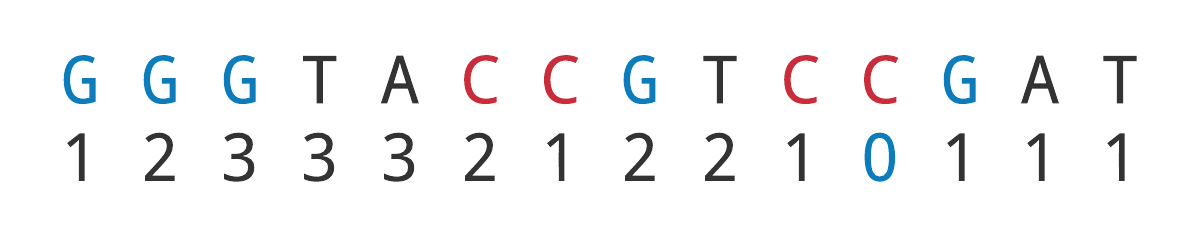
\includegraphics[scale=0.12]{c1/logos/1F.png} 
\end{center}
\hline\vspace{5}

\subsection*{Formatting}
\textbf{Input:} A DNA string \emph{Genome}.\\
\noindent \textbf{Output:} A space-separated list of integers $i$ minimizing \sc{Skew}(\sc{Prefix}$_i$(\emph{Genome}) over all values of $i$ (from 0 to $|$\emph{Genome}$|$).

\subsection*{Constraints}
\begin{itemize}
    \item The length of \emph{Genome} will be between $1$ and $10^5$.
    \item \emph{Genome} will be a DNA string.
\end{itemize}
\pagebreak

\subsection*{\href{https://github.com/rjeveloff/BA_problemregister/tree/main/test_cases/chapter_1/1F}{Test Cases \gitlogo}}
\stepcounter{subsubsection}\subsubsection*{Case \arabic{subsubsection}}
\hline \vspace{5}
\textbf{Description:} The sample dataset is not actually run on your code.\\ \\
\noindent \textbf{Input:}\\
\code{TAAAGACTGCCGAGAGGCCAACACGAGTGCTAGAACGAGGGGCGTAAACGCGGGTCCGAT}\\ \\
\noindent \textbf{Output:}\\
\code{11 24}

\stepcounter{subsubsection}\subsubsection*{Case \arabic{subsubsection}}
\hline \vspace{5}
\textbf{Description:} This dataset checks if your code’s indexing is off. Specifically, it verifies that your code
is not returning an index $1$ too high (i.e. $4$) or $1$ too low (i.e. $2$).\\ \\
\noindent \textbf{Input:}\\
\code{ACCG}\\ \\
\noindent \textbf{Output:}\\
\code{3}

\stepcounter{subsubsection}\subsubsection*{Case \arabic{subsubsection}}
\hline \vspace{5}
\textbf{Description:} This dataset checks to see if your code is missing the last symbol of \emph{Genome}.\\ \\
\noindent \textbf{Input:}\\
\code{ACCC}\\ \\
\noindent \textbf{Output:}\\
\code{4}

\stepcounter{subsubsection}\subsubsection*{Case \arabic{subsubsection}}
\hline \vspace{5}
\textbf{Description:} This dataset makes sure you’re not accidentally finding the maximum skew instead of the
minimum skew.\\ \\
\noindent \textbf{Input:}\\
\code{CCGGGT}\\ \\
\noindent \textbf{Output:}\\
\code{2}
\pagebreak

\stepcounter{subsubsection}\subsubsection*{Case \arabic{subsubsection}}
\hline \vspace{5}
\textbf{Description:} First, this dataset checks if you are only finding $1$ index (and not multiple indices). Then,
it checks if you are using a delimiter to separate your indices (a space character).\\ \\
\noindent \textbf{Input:}\\
\code{CCGGCCGG}\\ \\
\noindent \textbf{Output:}\\
\code{2 6}

\stepcounter{subsubsection}\subsubsection*{Case \arabic{subsubsection}}
\hline \vspace{5}
\textbf{Description:} A larger dataset of the same size as that provided by the randomized autograder. Check input/output folders for this dataset.\\ \\
\pagebreak
%                                                                                                                           PROBLEM BREAK
\subsection{Compute the Hamming Distance Between Two Strings}
\hline\vspace{5}
\noindent \textbf{Hamming Distance Problem}\\
\emph{Compute the Hamming distance between two strings}.\\ \\
\textbf{Input:} Two strings of equal length.\\
\textbf{Output:} The Hamming distance between these strings.
\begin{center}
    
\includegraphics[scale=0.24]{c1/logos/1G.png} 
\end{center}
\hline\vspace{5}

\subsection*{Formatting}
\textbf{Input:} Two DNA strings \emph{Text}$_1$ and \emph{Text}$_2$.\\
\noindent \textbf{Output:} An integer representing the Hamming distance between \emph{Text}$_1$ and \emph{Text}$_2$.

\subsection*{Constraints}
\begin{itemize}
    \item The length of \emph{Text}$_1$ and \emph{Text}$_2$ will be between $1$ and $10^4$.
    \item \emph{Text}$_1$ and \emph{Text}$_2$ will have equal lengths.
    \item \emph{Text}$_1$ and \emph{Text}$_2$ will be DNA strings.
\end{itemize}
\pagebreak

\subsection*{\href{https://github.com/rjeveloff/BA_problemregister/tree/main/test_cases/chapter_1/1G}{Test Cases \gitlogo}}
\stepcounter{subsubsection}\subsubsection*{Case \arabic{subsubsection}}
\hline \vspace{5}
\textbf{Description:} The sample dataset is not actually run on your code.\\ \\
\noindent \textbf{Input:}\\
\code{GGGCCGTTGGT\\GGACCGTTGAC}\\ \\
\noindent \textbf{Output:}\\
\code{3}

\stepcounter{subsubsection}\subsubsection*{Case \arabic{subsubsection}}
\hline \vspace{5}
\textbf{Description:} This dataset checks if your code isn’t keeping count (i.e. returns $0$ when the answer is
clearly nonzero) or if your code returns a negative value, which is impossible.\\ \\
\noindent \textbf{Input:}\\
\code{AAAA\\ TTTT}\\ \\
\noindent \textbf{Output:}\\
\code{4}

\stepcounter{subsubsection}\subsubsection*{Case \arabic{subsubsection}}
\hline \vspace{5}
\textbf{Description:} This dataset checks if your code is finding Edit Distance (which would be $2$) instead of
Hamming Distance.\\ \\
\noindent \textbf{Input:}\\
\code{ACGTACGT\\TACGTACG}\\ \\
\noindent \textbf{Output:}\\
\code{8}
\pagebreak

\stepcounter{subsubsection}\subsubsection*{Case \arabic{subsubsection}}
\hline \vspace{5}
\textbf{Description:} This dataset checks if your code is returning the number of matches ($2$) instead of the
number of mismatches ($6$).\\ \\
\noindent \textbf{Input:}\\
\code{ACGTACGT\\CCCCCCCC}\\ \\
\noindent \textbf{Output:}\\
\code{6}

\stepcounter{subsubsection}\subsubsection*{Case \arabic{subsubsection}}
\hline \vspace{5}
\textbf{Description:} This dataset checks if your code works on a dataset where the two input strings have no
matches.\\ \\
\noindent \textbf{Input:}\\
\code{ACGTACGT\\TGCATGCA}\\ \\
\noindent \textbf{Output:}\\
\code{8}

\stepcounter{subsubsection}\subsubsection*{Case \arabic{subsubsection}}
\hline \vspace{5}
\textbf{Description:} This dataset checks if you have an off-by-one error at the beginning (i.e. you are starting
at the second character of the strings instead of the first character).\\ \\
\noindent \textbf{Input:}\\
\code{GATAGCAGCTTCTGAACTGGTTACCTGCCGTGAGTAAATTAAAATTTTATTGACTTAGGTCACTAAATACT\\AATAGCAGCTTCTCAACTGGTTACCTCGTATGAGTAAATTAGGTCATTATTGACTCAGGTCACTAACGTCT}\\ \\
\noindent \textbf{Output:}\\
\code{15}
\pagebreak

\stepcounter{subsubsection}\subsubsection*{Case \arabic{subsubsection}}
\hline \vspace{5}
\textbf{Description:} This dataset checks if you have an off-by-one error at the end (i.e. you are ending at the
second-to-last character of the strings instead of the last character).\\ \\
\noindent \textbf{Input:}\\
\code{GATAGCAGCTTCTGAACTGGTTACCTGCCGTGAGTAAATTAAAATTTTATTGACTTAGGTCACTAAATACT\\AATAGCAGCTTCTCAACTGGTTACCTCGTATGAGTAAATTAGGTCATTATTGACTCAGGTCACTAACGTCT}\\ \\
\noindent \textbf{Output:}\\
\code{28}

\stepcounter{subsubsection}\subsubsection*{Case \arabic{subsubsection}}
\hline \vspace{5}
\textbf{Description:} A larger dataset of the same size as that provided by the randomized autograder. Check input/output folders for this dataset.\\ \\
\pagebreak
%                                                                                                                           PROBLEM BREAK
\subsection{Find All Approximate Occurrences of a Pattern in a String}
\hline\vspace{5}
\noindent \textbf{Approximate Pattern Matching Problem}\\
\emph{Find all approximate occurrences of a pattern in a string}.\\ \\
\textbf{Input:} DNA strings \emph{Pattern} and \emph{Text} along with an integer $d$.\\
\textbf{Output:} All starting positions where \emph{Pattern} appears as a substring of \emph{Text} with at most $d$ mismatches.
\begin{center}
    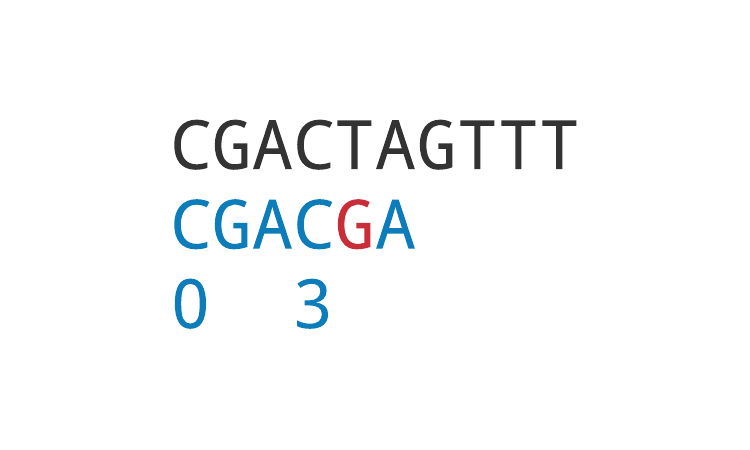
\includegraphics[scale=0.2]{c1/logos/1H.png} 
\end{center}
\hline\vspace{5}

\subsection*{Formatting}
\textbf{Input:} DNA strings \emph{Pattern} and \emph{Text} along with an integer $d$.\\
\noindent \textbf{Output:} A space-separated list of integers containing all starting positions where \emph{Pattern} appears as a substring of \emph{Text} with at most $d$ mismatches.

\subsection*{Constraints}
\begin{itemize}
    \item The length of \emph{Pattern} will be between $1$ and $10^2$.
    \item The length of \emph{Text} will be between $1$ and $10^5$.
    \item The integer $d$ will be between $1$ and $10^1$.
    \item \emph{Pattern} and \emph{Text} will be DNA strings.
\end{itemize}
\pagebreak

\subsection*{\href{https://github.com/rjeveloff/BA_problemregister/tree/main/test_cases/chapter_1/1H}{Test Cases \gitlogo}}
\stepcounter{subsubsection}\subsubsection*{Case \arabic{subsubsection}}
\hline \vspace{5}
\textbf{Description:} The sample dataset is not actually run on your code.\\ \\
\noindent \textbf{Input:}\\
\code{ATTCTGGA\\CGCCCGAATCCAGAACGCATTCCCATATTTCGGGACCACTGGCCTCCACGGTACGGACGTCAATCAAAT\\3}\\ \\
\noindent \textbf{Output:}\\
\code{6 7 26 27}

\stepcounter{subsubsection}\subsubsection*{Case \arabic{subsubsection}}
\hline \vspace{5}
\textbf{Description:} This dataset checks if you are only counting instances where the number of mismatches is
exactly equal to $d$ (i.e. ignoring instances where mismatch < $d$).\\ \\
\noindent \textbf{Input:}\\
\code{AAA\\TTTTTTAAATTTTAAATTTTTT\\2}\\ \\
\noindent \textbf{Output:}\\
\code{4 5 6 7 8 11 12 13 14 15}

\stepcounter{subsubsection}\subsubsection*{Case \arabic{subsubsection}}
\hline \vspace{5}
\textbf{Description:} This dataset checks if your code has an off-by-one error at the beginning of \emph{Text} (i.e. your code is not checking the the left-most substring of \emph{Text}).\\ \\
\noindent \textbf{Input:}\\
\code{GAGCGCTGG\\GAGCGCTGGGTTAACTCGCTACTTCCCGACGAGCGCTGTGGCGCAAATTGGCGATGAAACTGCAGAGAGAACTG\dots\\
\dots GTCATCCAACTGAATTCTCCCCGCTATCGCATTTTGATGCGCGCCGCGTCGATT\\2}\\ \\
\noindent \textbf{Output:}\\
\code{0 30 66}
\pagebreak

\stepcounter{subsubsection}\subsubsection*{Case \arabic{subsubsection}}
\hline \vspace{5}
\textbf{Description:} This dataset checks if your code has an off-by-one error at the end of \emph{Text} (i.e. your code is not checking the the right-most substring of \emph{Text}).\\ \\
\noindent \textbf{Input:}\\
\code{AATCCTTTCA\\CCAAATCCCCTCATGGCATGCATTCCCGCAGTATTTAATCCTTTCATTCTGCATATAAGTAGTGAAGGT\dots\\
\dots ATAGAAACCCGTTCAAGCCCGCAGCGGTAAAACCGAGAACCATGATGAATGCACGGCGATTGCGCC\dots\\
\dots ATAATCCAAACA\\3}\\ \\
\noindent \textbf{Output:}\\
\code{3 36 74 137}

\stepcounter{subsubsection}\subsubsection*{Case \arabic{subsubsection}}
\hline \vspace{5}
\textbf{Description:} This dataset checks if your code is correctly accounting for overlapping instances of \emph{Pattern} in \emph{Text}.\\ \\
\noindent \textbf{Input:}\\
\code{CCGTCATCC\\CCGTCATCCGTCATCCTCGCCACGTTGGCATGCATTCCGTCATCCCGTCAGGCATACTTCTGCATATAA\dots\\
\dots GTACAAACATCCGTCATGTCAAAGGGAGCCCGCAGCGGTAAAACCGAGAACCATGATGAATGCACG\dots\\
\dots GCGATTGC\\3}\\ \\
\noindent \textbf{Output:}\\
\code{0 7 36 44 48 72 79 112}

\stepcounter{subsubsection}\subsubsection*{Case \arabic{subsubsection}}
\hline \vspace{5}
\textbf{Description:} This dataset checks if you are only counting instances of \emph{Pattern} with less than $d$ mismatches (as opposed to instances of \emph{Pattern} with less than or equal to $d$ mismatches).\\ \\
\noindent \textbf{Input:}\\
\code{TTT\\AAAAAA\\3}\\ \\
\noindent \textbf{Output:}\\
\code{0 1 2 3}
\pagebreak

\stepcounter{subsubsection}\subsubsection*{Case \arabic{subsubsection}}
\hline \vspace{5}
\textbf{Description:} This dataset checks if your code works with input where $d=0$ (i.e. only perfect matches are allowed).\\ \\
\noindent \textbf{Input:}\\
\code{CCA\\CCACCT\\0}\\ \\
\noindent \textbf{Output:}\\
\code{0}

\stepcounter{subsubsection}\subsubsection*{Case \arabic{subsubsection}}
\hline \vspace{5}
\textbf{Description:} A larger dataset of the same size as that provided by the randomized autograder. Check input/output folders for this dataset.\\ \\
\pagebreak
%                                                                                                                           PROBLEM BREAK
\subsection{Find the Most Frequent Words with Mismatches in a String}
\hline\vspace{5}
\noindent \textbf{Frequent Words with Mismatches Problem}\\
\emph{Find the most frequent $k$-mers with mismatches in a string}.\\ \\
\textbf{Input:} A DNA string \emph{Text} as well as integers $k$ and $d$.\\
\textbf{Output:} All most frequent $k$-mers with up to $d$ mismatches in \emph{Text}.
\begin{center}
    
\includegraphics[scale=0.2]{c1/logos/1I.png} 
\end{center}
\hline\vspace{5}

\subsection*{Formatting}
\textbf{Input:} A DNA string \emph{Text} as well as integers $k$ and $d$.\\
\noindent \textbf{Output:} A space-separated list of strings representing all most frequent $k$-mers with up to $d$ mismatches in \emph{Text}.

\subsection*{Constraints}
\begin{itemize}
    \item The length of \emph{Text} will be between $1$ and $10^3$.
    \item The integer $k$ will be between $1$ and $10^1$.
    \item The integer $d$ will be between $1$ and $10^1$.
    \item \emph{Text} will be a DNA string.
\end{itemize}
\pagebreak

\subsection*{\href{https://github.com/rjeveloff/BA_problemregister/tree/main/test_cases/chapter_1/1I}{Test Cases \gitlogo}}
\stepcounter{subsubsection}\subsubsection*{Case \arabic{subsubsection}}
\hline \vspace{5}
\textbf{Description:} The sample dataset is not actually run on your code.\\ \\
\noindent \textbf{Input:}\\
\code{ACGTTGCATGTCGCATGATGCATGAGAGCT\\4 1}\\ \\
\noindent \textbf{Output:}\\
\code{ATGC ATGT GATG}

\stepcounter{subsubsection}\subsubsection*{Case \arabic{subsubsection}}
\hline \vspace{5}
\textbf{Description:} \emph{Text} contains partial and complete matches for the most frequent word.\\ \\
\noindent \textbf{Input:}\\
\code{AGGT\\2 1}\\ \\
\noindent \textbf{Output:}\\
\code{GG}

\stepcounter{subsubsection}\subsubsection*{Case \arabic{subsubsection}}
\hline \vspace{5}
\textbf{Description:} $d = 0$.\\ \\
\noindent \textbf{Input:}\\
\code{AGGGT\\2 0}\\ \\
\noindent \textbf{Output:}\\
\code{GG}

\stepcounter{subsubsection}\subsubsection*{Case \arabic{subsubsection}}
\hline \vspace{5}
\textbf{Description:} \emph{Text} has multiple most frequent words.\\ \\
\noindent \textbf{Input:}\\
\code{AGGCGG\\3 0}\\ \\
\noindent \textbf{Output:}\\
\code{AGG GGC GCG CGG}
\pagebreak

\stepcounter{subsubsection}\subsubsection*{Case \arabic{subsubsection}}
\hline \vspace{5}
\textbf{Description:} A larger dataset of the same size as that provided by the randomized autograder. Check input/output folders for this dataset.\\ \\
\pagebreak
%                                                                                                                           PROBLEM BREAK
\subsection{Find Frequent Words with Mismatches and Reverse Complements}
\hline\vspace{5}
\noindent \textbf{Frequent Words with Mismatches and Reverse Complements Problem}\\
\emph{Find the most frequent $k$-mers (with mismatches and reverse complements) in a DNA string}.\\ \\
\textbf{Input:} A DNA string \emph{Text} as well as integers $k$ and $d$.\\
\textbf{Output:} All $k$-mers \emph{Pattern} maximizing the sum \sc{Count}$_d$(\emph{Text}, \emph{Pattern})$+$\sc{Count}$_d$(\emph{Text}, $\overline{Pattern}$) over all possible $k$-mers.
\begin{center}
    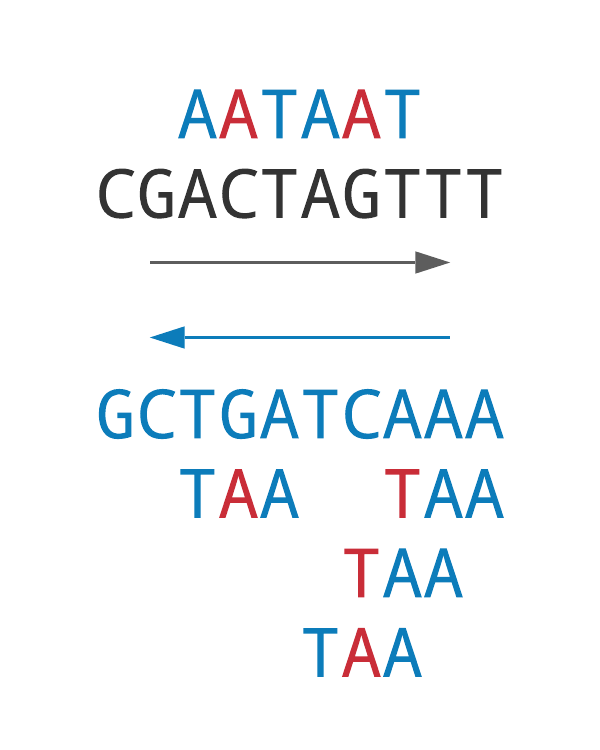
\includegraphics[scale=0.2]{c1/logos/1J.png} 
\end{center}
\hline\vspace{5}

\subsection*{Formatting}
\textbf{Input:} A DNA string \emph{Text} as well as integers $k$ and $d$.\\
\noindent \textbf{Output:} A space-separated list of strings representing all $k$-mers \emph{Pattern} maximizing the sum \sc{Count}$_d$(\emph{Text}, \emph{Pattern})$+$\sc{Count}$_d$(\emph{Text}, $\overline{Pattern}$) over all possible $k$-mers.

\subsection*{Constraints}
\begin{itemize}
    \item The length of \emph{Text} will be between $1$ and $10^3$.
    \item The integer $k$ will be between $1$ and $10^1$.
    \item The integer $d$ will be between $1$ and $10^1$.
    \item \emph{Text} will be a DNA string.
\end{itemize}
\pagebreak

\subsection*{\href{https://github.com/rjeveloff/BA_problemregister/tree/main/test_cases/chapter_1/1J}{Test Cases \gitlogo}}
\stepcounter{subsubsection}\subsubsection*{Case \arabic{subsubsection}}
\hline \vspace{5}
\textbf{Description:} The sample dataset is not actually run on your code.\\ \\
\noindent \textbf{Input:}\\
\code{ACGTTGCATGTCGCATGATGCATGAGAGCT\\4 1}\\ \\
\noindent \textbf{Output:}\\
\code{ACAT ATGT}

\stepcounter{subsubsection}\subsubsection*{Case \arabic{subsubsection}}
\hline \vspace{5}
\textbf{Description:} \emph{Text} contains partial and completes matches for the most frequent word.\\ \\
\noindent \textbf{Input:}\\
\code{AAAAAAAAAA\\2 1}\\ \\
\noindent \textbf{Output:}\\
\code{AT TA}

\stepcounter{subsubsection}\subsubsection*{Case \arabic{subsubsection}}
\hline \vspace{5}
\textbf{Description:} This dataset makes sure that your code is not accidentally swapping $k$ and $d$.\\ \\
\noindent \textbf{Input:}\\
\code{AGTCAGTC\\4 2}\\ \\
\noindent \textbf{Output:}\\
\code{AATT GGCC}

\stepcounter{subsubsection}\subsubsection*{Case \arabic{subsubsection}}
\hline \vspace{5}
\textbf{Description:} This dataset makes sure you are finding $k$-mers in both \emph{Text} and the reverse complement of \emph{Text}.\\ \\
\noindent \textbf{Input:}\\
\code{AATTAATTGGTAGGTAGGTA\\4 0}\\ \\
\noindent \textbf{Output:}\\
\code{AATT}
\pagebreak

\stepcounter{subsubsection}\subsubsection*{Case \arabic{subsubsection}}
\hline \vspace{5}
\textbf{Description:} This dataset first checks that $k$-mers with exactly $d$ mismatches are being found. Then, it
checks that $k$-mers with less than $d$ mismatches are being allowed (i.e. you are not only allowing $k$-mers with exactly $d$ mismatches). Next, it checks that you are not returning too few $k$-mers. Last, it checks that you are not returning too many $k$-mers.\\ \\
\noindent \textbf{Input:}\\
\code{ATA\\3 1}\\ \\
\noindent \textbf{Output:}\\
\code{AAA AAT ACA AGA ATA ATC ATG ATT CAT CTA GAT GTA TAA TAC TAG TAT
TCT TGT TTA TTT}

\stepcounter{subsubsection}\subsubsection*{Case \arabic{subsubsection}}
\hline \vspace{5}
\textbf{Description:} This dataset checks that your code is looking at \emph{both} \emph{Text} and its reverse complement (i.e. not just looking at \emph{Text}, and not just looking at the reverse complement of \emph{Text}, but looking at both).\\ \\
\noindent \textbf{Input:}\\
\code{AAT\\3 0}\\ \\
\noindent \textbf{Output:}\\
\code{AAT ATT}

\stepcounter{subsubsection}\subsubsection*{Case \arabic{subsubsection}}
\hline \vspace{5}
\textbf{Description:} This dataset checks that your code correctly delimiting your output (i.e. using spaces) and
verifies that your $k$-mers are actually of length $k$.\\ \\
\noindent \textbf{Input:}\\
\code{TAGCG\\2 1}\\ \\
\noindent \textbf{Output:}\\
\code{CA CC GG TG}

\stepcounter{subsubsection}\subsubsection*{Case \arabic{subsubsection}}
\hline \vspace{5}
\textbf{Description:} A larger dataset of the same size as that provided by the randomized autograder. Check input/output folders for this dataset.\\ \\
\pagebreak
%                                                                                                                           PROBLEM BREAK
\subsection{Generate the Frequency Array of a String}
\hline\vspace{5}
\noindent \textbf{Frequency Array Problem}\\
\emph{Generate the frequency array of a DNA string}.\\ \\
\textbf{Input:} A DNA string \emph{Text} and an integer $k$.\\
\textbf{Output:} The frequency array of $k$-mers in \emph{Text}.
\begin{center}
    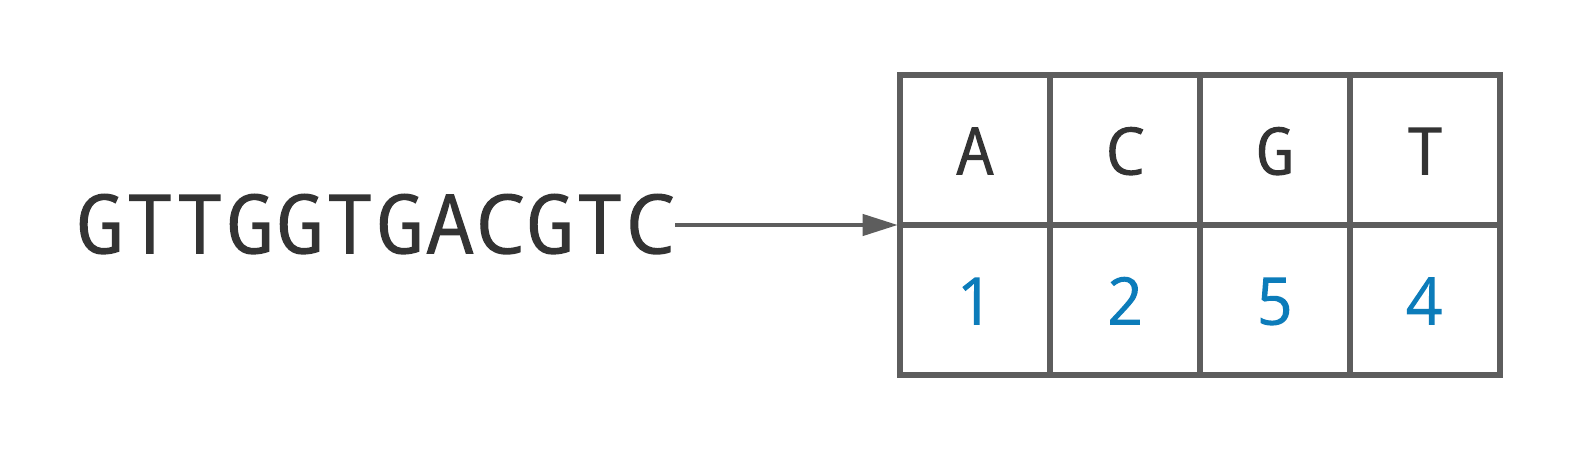
\includegraphics[scale=0.2]{c1/logos/1K.png} 
\end{center}
\hline\vspace{5}

\subsection*{Formatting}
\textbf{Input:} A DNA string \emph{Text} and an integer $k$.\\
\noindent \textbf{Output:} A space-separated list of integers representing the frequency array of $k$-mers in \emph{Text}).

\subsection*{Constraints}
\begin{itemize}
    \item The length of \emph{Text} will be between $1$ and $10^3$.
    \item The integer $k$ will be between $1$ and $10^1$.
    \item \emph{Text} will be a DNA string.
\end{itemize}
\pagebreak

\subsection*{\href{https://github.com/rjeveloff/BA_problemregister/tree/main/test_cases/chapter_1/1K}{Test Cases \gitlogo}}
\stepcounter{subsubsection}\subsubsection*{Case \arabic{subsubsection}}
\hline \vspace{5}
\textbf{Description:} The sample dataset is not actually run on your code.\\ \\
\noindent \textbf{Input:}\\
\code{ACGCGGCTCTGAAA\\2}\\ \\
\noindent \textbf{Output:}\\
\code{2 1 0 0 0 0 2 2 1 2 1 0 0 1 1 0}

\stepcounter{subsubsection}\subsubsection*{Case \arabic{subsubsection}}
\hline \vspace{5}
\textbf{Description:} This dataset checks if you have an off-by-one error at the end of \emph{Text} (i.e. you are not
counting the last $k$-mer in \emph{Text}). There are three instances of \code{AA} (\codebold{AA}\code{AAC}, \code{A}\codebold{AA}\code{AC}, and \code{AA}\codebold{AA}\code{C}), but there is one instance of \code{AC} at the end (\code{AAA}\codebold{AC}).\\ \\
\noindent \textbf{Input:}\\
\code{AAAAC\\2}\\ \\
\noindent \textbf{Output:}\\
\code{3 1 0 0 0 0 0 0 0 0 0 0 0 0 0 0}

\stepcounter{subsubsection}\subsubsection*{Case \arabic{subsubsection}}
\hline \vspace{5}
\textbf{Description:} This dataset checks if you have an off-by-one error at the beginning of \emph{Text} (i.e. you are not counting the first $k$-mer in \emph{Text}). There are two instances of \code{AA} (\code{TT}\codebold{AA}\code{A} and \code{TTA}\codebold{AA}), but there is one instance of \code{TA} (\code{T}\codebold{TA}\code{AA}) and one instance of \code{TT} (\codebold{TT}\code{AAA}).\\ \\
\noindent \textbf{Input:}\\
\code{TTAAA\\2}\\ \\
\noindent \textbf{Output:}\\
\code{2 0 0 0 0 0 0 0 0 0 0 0 1 0 0 1}
\pagebreak

\stepcounter{subsubsection}\subsubsection*{Case \arabic{subsubsection}}
\hline \vspace{5}
\textbf{Description:} This dataset checks if your code actually increments each count, or if your code instead
just sets the count equal to one each time. In other words, this dataset checks if your code is doing something like array[$k$-mer]$=1$ instead of array[$k$-mer]$+=1$.\\ \\
\noindent \textbf{Input:}\\
\code{AAA\\2}\\ \\
\noindent \textbf{Output:}\\
\code{2 0 0 0 0 0 0 0 0 0 0 0 0 0 0 0}

\stepcounter{subsubsection}\subsubsection*{Case \arabic{subsubsection}}
\hline \vspace{5}
\textbf{Description:} A larger dataset of the same size as that provided by the randomized autograder. Check input/output folders for this dataset.\\ \\
\pagebreak
%                                                                                                                           PROBLEM BREAK
\subsection{Implement PatternToNumber}
\hline\vspace{5}
\noindent \textbf{PatternToNumber Problem}\\
\emph{Convert a DNA string to a number}.\\ \\
\textbf{Input:} A DNA string \emph{Pattern}.\\
\textbf{Output:} \sc{PatternToNumber}(\emph{Pattern}).
\begin{center}
    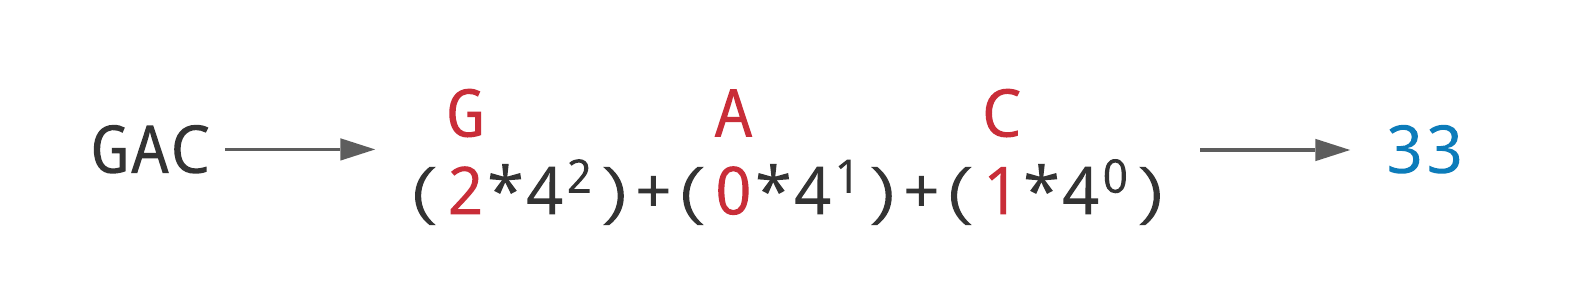
\includegraphics[scale=0.2]{c1/logos/1L.png} 
\end{center}
\hline\vspace{5}

\subsection*{Formatting}
\textbf{Input:} A DNA string \emph{Pattern}.\\
\noindent \textbf{Output:} An integer representing the output of \sc{PatternToNumber}(\emph{Pattern}).

\subsection*{Constraints}
\begin{itemize}
    \item The length of \emph{Pattern} will be between $1$ and $10^2$.
    \item \emph{Pattern} will be a DNA string.
\end{itemize}
\pagebreak
\subsection*{\href{https://github.com/rjeveloff/BA_problemregister/tree/main/test_cases/chapter_1/1L}{Test Cases \gitlogo}}
\stepcounter{subsubsection}\subsubsection*{Case \arabic{subsubsection}}
\hline \vspace{5}
\textbf{Description:} The sample dataset is not actually run on your code.\\ \\
\noindent\textbf{Input:}\\
\code{
AGT
}\\ \\
\noindent\textbf{Output:}\\
\code{
11
}

\stepcounter{subsubsection}\subsubsection*{Case \arabic{subsubsection}}
\hline \vspace{5}
\textbf{Description:} \emph{Pattern} is made up of only one character.\\ \\
\noindent \textbf{Input:}\\
\code{CCC}\\ \\
\noindent \textbf{Output:}\\
\code{21}

\stepcounter{subsubsection}\subsubsection*{Case \arabic{subsubsection}}
\hline \vspace{5}
\textbf{Description:} \emph{Pattern} is long, but is 'A'-dense.\\ \\
\noindent \textbf{Input:}\\
\code{AAAAAAAAAAG}\\ \\
\noindent \textbf{Output:}\\
\code{2}

\stepcounter{subsubsection}\subsubsection*{Case \arabic{subsubsection}}
\hline \vspace{5}
\textbf{Description:} \emph{Pattern} has a length of 1.\\ \\
\noindent \textbf{Input:}\\
\code{T}\\ \\
\noindent \textbf{Output:}\\
\code{3}

\stepcounter{subsubsection}\subsubsection*{Case \arabic{subsubsection}}
\hline \vspace{5}
\textbf{Description:} A larger dataset of the same size as that provided by the randomized autograder. Check input/output folders for this dataset.\\ \\
\pagebreak
%                                                                                                                           PROBLEM BREAK
\subsection{Implement NumberToPattern}
\hline\vspace{5}
\noindent \textbf{NumberToPattern Problem}\\
\emph{Convert a number to its corresponding DNA string}.\\ \\
\textbf{Input:} Integers \emph{index} and $k$.\\
\textbf{Output:} \sc{NumberToPattern}(\emph{index}, $k$).
\begin{center}
    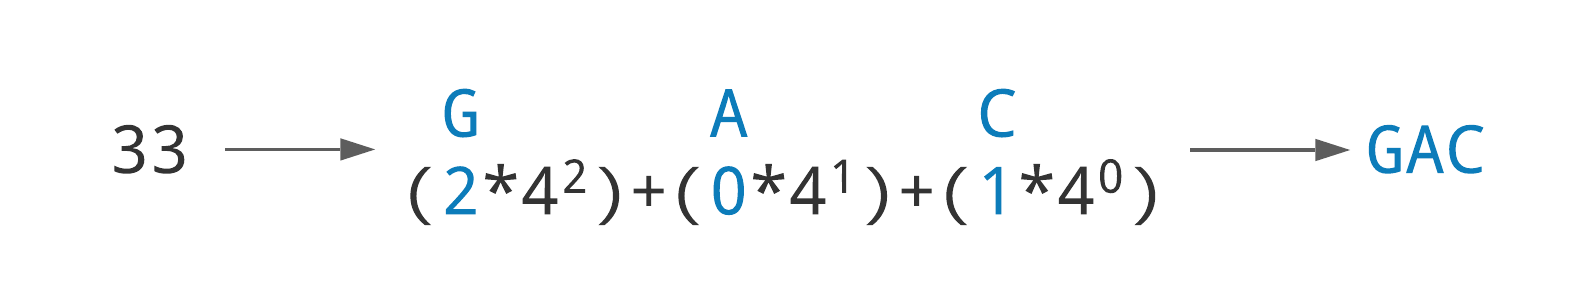
\includegraphics[scale=0.2]{c1/logos/1M.png} 
\end{center}
\hline\vspace{5}

\subsection*{Formatting}
\textbf{Input:} Space-separated integers \emph{index} and $k$.\\
\noindent \textbf{Output:} A string representing the output of \emph{NumberToPattern}(\emph{index}, $k$).

\subsection*{Constraints}
\begin{itemize}
    \item The integer \emph{index} will be between $1$ and $10^4$.
    \item The integer $k$ will be between $1$ and $10^1$.
\end{itemize}
\pagebreak

\subsection*{\href{https://github.com/rjeveloff/BA_problemregister/tree/main/test_cases/chapter_1/1M}{Test Cases \gitlogo}}
\stepcounter{subsubsection}\subsubsection*{Case \arabic{subsubsection}}
\hline \vspace{5}
\textbf{Description:} The sample dataset is not actually run on your code.\\ \\
\noindent \textbf{Input:}\\
\code{45 4}\\ \\
\noindent \textbf{Output:}\\
\code{AGTC}

\stepcounter{subsubsection}\subsubsection*{Case \arabic{subsubsection}}
\hline \vspace{5}
\textbf{Description:} \emph{k} is small.\\ \\
\noindent \textbf{Input:}\\
\code{1 8}\\ \\
\noindent \textbf{Output:}\\
\code{G}

\stepcounter{subsubsection}\subsubsection*{Case \arabic{subsubsection}}
\hline \vspace{5}
\textbf{Description:} \emph{k} codes for an empty string\\ \\
\noindent \textbf{Input:}\\
\code{0 0}\\ \\
\noindent \textbf{Output:}
\\

\stepcounter{subsubsection}\subsubsection*{Case \arabic{subsubsection}}
\hline \vspace{5}
\textbf{Description:} \emph{k} is large.\\ \\
\noindent\textbf{Input:} Space-separated integers $k$ and $d$ followed by a space-separated list of paired $k$-mer strings \emph{PairedReads} where individual $k$-mers within the pair are separated by a "|" character.\\
\noindent \textbf{Input:}\\
\code{60 4}\\ \\
\noindent \textbf{Output:}\\
\code{ATTA}
\pagebreak

\stepcounter{subsubsection}\subsubsection*{Case \arabic{subsubsection}}
\hline \vspace{5}
\textbf{Description:} A larger dataset of the same size as that provided by the randomized autograder. Check input/output folders for this dataset.\\ \\
\pagebreak
%                                                                                                                           PROBLEM BREAK
\subsection{Generate the $d$-Neighborhood of a String}
\hline\vspace{5}
\noindent \textbf{$d$-Neighborhood Problem}\\
\emph{Find all the neighbors of a pattern}.\\ \\
\textbf{Input:} A DNA string \emph{Pattern} and an integer $d$.\\
\textbf{Output:} The collection of strings \sc{Neighbors}(\emph{Pattern}, $d$).
\begin{center}
    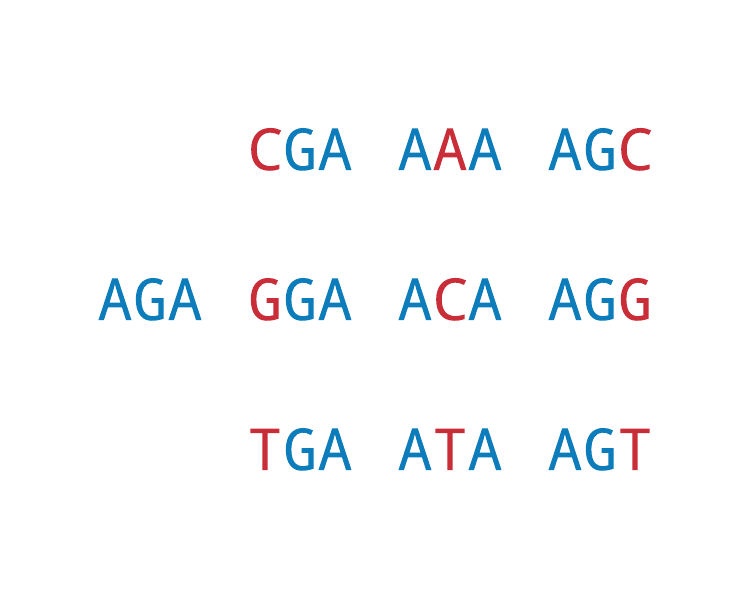
\includegraphics[scale=0.24]{c1/logos/1N.png} 
\end{center}
\hline\vspace{5}

\subsection*{Formatting}
\textbf{Input:} A DNA string \emph{Pattern} and an integer $d$.\\
\noindent \textbf{Output:} A space-separated list of strings containing all \emph{Neighbors}(\emph{Pattern}, $d$).

\subsection*{Constraints}
\begin{itemize}
    \item The length of \emph{Pattern} will be between $1$ and $10^1$.
    \item The integer $d$ will be between $1$ and $10^1$.
    \item \emph{Pattern} will be a DNA string.
\end{itemize}
\pagebreak

\subsection*{\href{https://github.com/rjeveloff/BA_problemregister/tree/main/test_cases/chapter_1/1N}{Test Cases \gitlogo}}
\stepcounter{subsubsection}\subsubsection*{Case \arabic{subsubsection}}
\hline \vspace{5}
\textbf{Description:} The sample dataset is not actually run on your code.\\ \\
\noindent \textbf{Input:}\\
\code{
ACG \\
1
}\\ \\
\noindent \textbf{Output:}\\
\code{
AAG ACA ACC ACG ACT AGG ATG CCG GCG TCG
}

\stepcounter{subsubsection}\subsubsection*{Case \arabic{subsubsection}}
\hline \vspace{5}
\textbf{Description:} $d = 0$.\\ \\
\noindent \textbf{Input:}\\
\code{AGA\\ 0}\\ \\
\noindent \textbf{Output:}\\
\code{AGA}

\stepcounter{subsubsection}\subsubsection*{Case \arabic{subsubsection}}
\hline \vspace{5}
\textbf{Description:} \emph{Pattern} is made up of one character.\\ \\
\noindent \textbf{Input:}\\
\code{AAA\\ 1}\\ \\
\noindent \textbf{Output:}\\
\code{AAA AAC AAG AAT ACA AGA ATA CAA GAA TAA}

\stepcounter{subsubsection}\subsubsection*{Case \arabic{subsubsection}}
\hline \vspace{5}
\textbf{Description:} \emph{Pattern} has a length of 1.\\ \\
\noindent \textbf{Input:}\\
\code{A\\ 1}\\ \\
\noindent \textbf{Output:}\\
\code{A C G T}
\pagebreak

\stepcounter{subsubsection}\subsubsection*{Case \arabic{subsubsection}}
\hline \vspace{5}
\textbf{Description:} A larger dataset of the same size as that provided by the randomized autograder. Check input/output folders for this dataset.\\ \\
\pagebreak

\subsection{Implement ApproximatePatternCount}
\hline\vspace{5}
\noindent \textbf{Approximate Pattern Count Problem}\\
\emph{Count all approximate occurrences of a pattern in a string}.\\ \\
\textbf{Input:} Strings \emph{Pattern} and \emph{Text} as well as an integer $d$.\\
\textbf{Output:} \sc{Count}$_d$(\emph{Text}, \emph{Pattern}).
\begin{center}
    
\includegraphics[scale=0.24]{c1/logos/1O.png} 
\end{center}
\hline\vspace{5}

\subsection*{Formatting}
\textbf{Input:} A DNA string \emph{Pattern} followed by a DNA string \emph{Text}, followed by an integer $d$.\\
\noindent \textbf{Output:} A single integer \sc{Count}$_d$(\emph{Text}, \emph{Pattern}).

\subsection*{Constraints}
\begin{itemize}
    \item The length of \emph{Pattern} will be between $1$ and $10^1$.
    \item The length of \emph{Text} will be between $1$ and $10^3$
    \item The integer $d$ will be between $1$ and $10^1$.
    \item Both \emph{Pattern} \emph{Text} and will be DNA strings.
\end{itemize}
\pagebreak

\subsection*{\href{https://github.com/rjeveloff/BA_problemregister/tree/main/test_cases/chapter_1/1O}{Test Cases \gitlogo}}
\stepcounter{subsubsection}\subsubsection*{Case \arabic{subsubsection}}
\hline \vspace{5}
\textbf{Description:} The sample dataset is not actually run on your code.\\ \\
\noindent \textbf{Input:}\\
\code{GAGG\\TTTAGAGCCTTCAGAGG\\2}\\ \\
\noindent \textbf{Output:}\\
\code{4}

\stepcounter{subsubsection}\subsubsection*{Case \arabic{subsubsection}}
\hline \vspace{5}
\textbf{Description:} A larger dataset of the same size as that provided by the randomized autograder. Check input/output folders for this dataset.\\ \\
\pagebreak
%                                                                                                                           PROBLEM BREAK
\section{Which DNA Patterns Play the Role of Molecular Clocks?\\ \normalfont\emph{Randomized Algorithms}}
\begin{center}
    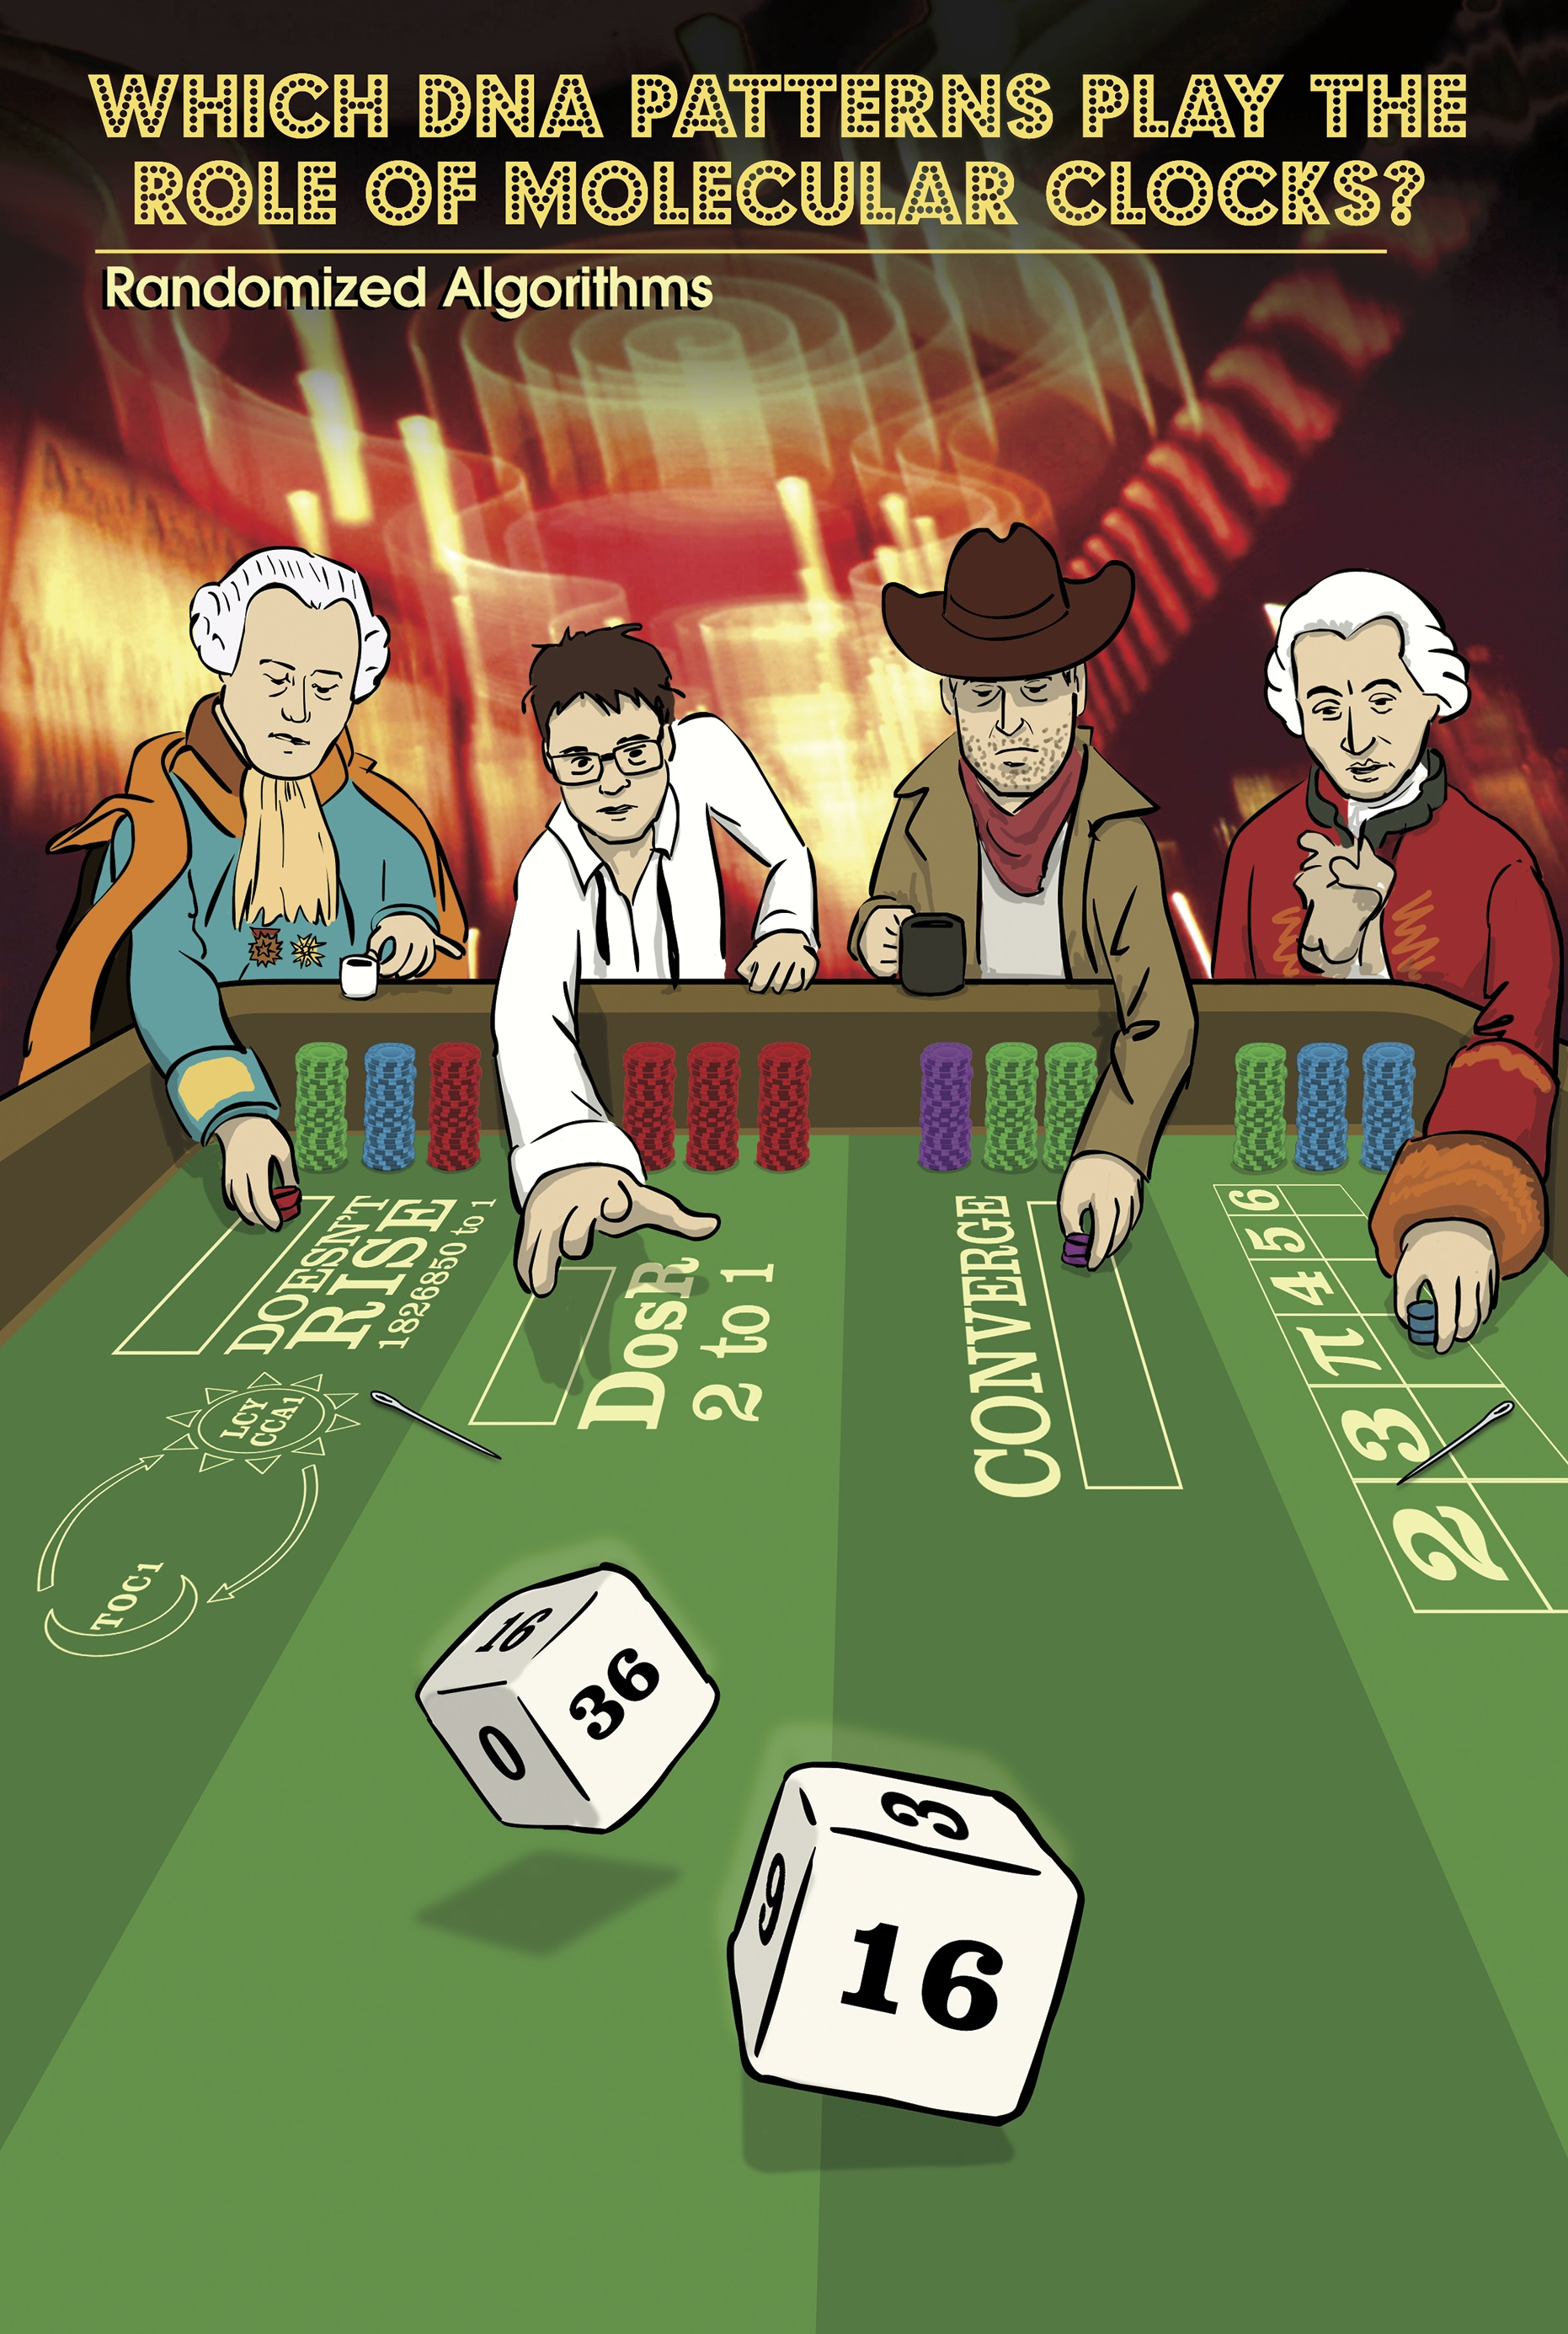
\includegraphics[scale=0.72]{c2/c2.jpg}
\end{center}
\pagebreak

\subsection{Implement MotifEnumeration}
\hline\vspace{5}
\noindent\textbf{Implanted Motif Problem}\\
\emph{Find all ($k$, $d$)-motifs in a collection of strings}.\\ \\
\textbf{Input:} A collection of strings \emph{Dna}, and integers $k$ and $d$.\\
\textbf{Output:} All ($k$, $d$)-motifs in \emph{Dna}.
\begin{center}
    
\includegraphics[scale=0.24]{c2/logos/2A.png} 
\end{center}
\hline\vspace{5}

\subsection*{Formatting}
\textbf{Input:} Space-separated integers $k$ and $d$, followed by a space-separated collection of strings \emph{Dna}.\\
\noindent\textbf{Output:} A space-separated list of strings representing all ($k$, $d$)-motifs in \emph{Dna}.

\subsection*{Constraints}
\begin{itemize}
    \item The integer $k$ will be between $1$ and $10^1$.
    \item The integer $d$ will be between $1$ and $10^1$.
    \item The number of strings in \emph{Dna} will be between $1$ and $10^2$.
    \item Each string in \emph{Dna} will have a length between $1$ and $10^2$.
    \item All strings in \emph{Dna} will be DNA strings.
\end{itemize}
\pagebreak

\subsection*{\href{https://github.com/rjeveloff/BA_problemregister/tree/main/test_cases/chapter_2/2A}{Test Cases \gitlogo}}
\stepcounter{subsubsection}\subsubsection*{Case \arabic{subsubsection}}
\hline \vspace{5}
\textbf{Description:} The sample dataset is not actually run on your code.\\ \\
\noindent \textbf{Input:}\\
\code{3 1\\ATTTGGC TGCCTTA CGGTATC GAAAATT}\\ \\
\noindent \textbf{Output:}\\
\code{ATA ATT GTT TTT}

\stepcounter{subsubsection}\subsubsection*{Case \arabic{subsubsection}}
\hline \vspace{5}
\textbf{Description:} This dataset checks for off-by-one errors, both at the beginning and at the end. The $3$-mers \code{ACG} and \code{CGT} both appear perfectly in all $3$ strings in \emph{Dna}. Thus, if your output doesn’t contain \code{ACG}, you are most likely not counting the first $k$-mer of every string. Similarly, if your output doesn’t contain \code{CGT}, you are most likely not counting the last $k$-mer of every string.  \\ \\
\noindent \textbf{Input:}\\
\code{3 0\\ACGT ACGT ACGT}\\ \\
\noindent \textbf{Output:}\\
\code{ACG CGT}

\stepcounter{subsubsection}\subsubsection*{Case \arabic{subsubsection}}
\hline \vspace{5}
\textbf{Description:} This dataset checks if your code work correctly when $d>0$. If your code only counts motifs with $d=0$ (and not $d>0$), your code will only find a single motif (\code{AAA}, which is the only $3$-mer that occurs perfectly in all of the strings of \emph{Dna}). A correct solution would, in addition to \code{AAA}, find all $3$-mers that differ from \code{AAA} by exactly $1$ base.\\ \\
\noindent \textbf{Input:}\\
\code{3 1\\AAAAA AAAAA AAAAA}\\ \\
\noindent \textbf{Output:}\\
\code{AAA AAC AAG AAT ACA AGA ATA CAA GAA TAA}
\pagebreak

\stepcounter{subsubsection}\subsubsection*{Case \arabic{subsubsection}}
\hline \vspace{5}
\textbf{Description:} This dataset checks if your code counts motifs where the number of mismatches is equal to $d$ in addition to motifs where the number of mismatches is less than $d$. For example, in this dataset, a correct solution would find \emph{all} $3$-mers (because we are allowing for $3$ mismatches). However, an incorrect solution that counts mismatches less than $d$ but not mismatches equal to $d$ would only find the $k$-mers that differ from \code{AAA} by $1$ or $2$ bases, not the ones that differ from \code{AAA} by $3$ bases.\\ \\
\noindent \textbf{Input:}\\
\code{3 3\\AAAAA AAAAA AAAAA}\\ \\
\noindent \textbf{Output:}\\
\code{AAA AAC AAG AAT ACA ACC ACG ACT AGA AGC AGG AGT ATA ATC ATG ATT CAA CAC CAG CAT CCA CCC CCG CCT CGA CGC CGG CGT CTA CTC CTG CTT GAA GAC GAG GAT GCA GCC GCG GCT GGA GGC GGG GGT GTA GTC GTG GTT TAA TAC TAG TAT TCA TCC TCG TCT TGA TGC TGG TGT TTA TTC TTG TTT}

\stepcounter{subsubsection}\subsubsection*{Case \arabic{subsubsection}}
\hline \vspace{5}
\textbf{Description:} This test dataset checks if your code is checking the last sequence in \emph{Dna}. If your code only checks the first two sequences in the dataset, the $3$-mer \code{AAA} exists perfectly in both and will thus be output. If your code checks the last sequence of \emph{Dna} (\code{AACAA}), however, it will find that \code{AAA} does not appear. Thus, \code{AAA} is not a motif in \emph{Dna}, and no sequences should be output.\\ \\
\noindent \textbf{Input:}\\
\code{3 0\\AAAAA AAAAA AACAA}\\ \\
\noindent \textbf{Output:}\\
\code{}

\stepcounter{subsubsection}\subsubsection*{Case \arabic{subsubsection}}
\hline \vspace{5}
\textbf{Description:} This test dataset checks if your code is checking the first sequence in \emph{Dna}. If your code only checks the last two sequences in the dataset, the $3$-mer \code{AAA} exists perfectly in both and will thus be output. If your code checks the first sequence of \emph{Dna} (\code{AACAA}), however, it will find that \code{AAA} does not appear. Thus, \code{AAA} is not a motif in \emph{Dna}, and no sequences should be output.\\ \\
\noindent \textbf{Input:}\\
\code{3 0\\AACAA AAAAA AAAAA}\\ \\
\noindent \textbf{Output:}\\
\code{}
\pagebreak

\stepcounter{subsubsection}\subsubsection*{Case \arabic{subsubsection}}
\hline \vspace{5}
\textbf{Description:} A larger dataset of the same size as that provided by the randomized autograder. Check input/output folders for this dataset.\\ \\
\pagebreak
%                                                                                                                           PROBLEM BREAK
\subsection{Find a Median String}
\hline\vspace{5}
\noindent\textbf{Median String Problem}\\
\emph{Find a median string}.\\ \\
\textbf{Input:} A collection of strings \emph{Dna} and an integer $k$.\\
\textbf{Output:} A $k$-mer \emph{Pattern} that minimizes \sc{d}(\emph{Pattern}, \emph{Dna}) among all possible choices of $k$-mers.
\begin{center}
    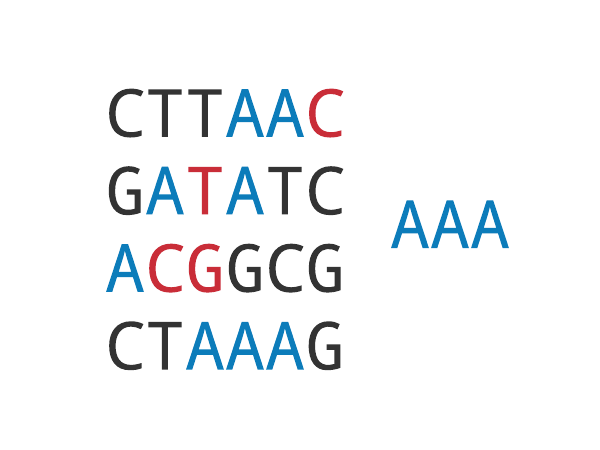
\includegraphics[scale=0.24]{c2/logos/2B.png} 
\end{center}
\hline\vspace{5}

\subsection*{Formatting}
\textbf{Input:} An integer $k$, followed by a newline-separated collection of strings \emph{Dna}.\\
\noindent\textbf{Output:} A string representing a $k$-mer \emph{Pattern} that minimizes \emph{d}(\emph{Pattern}, \emph{Dna}) over all $k$-mers \emph{Pattern} (If multiple answers exist, you may return any one).

\subsection*{Constraints}
\begin{itemize}
    \item The integer $k$ will be between $1$ and $10^1$.
    \item The number of strings in \emph{Dna} will be between $1$ and $10^2$.
    \item The length of each string in \emph{Dna} will be between $1$ and $10^2$.
    \item Each string in \emph{Dna} will be a DNA string.
\end{itemize}
\pagebreak

\subsection*{\href{https://github.com/rjeveloff/BA_problemregister/tree/main/test_cases/chapter_2/2B}{Test Cases \gitlogo}}
\stepcounter{subsubsection}\subsubsection*{Case \arabic{subsubsection}}
\hline \vspace{5}
\textbf{Description:} The sample dataset is not actually run on your code. Notice that there are technically two solutions to the problem (\code{ACG} and \code{GAC} are equally optimal), but the problem specifically states to only return a single output (you can arbitrarily pick any optimal solution).\\ \\
\noindent \textbf{Input:}\\
\code{3\\AAATTGACGCAT GACGACCACGTT CGTCAGCGCCTG GCTGAGCACCGG AGTACGGGACAG}\\ \\
\noindent \textbf{Output:}\\
\code{ACG}

\stepcounter{subsubsection}\subsubsection*{Case \arabic{subsubsection}}
\hline \vspace{5}
\textbf{Description:} This dataset checks that your output is the correct length. Notice that there are technically two solutions to the problem (\code{ACG} and \code{CGT} are equally optimal), but the problem specifically states to only return a single output (you can arbitrarily pick any optimal solution). Also, since $k=3$ in this dataset, we check that your output is exactly of length $k$ (should not be any longer or shorter than this).\\ \\
\noindent \textbf{Input:}\\
\code{3\\ACGT ACGT ACGT}\\ \\
\noindent \textbf{Output:}\\
\code{ACG}

\stepcounter{subsubsection}\subsubsection*{Case \arabic{subsubsection}}
\hline \vspace{5}
\textbf{Description:} This dataset checks if your code considers $k$-mers that do not occur in \emph{Dna}. Notice that the best $3$-mer is \code{AAA}, which does not actually occur in any of the sequences in \emph{Dna}. It is perfectly fine that our optimal median string does not actually occur in any of the sequences in \emph{Dna} (similar to the Frequent Words With Mismatches Problem from chapter one).\\ \\
\noindent \textbf{Input:}\\
\code{3\\ATA ACA AGA AAT AAC}\\ \\
\noindent \textbf{Output:}\\
\code{AAA}
\pagebreak

\stepcounter{subsubsection}\subsubsection*{Case \arabic{subsubsection}}
\hline \vspace{5}
\textbf{Description:} This dataset checks that your output only contains a single $k$-mer. Notice that there are technically two solutions to the problem (\code{AAG} and \code{AAT} are equally optimal), but the problem specifically states to only return a single output (you can arbitrarily pick any optimal solution).\\ \\
\noindent \textbf{Input:}\\
\code{3\\AAG AAT}\\ \\
\noindent \textbf{Output:}\\
\code{AAG}

\stepcounter{subsubsection}\subsubsection*{Case \arabic{subsubsection}}
\hline \vspace{5}
\textbf{Description:} A larger dataset of the same size as that provided by the randomized autograder. Check input/output folders for this dataset.\\ \\
\pagebreak
%                                                                                                                           PROBLEM BREAK
\subsection{Find a Profile-most Probable $k$-mer in a String}
\hline\vspace{5}
\noindent\textbf{Profile-most Probable $k$-mer Problem}\\
\emph{Find a profile-most probable $k$-mer in a string}.\\ \\
\textbf{Input:} A string \emph{Text}, an integer $k$, and a $4\times k$ matrix \emph{Profile}.\\
\textbf{Output:} A \emph{Profile}-most probable $k$-mer in \emph{Text}.
\begin{center}
    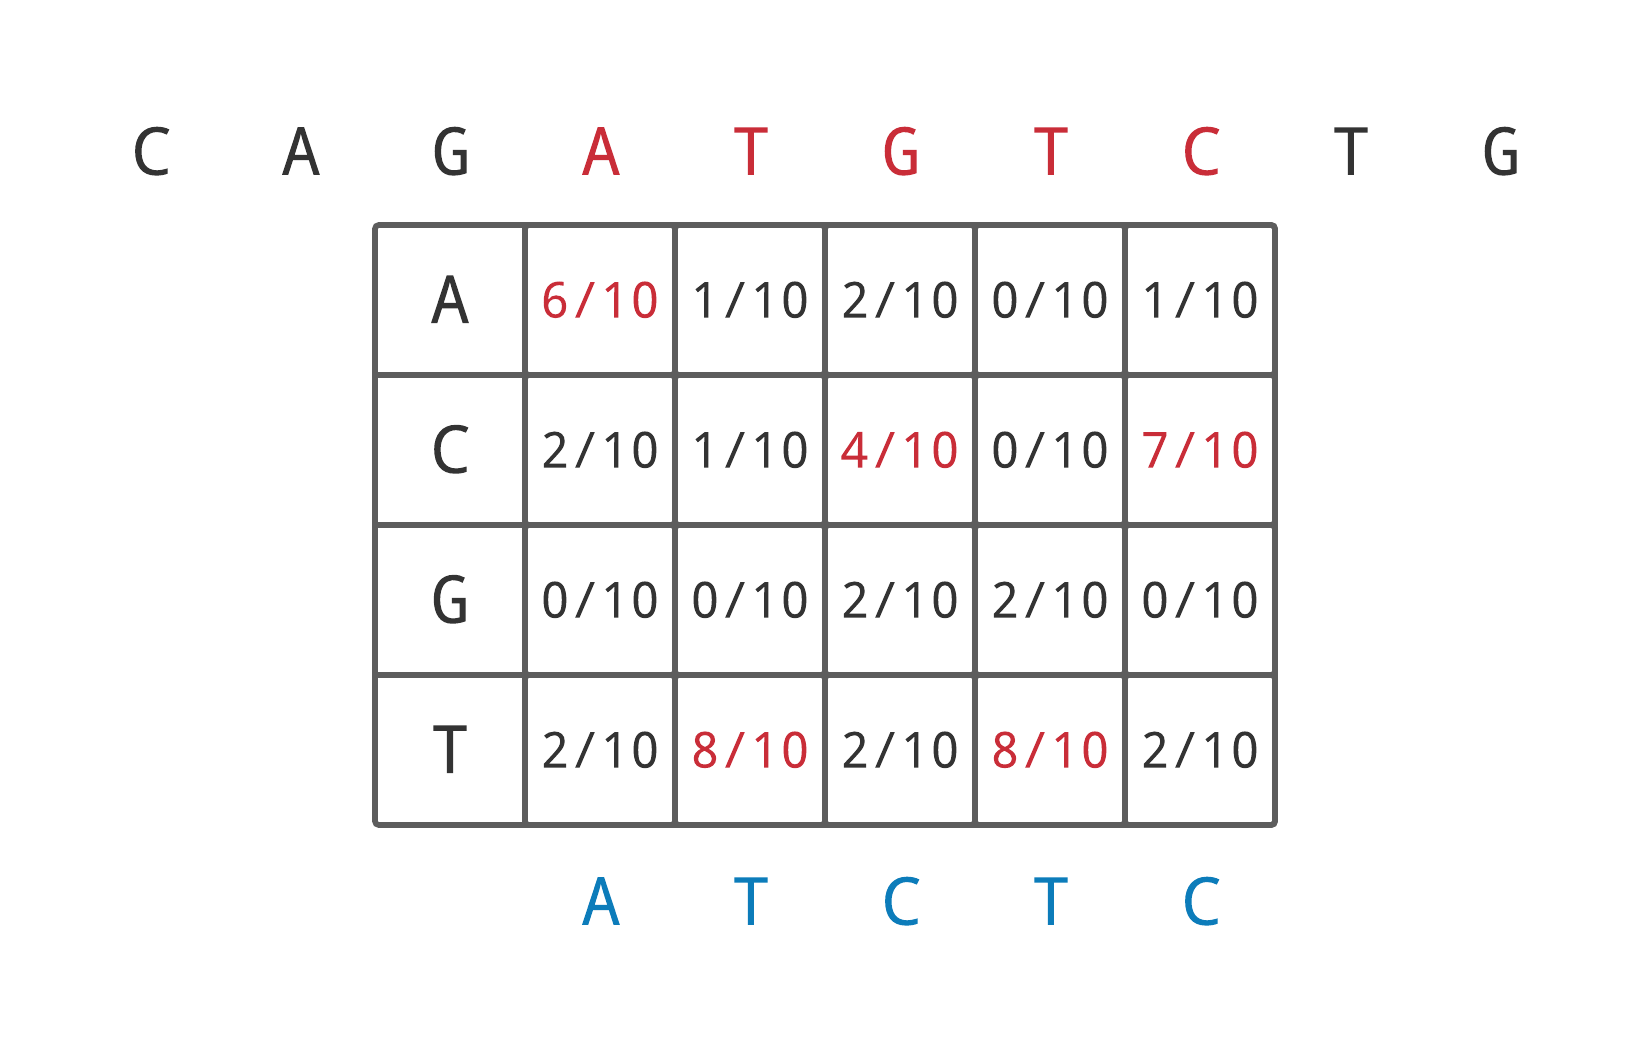
\includegraphics[scale=0.2]{c2/logos/2C.png} 
\end{center}
\hline\vspace{5}

\subsection*{Formatting}
\textbf{Input:} A string \emph{Text}, an integer $k$, and a $4\times k$ matrix \emph{Profile} of floats.\\
\noindent\textbf{Output:} A string representing a \emph{Profile}-most probable $k$-mer in \emph{Text} (If multiple answers exist, you may return any one).

\subsection*{Constraints}
\begin{itemize}
    \item The length of \emph{Text} will be between $1$ and $10^3$.
    \item The integer $k$ will be between $1$ and $10^1$.
    \item \emph{Text} will be a DNA string.
\end{itemize}
\pagebreak

\subsection*{\href{https://github.com/rjeveloff/BA_problemregister/tree/main/test_cases/chapter_2/2C}{Test Cases \gitlogo}}
\stepcounter{subsubsection}\subsubsection*{Case \arabic{subsubsection}}
\hline \vspace{5}
\textbf{Description:} The sample dataset is not actually run on your code.\\ \\
\noindent \textbf{Input:}\\
\code{ACCTGTTTATTGCCTAAGTTCCGAACAAACCCAATATAGCCCGAGGGCCT\\5\\0.2 0.2 0.3 0.2 0.3\\0.4 0.3 0.1 0.5 0.1\\0.3 0.3 0.5 0.2 0.4\\0.1 0.2 0.1 0.1 0.2}\\ \\
\noindent \textbf{Output:}\\
\code{CCGAG}

\stepcounter{subsubsection}\subsubsection*{Case \arabic{subsubsection}}
\hline \vspace{5}
\textbf{Description:} This dataset checks for off-by-one errors at the beginning of \emph{Text}. Notice that the optimal solution (\code{AGCAGCTT}) occurs at the very beginning of \emph{Text}, so if your code does not check this $k$-mer, then your code will output a different (incorrect) $k$-mer as the solution.\\ \\
\noindent \textbf{Input:}\\
\code{AGCAGCTTTGACTGCAACGGGCAATATGTCTCTGTGTGGATTAAAAAAAGAGTGTCTGATCTGAACTGGT\dots\\
\dots TACCTGCCGTGAGTAAAT\\8\\0.7 0.2 0.1 0.5 0.4 0.3 0.2 0.1\\0.2 0.2 0.5 0.4 0.2 0.3 0.1 0.6\\0.1 0.3 0.2 0.1 0.2 0.1 0.4 0.2\\0.0 0.3 0.2 0.0 0.2 0.3 0.3 0.1}\\ \\
\noindent \textbf{Output:}\\
\code{AGCAGCTT}
\pagebreak

\stepcounter{subsubsection}\subsubsection*{Case \arabic{subsubsection}}
\hline \vspace{5}
\textbf{Description:} This dataset checks for off-by-one errors at the end of \emph{Text}. Notice that the optimal solution (\code{AAGCAGAGTTTA}) occurs at the very end of \emph{Text}, so if your code does not check this $k$-mer, then your code will output a different (incorrect) $k$-mer as the solution.\\ \\
\noindent \textbf{Input:}\\
\code{TTACCATGGGACCGCTGACTGATTTCTGGCGTCAGCGTGATGCTGGTGTGGATGACATTCCGGTGCGCTT\dots\\\dots TGTAAGCAGAGTTTA\\12\\0.2 0.3 0.4 0.5 0.6 0.7 0.8 0.1 0.2 0.3 0.4 0.5\\0.3 0.2 0.1 0.1 0.2 0.1 0.1 0.4 0.3 0.2 0.2 0.1\\0.2 0.1 0.4 0.3 0.1 0.1 0.1 0.3 0.1 0.1 0.2 0.1\\0.3 0.4 0.1 0.1 0.1 0.1 0.0 0.2 0.4 0.4 0.2 0.3}\\ \\
\noindent \textbf{Output:}\\
\code{AAGCAGAGTTTA}

\stepcounter{subsubsection}\subsubsection*{Case \arabic{subsubsection}}
\hline \vspace{5}
\textbf{Description:} A larger dataset of the same size as that provided by the randomized autograder. Check input/output folders for this dataset.\\ \\
\pagebreak
%                                                                                                                           PROBLEM BREAK
\subsection{Implement GreedyMotifSearch}
\hline\vspace{5}
\noindent\textbf{Greedy Motif Search Problem}\\
\emph{Implement GreedyMotifSearch}.\\ \\
\textbf{Input:} A collection of strings \emph{Dna}, and integers $k$ and $t$.\\
\textbf{Output:} A collection of strings resulting from running \sc{GreedyMotifSearch}(\emph{Dna}, $k$, $t$).
\begin{center}
    
\includegraphics[scale=0.2]{c2/logos/2D.png} 
\end{center}
\hline\vspace{5}

\subsection*{Formatting}
\textbf{Input:} Space-separated integers $k$ and $t$, followed by a newline-separated collection of strings \emph{Dna}.\\
\noindent\textbf{Output:} A space-separated list of strings resulting from running \sc{GreedyMotifSearch}(\emph{Dna}, $k$, $t$) (If at any step you find more than one \emph{Profile}-most probable $k$-mer in a given string, use the one occurring first).

\subsection*{Constraints}
\begin{itemize}
    \item The integer $k$ will be between $1$ and $10^2$.
    \item The integer $t$ will be between $1$ and $10^2$.
    \item The number of strings in \emph{Dna} will be between $1$ and $10^2$.
    \item The length of each string in \emph{Dna} will be between $1$ and $10^2$.
    \item Each string in \emph{Dna} will be a DNA string.
\end{itemize}
\pagebreak

\subsection*{\href{https://github.com/rjeveloff/BA_problemregister/tree/main/test_cases/chapter_2/2D}{Test Cases \gitlogo}}
\stepcounter{subsubsection}\subsubsection*{Case \arabic{subsubsection}}
\hline \vspace{5}
\textbf{Description:} The sample dataset is not actually run on your code.\\ \\
\noindent \textbf{Input:}\\
\code{3 5\\GGCGTTCAGGCA AAGAATCAGTCA CAAGGAGTTCGC CACGTCAATCAC CAATAATATTCG}\\ \\
\noindent \textbf{Output:}\\
\code{CAG CAG CAA CAA CAA}

\stepcounter{subsubsection}\subsubsection*{Case \arabic{subsubsection}}
\hline \vspace{5}
\textbf{Description:} This dataset checks that your code always picks the first-occurring Profile-most Probable $k$-mer in a given sequence of \emph{Dna}. In the first sequence (\code{GCCCAA}), \code{GCC} and \code{CCA} are both Profile-most Probable $k$-mers. However, you must return \code{GCC} since it occurs earlier than \code{CCA}. Thus, if the first sequence of your output is \code{CCA}, this test case fails your code.\\ \\
\noindent \textbf{Input:}\\
\code{3 4\\GCCCAA GGCCTG AACCTA TTCCTT}\\ \\
\noindent \textbf{Output:}\\
\code{GCC GCC AAC TTC}
\pagebreak

\stepcounter{subsubsection}\subsubsection*{Case \arabic{subsubsection}}
\hline \vspace{5}
\textbf{Description:} This dataset checks if your code has an off-by-one error at the beginning of each sequence of \emph{Dna}. Notice that the first four motifs of the solution occur at the beginning of their respective sequences in \emph{Dna}, so if your code did not check the first $k$-mer in each sequence of 
\emph{Dna}, it would not find these sequences.\\ \\
\noindent \textbf{Input:}\\
\code{5 8\\GAGGCGCACATCATTATCGATAACGATTCGCCGCATTGCC\\TCATCGAATCCGATAACTGACACCTGCTCTGGCACCGCTC\\TCGGCGGTATAGCCAGAAAGCGTAGTGCCAATAATTTCCT\\GAGTCGTGGTGAAGTGTGGGTTATGGGGAAAGGCAGACTG\\GACGGCAACTACGGTTACAACGCAGCAACCGAAGAATATT\\TCTGTTGTTGCTAACACCGTTAAAGGCGGCGACGGCAACT\\AAGCGGCCAACGTAGGCGCGGCTTGGCATCTCGGTGTGTG\\AATTGAAAGGCGCATCTTACTCTTTTCGCTTTCAAAAAAA}\\ \\
\noindent \textbf{Output:}\\
\code{GAGGC TCATC TCGGC GAGTC GCAGC GCGGC GCGGC GCATC}

\stepcounter{subsubsection}\subsubsection*{Case \arabic{subsubsection}}
\hline \vspace{5}
\textbf{Description:} This dataset checks if your code has an off-by-one error at the end of each sequence of \emph{Dna}. Notice that the first two motifs of the solution occur at the end of their respective sequences in \emph{Dna}, so if your code did not check the end $k$-mer in each sequence of \emph{Dna}, it would not find 
these sequences.\\ \\
\noindent \textbf{Input:}\\
\code{6 5\\GCAGGTTAATACCGCGGATCAGCTGAGAAACCGGAATGTGCGT\\CCTGCATGCCCGGTTTGAGGAACATCAGCGAAGAACTGTGCGT\\GCGCCAGTAACCCGTGCCAGTCAGGTTAATGGCAGTAACATTT\\AACCCGTGCCAGTCAGGTTAATGGCAGTAACATTTATGCCTTC\\ATGCCTTCCGCGCCAATTGTTCGTATCGTCGCCACTTCGAGTG}\\ \\
\noindent \textbf{Output:}\\
\code{GTGCGT GTGCGT GCGCCA GTGCCA GCGCCA}
\pagebreak

\stepcounter{subsubsection}\subsubsection*{Case \arabic{subsubsection}}
\hline \vspace{5}
\textbf{Description:} This test dataset checks if your code is correctly breaking ties when calling Profile-most Probable $k$-mer. Specifically, it makes sure that, when you call Profile-most Probable $k$-mer, in the event of a tie, you choose the first-occurring $k$-mer.\\ \\
\noindent \textbf{Input:}\\
\code{5 8\\GACCTACGGTTACAACGCAGCAACCGAAGAATATTGGCAA\\TCATTATCGATAACGATTCGCCGGAGGCCATTGCCGCACA\\GGAGTCTGGTGAAGTGTGGGTTATGGGGCAGACTGGGAAA\\GAATCCGATAACTGACACCTGCTCTGGCACCGCTCTCATC\\AAGCGCGTAGGCGCGGCTTGGCATCTCGGTGTGTGGCCAA\\AATTGAAAGGCGCATCTTACTCTTTTCGCTTAAAATCAAA\\GGTATAGCCAGAAAGCGTAGTTAATTTCGGCTCCTGCCAA\\TCTGTTGTTGCTAACACCGTTAAAGGCGGCGACGGCAACT}\\ \\
\noindent \textbf{Output:}\\
\code{GCAGC TCATT GGAGT TCATC GCATC GCATC GGTAT GCAAC}

\stepcounter{subsubsection}\subsubsection*{Case \arabic{subsubsection}}
\hline \vspace{5}
\textbf{Description:} A larger dataset of the same size as that provided by the randomized autograder. Check input/output folders for this dataset.\\ \\
\pagebreak
%                                                                                                                           PROBLEM BREAK
\subsection{Implement GreedyMotifSearch with Pseudocounts}
\hline\vspace{5}
\noindent\textbf{Greedy Motif Search with Pseudocounts Problem}\\
\emph{Implement GreedyMotifSearch with pseudocounts}.\\ \\
\textbf{Input:} A collection of strings \emph{Dna}, and integers $k$ and $t$.\\
\textbf{Output:} A collection of strings resulting from running \sc{GreedyMotifSearch}(\emph{Dna}, $k$, $t$) with pseudocounts.
\begin{center}
    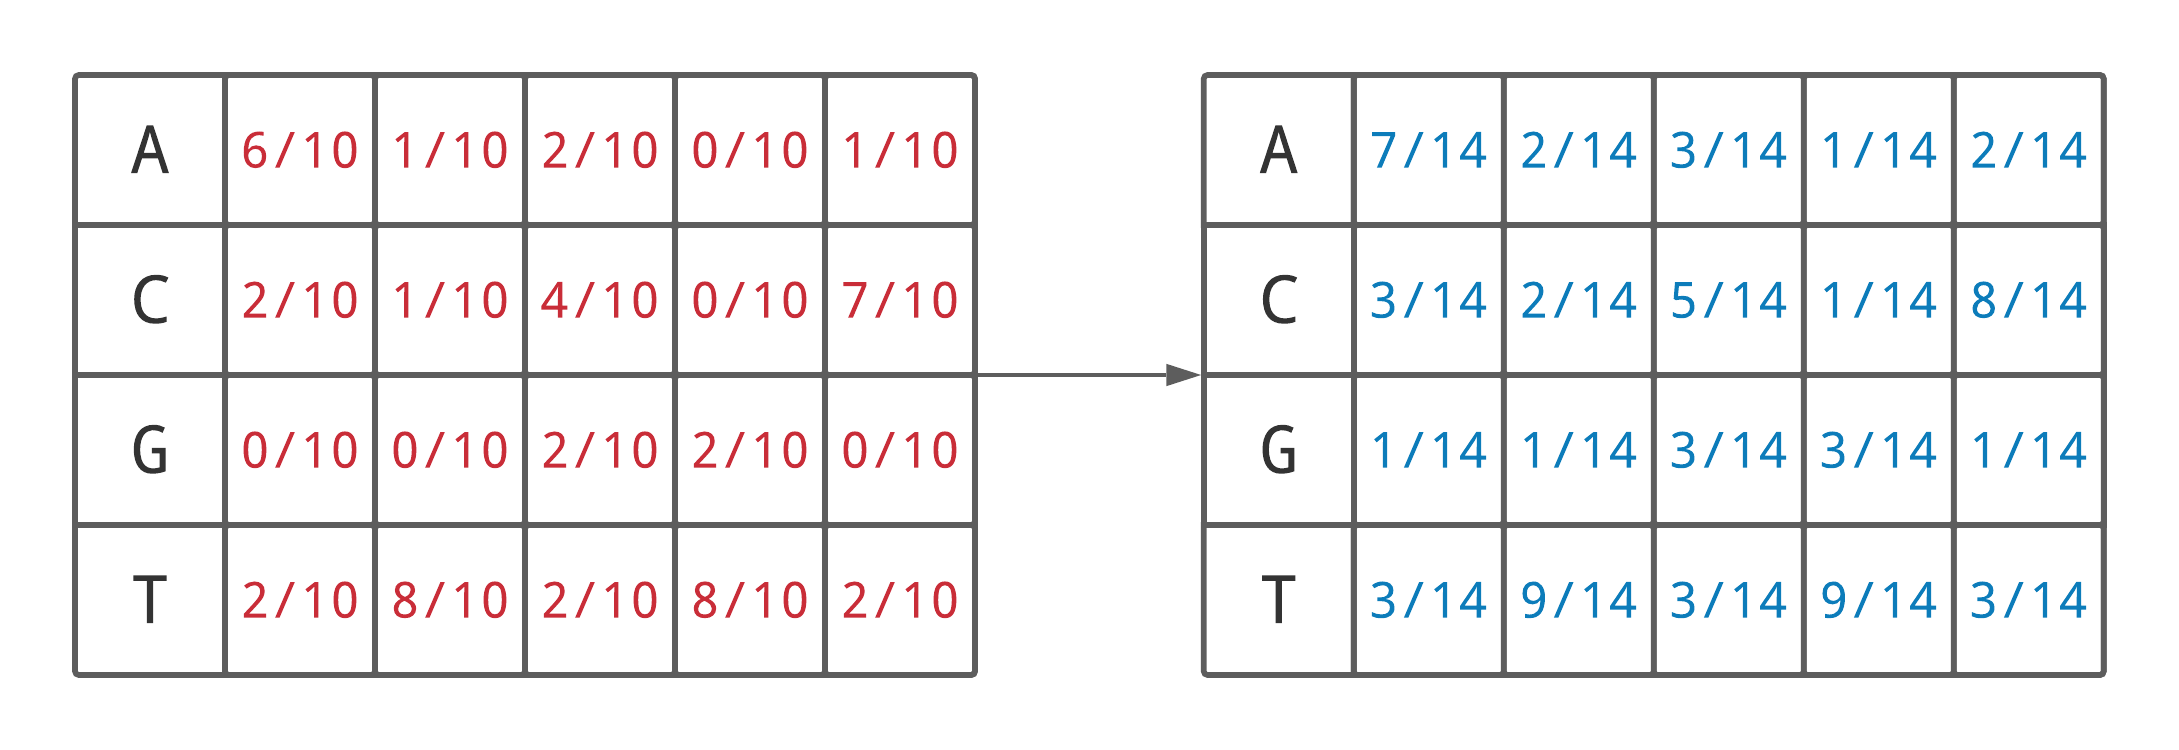
\includegraphics[scale=0.15]{c2/logos/2E.png} 
\end{center}
\hline\vspace{5}

\subsection*{Formatting}
\textbf{Input:} Space-separated integers $k$ and $t$, followed by a newline-separated collection of strings \emph{Dna}.\\
\noindent\textbf{Output:} A space-separated list of strings containing a collection of strings resulting from running \sc{GreedyMotifSearch}(\emph{Dna}, $k$, $t$) with pseudocounts (If at any step you find more than one \emph{Profile}-most probable $k$-mer in a given string, use the one occurring first).

\subsection*{Constraints}
\begin{itemize}
    \item The integer $k$ will be between $1$ and $10^2$.
    \item The integer $t$ will be between $1$ and $10^2$.
    \item The number of strings in \emph{Dna} will be between $1$ and $10^2$.
    \item The length of each string in \emph{Dna} will be between $1$ and $10^2$.
    \item Each string in \emph{Dna} will be a DNA string.
\end{itemize}
\pagebreak

\subsection*{\href{https://github.com/rjeveloff/BA_problemregister/tree/main/test_cases/chapter_2/2E}{Test Cases \gitlogo}}
\stepcounter{subsubsection}\subsubsection*{Case \arabic{subsubsection}}
\hline \vspace{5}
\textbf{Description:} The sample dataset is not actually run on your code.\\ \\
\noindent \textbf{Input:}\\
\code{3 5\\GGCGTTCAGGCA AAGAATCAGTCA CAAGGAGTTCGC CACGTCAATCAC CAATAATATTCG}\\ \\
\noindent \textbf{Output:}\\
\code{TTC ATC TTC ATC TTC}

\stepcounter{subsubsection}\subsubsection*{Case \arabic{subsubsection}}
\hline \vspace{5}
\textbf{Description:} A larger dataset of the same size as that provided by the randomized autograder. Check input/output folders for this dataset.\\ \\
\pagebreak
%                                                                                                                           PROBLEM BREAK
\subsection{Implement RandomizedMotifSearch}
\hline\vspace{5}
\noindent\textbf{Randomized Motif Search Problem}\\
\emph{Implement RandomizedMotifSearch}.\\ \\
\textbf{Input:} A collection of strings \emph{Dna}, and integers $k$ and $t$.\\
\textbf{Output:} A collection of strings resulting from running \sc{RandomizedMotifSearch}(\emph{Dna}, $k$, $t$) 1000 times. Remember to use pseudocounts!
\begin{center}
    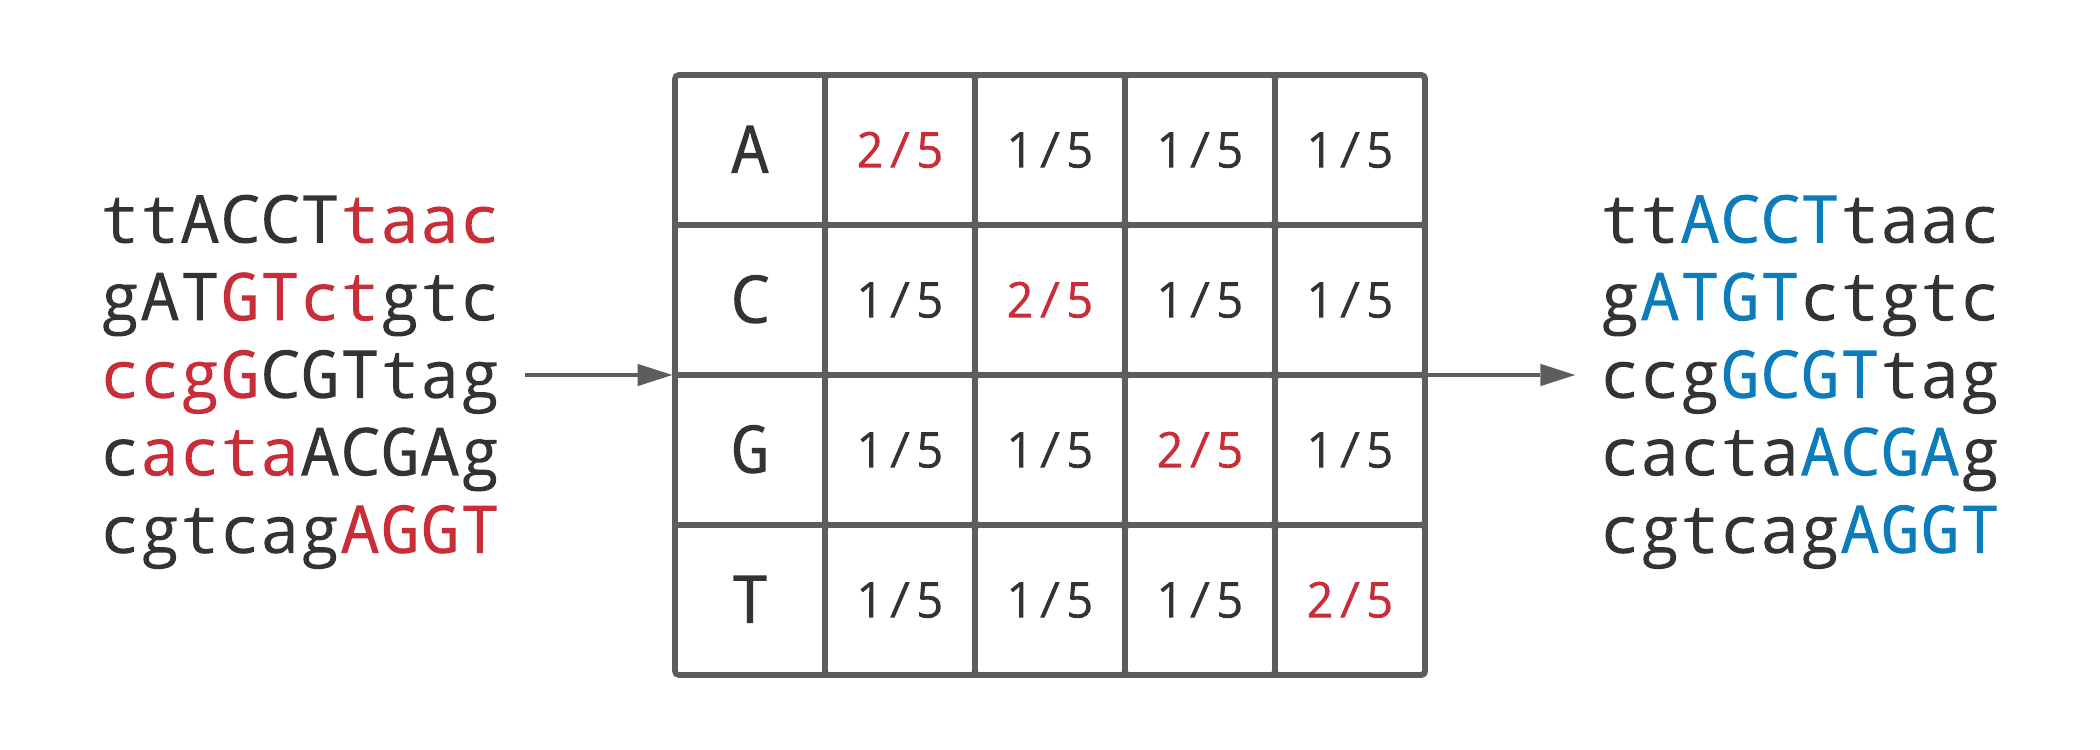
\includegraphics[scale=0.14]{c2/logos/2F.png} 
\end{center}
\hline\vspace{5}

\subsection*{Formatting}
\textbf{Input:} Space-separated integers $k$ and $t$, followed by a newline-separated collection of strings \emph{Dna}.\\
\noindent\textbf{Output:} A space-separated list of strings containing a collection of strings resulting from running \sc{RandomizedMotifSearch}(\emph{Dna}, $k$, $t$) 1000 times. Remember to use pseudocounts!

\subsection*{Constraints}
\begin{itemize}
    \item The integer $k$ will be between $1$ and $10^2$.
    \item The integer $t$ will be between $1$ and $10^2$.
    \item The number of strings in \emph{Dna} will be between $1$ and $10^2$.
    \item The length of each string in \emph{Dna} will be between $1$ and $10^2$.
    \item Each string in \emph{Dna} will be a DNA string.
\end{itemize}
\pagebreak

\subsection*{\href{https://github.com/rjeveloff/BA_problemregister/tree/main/test_cases/chapter_2/2F}{Test Cases \gitlogo}}
\stepcounter{subsubsection}\subsubsection*{Case \arabic{subsubsection}}
\hline \vspace{5}
\textbf{Description:} A small and hand-solvable dataset taken from the example problem on Stepik.\\ \\
\noindent \textbf{Input:}\\
\code{8 5\\CGCCCCTCTCGGGGGTGTTCAGTAAACGGCCA GGGCGAGGTATGTGTAAGTGCCAAGGTGCCAG\\TAGTACCGAGACCGAAAGAAGTATACAGGCGT TAGATCAAGTTTCAGGTGCACGTCGGTGAACC\\AATCCACCAGCTCCACGTGCAATGTTGGCCTA}\\ \\
\noindent \textbf{Output:}\\
\code{TCTCGGGG CCAAGGTG TACAGGCG TTCAGGTG TCCACGTG}

\stepcounter{subsubsection}\subsubsection*{Case \arabic{subsubsection}}
\hline \vspace{5}
\textbf{Description:} This dataset checks if your code has an off-by-one error at the beginning of each sequence of \emph{Dna}. Notice that the some of the motifs of the solution occur at the beginning of their respective sequences in \emph{Dna}, so if your code did not check the first $k$-mer in each sequence of \emph{Dna}, it would not find these sequences.\\ \\
\noindent \textbf{Input:}\\
\code{6 8\\AATTGGCACATCATTATCGATAACGATTCGCCGCATTGCC\\GGTTAACATCGAATAACTGACACCTGCTCTGGCACCGCTC\\AATTGGCGGCGGTATAGCCAGATAGTGCCAATAATTTCCT\\GGTTAATGGTGAAGTGTGGGTTATGGGGAAAGGCAGACTG\\AATTGGACGGCAACTACGGTTACAACGCAGCAAGAATATT\\GGTTAACTGTTGTTGCTAACACCGTTAAGCGACGGCAACT\\AATTGGCCAACGTAGGCGCGGCTTGGCATCTCGGTGTGTG\\GGTTAAAAGGCGCATCTTACTCTTTTCGCTTTCAAAAAAA }\\ \\
\noindent \textbf{Output:}\\
\code{CGATAA GGTTAA GGTATA GGTTAA GGTTAC GGTTAA GGCCAA GGTTAA}
\pagebreak

\stepcounter{subsubsection}\subsubsection*{Case \arabic{subsubsection}}
\hline \vspace{5}
\textbf{Description:} This dataset checks if your code has an off-by-one error at the end of each sequence of \emph{Dna}. Notice that the some of the motifs of the solution occur at the end of their respective sequences in \emph{Dna}, so if your code did not check the last $k$-mer in each sequence of \emph{Dna}, it would not find these sequences.\\ \\
\noindent \textbf{Input:}\\
\code{6 8\\GCACATCATTAAACGATTCGCCGCATTGCCTCGATTAACC\\TCATAACTGACACCTGCTCTGGCACCGCTCATCCAAGGCC\\AAGCGGGTATAGCCAGATAGTGCCAATAATTTCCTTAACC\\AGTCGGTGGTGAAGTGTGGGTTATGGGGAAAGGCAAGGCC\\AACCGGACGGCAACTACGGTTACAACGCAGCAAGTTAACC\\AGGCGTCTGTTGTTGCTAACACCGTTAAGCGACGAAGGCC\\AAGCTTCCAACATCGTCTTGGCATCTCGGTGTGTTTAACC\\AATTGAACATCTTACTCTTTTCGCTTTCAAAAAAAAGGCC}\\ \\
\noindent \textbf{Output:}\\
\code{TTAACC ATAACT TTAACC TGAAGT TTAACC TTAAGC TTAACC TGAACA}

\stepcounter{subsubsection}\subsubsection*{Case \arabic{subsubsection}}
\hline \vspace{5}
\textbf{Description:} A larger dataset of the same size as that provided by the randomized autograder. Check input/output folders for this dataset.\\ \\
\pagebreak
%                                                                                                                           PROBLEM BREAK
\subsection{Implement GibbsSampler}
\hline\vspace{5}
\noindent\textbf{Gibbs Sampler Problem}\\
\emph{Implement GibbsSampler}.\\ \\
\noindent\textbf{Input:} A collection of DNA strings \emph{Dna}, and integers $k$, $t$, and $N$.\\
\noindent\textbf{Output:} The strings resulting from running \sc{GibbsSampler}(\emph{Dna}, $k$, $t$, $N$) with 20 random starts. Remember to use pseudocounts!
\begin{center}
    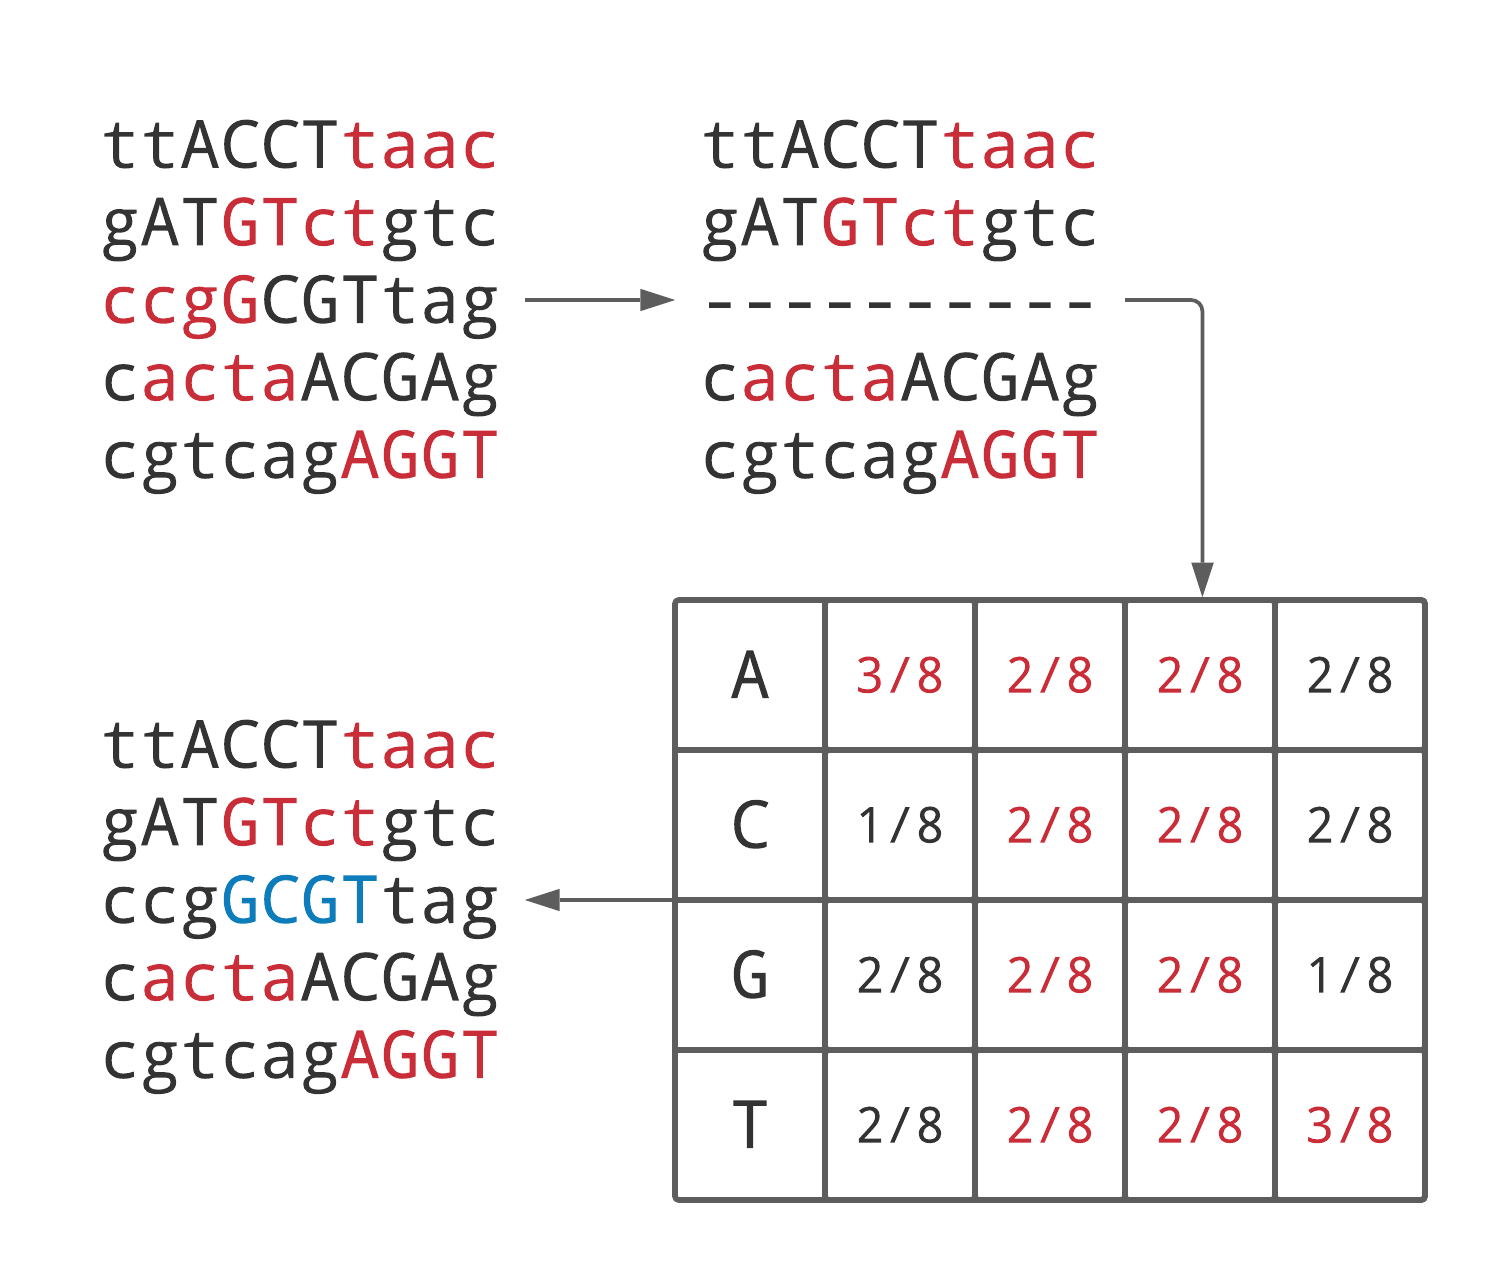
\includegraphics[scale=0.15]{c2/logos/2G.png} 
\end{center}
\hline\vspace{5}

\subsection*{Formatting}
\noindent\textbf{Input:} Space-separated integers $k$, $t$, and $N$, followed by a newline-separated collection of DNA strings \emph{Dna}.\\
\noindent\textbf{Output:} A space-separated list of strings containing the strings resulting from running \sc{GibbsSampler}(\emph{Dna}, $k$, $t$, $N$) with 20 random starts. Remember to use pseudocounts!

\subsection*{Constraints}
\begin{itemize}
    \item The integer $k$ will be between $1$ and $10^2$.
    \item The integer $t$ will be between $1$ and $10^2$.
    \item The integer $N$ will be between $1$ and $10^4$.
    \item The number of strings in \emph{Dna} will be between $1$ and $10^2$.
    \item The length of each string in \emph{Dna} will be between $1$ and $10^3$.
    \item Each string in \emph{Dna} will be a DNA string.
\end{itemize}
\pagebreak

\subsection*{\href{https://github.com/rjeveloff/BA_problemregister/tree/main/test_cases/chapter_2/2G}{Test Cases \gitlogo}}
\stepcounter{subsubsection}\subsubsection*{Case \arabic{subsubsection}}
\hline \vspace{5}
\textbf{Description:} The sample dataset is not actually run on your code.\\ \\
\noindent \textbf{Input:}\\
\code{8 5 100\\CGCCCCTCTCGGGGGTGTTCAGTAAACGGCCA GGGCGAGGTATGTGTAAGTGCCAAGGTGCCAG\\TAGTACCGAGACCGAAAGAAGTATACAGGCGT TAGATCAAGTTTCAGGTGCACGTCGGTGAACC\\AATCCACCAGCTCCACGTGCAATGTTGGCCTA}\\ \\
\noindent \textbf{Output:}\\
\code{TCTCGGGG CCAAGGTG TACAGGCG TTCAGGTG TCCACGTG}

\stepcounter{subsubsection}\subsubsection*{Case \arabic{subsubsection}}
\hline \vspace{5}
\textbf{Description:} A larger dataset of the same size as that provided by the randomized autograder. Check input/output folders for this dataset.\\ \\
\pagebreak
%                                                                                                                           PROBLEM BREAK
\subsection{Implement DistanceBetweenPatternAndStrings}
\hline\vspace{5}
\noindent\textbf{Distance Between Pattern and Strings Problem}\\
\emph{Compute DistanceBetweenPatternAndStrings}.\\ \\
\noindent\textbf{Input:} A DNA string \emph{Pattern} and a collection of DNA strings \emph{Dna}.\\
\noindent\textbf{Output:} Distance \sc{d}(\emph{Pattern}, \emph{Dna}) between \emph{Pattern} and \emph{Dna}.
\begin{center}
    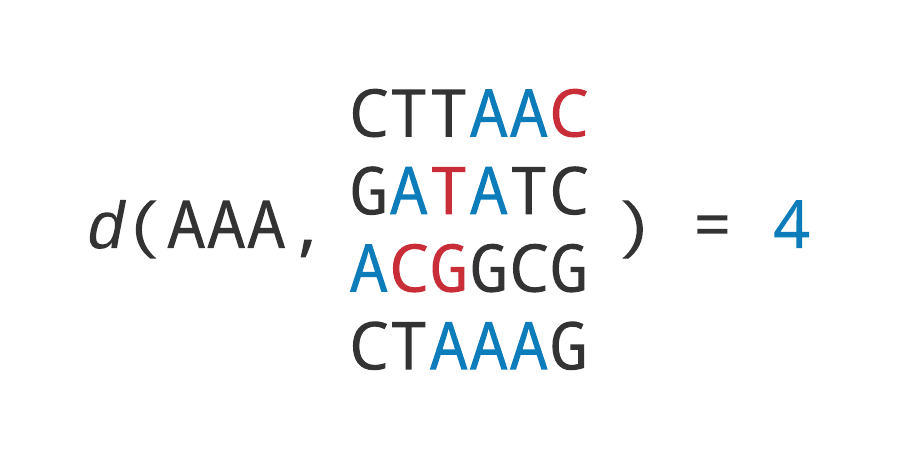
\includegraphics[scale=0.24]{c2/logos/2H.png} 
\end{center}
\hline\vspace{5}

\subsection*{Formatting}
\noindent\textbf{Input:} A DNA string \emph{Pattern}, followed by a space-separated collection of DNA strings \emph{Dna}.\\
\noindent\textbf{Output:} An integer representing the output of \sc{DistanceBetweenPatternAndStrings}(\emph{Pattern}, \emph{Dna}).

\subsection*{Constraints}
\begin{itemize}
    \item The length of \emph{Pattern} will be between $1$ and $10^1$.
    \item The number of strings in \emph{Dna} will be between $1$ and $10^2$.
    \item The length of each string in \emph{Dna} will be between $1$ and $10^2$.
    \item \emph{Pattern} and each string in \emph{Dna} will be DNA strings.
\end{itemize}
\pagebreak

\subsection*{\href{https://github.com/rjeveloff/BA_problemregister/tree/main/test_cases/chapter_2/2H}{Test Cases \gitlogo}}
\stepcounter{subsubsection}\subsubsection*{Case \arabic{subsubsection}}
\hline \vspace{5}
\textbf{Description:} The sample dataset is not actually run on your code.\\ \\
\noindent \textbf{Input:}\\
\code{AAA\\TTACCTTAAC GATATCTGTC ACGGCGTTCG CCCTAAAGAG CGTCAGAGGT}\\ \\
\noindent \textbf{Output:}\\
\code{5}

\stepcounter{subsubsection}\subsubsection*{Case \arabic{subsubsection}}
\hline \vspace{5}
\textbf{Description:} This dataset checks multiple potential mistakes. First, it checks that you are actually using all three sequences of \emph{Dna} (and not just a single sequence). The Hamming Distance between \emph{Pattern} and each individual sequence in \emph{Dna} is $1$, so if your code returns a total score of $1$, we fail it for this reason. Next, it checks if you are only using the first $k$-mer in each sequence of Dna. For example, if you do this, you would output $d$(\code{TAA},\code{TTT})$+d$(\code{TAA},\code{CCT})$+d$(\code{TAA},\code{GGT}) which is $8$, instead of the correct answer of $3$. Finally, it checks if you are only using the last $k$-mer in each sequence of \emph{Dna}. For example, if you do this, you would output $d$(\code{TAA},\code{TTT})$+d$(\code{TAA},\code{CAC})$+d$(\code{TAA},\code{GAG}) which is $6$, instead of the correct answer of $3$.\\ \\
\noindent \textbf{Input:}\\
\code{TAA\\TTTATTT CCTACAC GGTAGAG}\\ \\
\noindent \textbf{Output:}\\
\code{3}

\stepcounter{subsubsection}\subsubsection*{Case \arabic{subsubsection}}
\hline \vspace{5}
\textbf{Description:} This dataset checks if your code is using maximum or sum instead of minimum. First, it checks if your code is using maximum instead of minimum. In this case, the output would be $d$(\code{AAA},\code{ACT})$+d$(\code{AAA},\code{AAC})$+d$(\code{AAA},\code{AAG}), which is $4$, instead of the correct answer of $0$. Next, it checks if your code is using sum instead of minimum. In this case, the output would be 
$d$(\code{AAA},\code{AAA})$+d$(\code{AAA},\code{AAC})$+d$(\code{AAA},\code{ACT})$+d$(\code{AAA},\code{AAA})$+d$(\code{AAA},\code{AAC})$+d$(\code{AAA},\code{AAA})$+d$(\code{AAA},\code{AAG}), which is $5$, instead of the correct answer of $0$.\\ \\
\noindent \textbf{Input:}\\
\code{AAA\\AAACT AAAC AAAG}\\ \\
\noindent \textbf{Output:}\\
\code{0}
\pagebreak

\stepcounter{subsubsection}\subsubsection*{Case \arabic{subsubsection}}
\hline \vspace{5}
\textbf{Description:} This dataset checks if your code has an off-by-one error at the end of each sequence of \emph{Dna}. Notice that each sequence has a perfect match of \code{AAA} at the very end, so if your code returns a nonzero answer to this test dataset, it must have missed the last $k$-mer of each.\\ \\
\noindent \textbf{Input:}\\
\code{AAA\\TTTTAAA CCCCAAA GGGGAAA}\\ \\
\noindent \textbf{Output:}\\
\code{0}

\stepcounter{subsubsection}\subsubsection*{Case \arabic{subsubsection}}
\hline \vspace{5}
\textbf{Description:} A larger dataset of the same size as that provided by the randomized autograder. Check input/output folders for this dataset.\\ \\
\pagebreak
%                                                                                                                           PROBLEM BREAK
\section{How Do We Assemble Genomes?\\ \normalfont{\emph{Graph Algorithms}}}
\begin{center}
    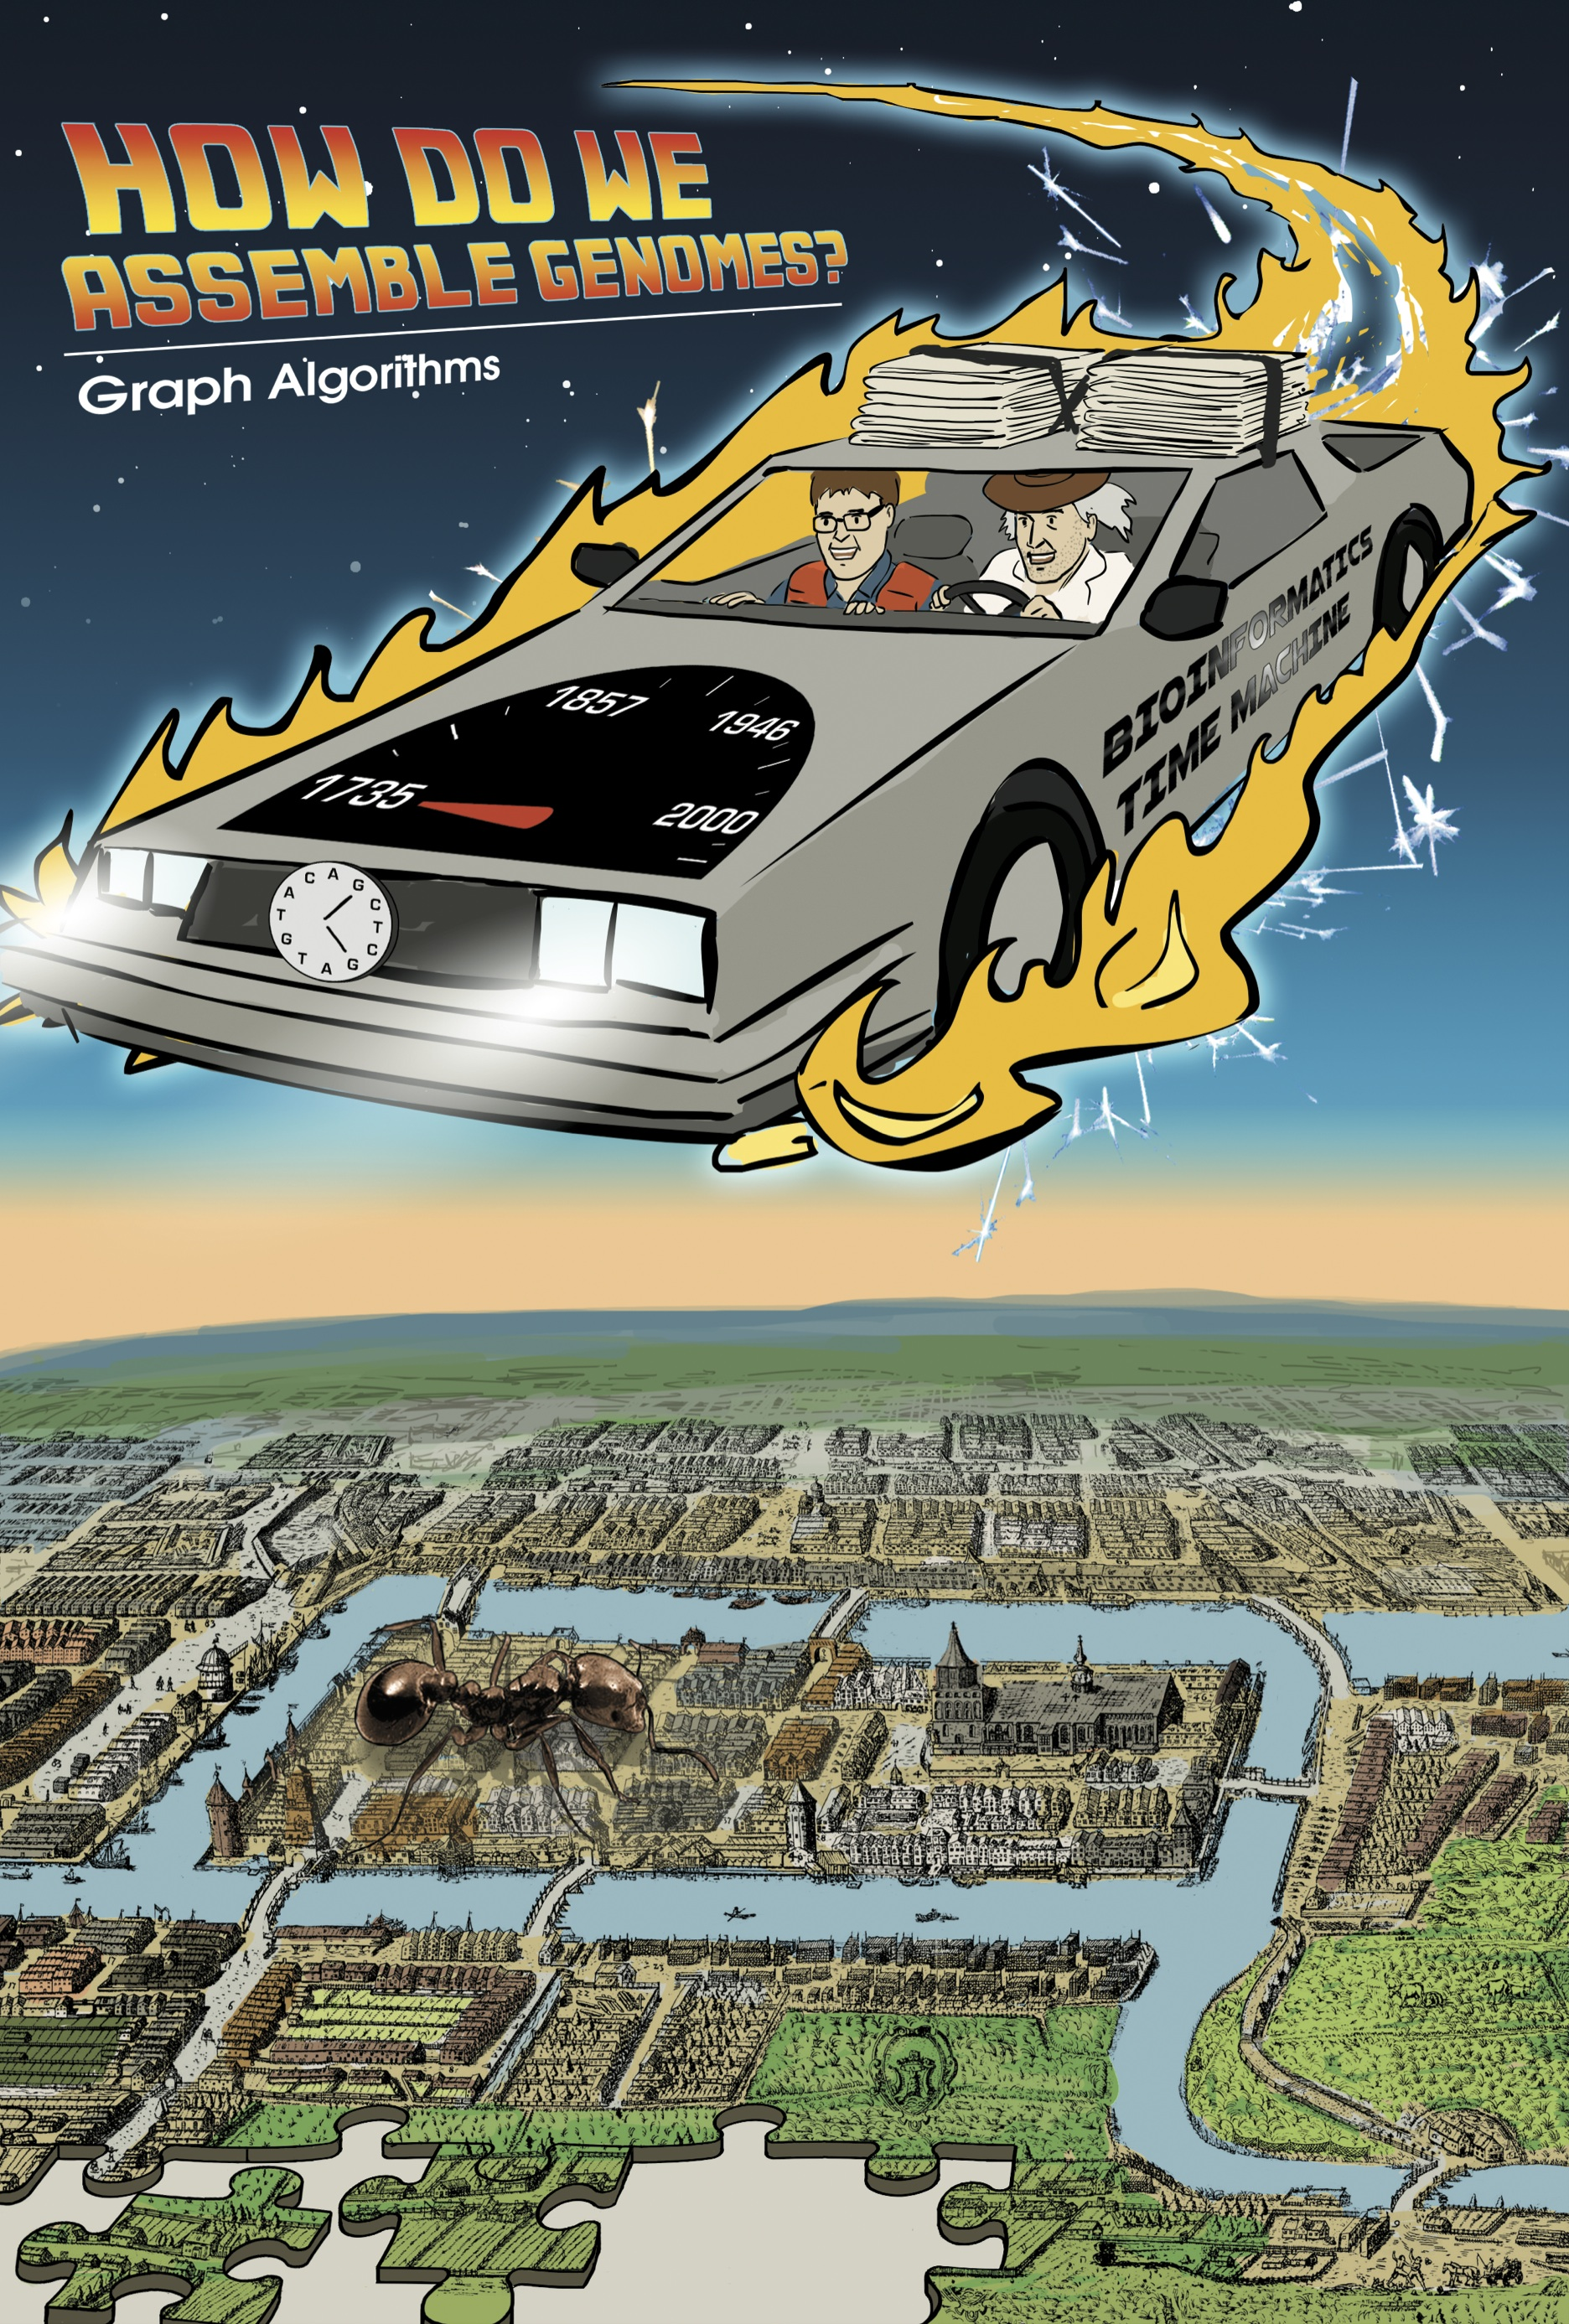
\includegraphics[scale=0.72]{c3/c3.jpg}
\end{center}
\pagebreak

\subsection{Generate the $k$-mer Composition of a String}
\hline\vspace{5}
\textbf{String Composition Problem}\\
\emph{Generate the $k$-mer composition of a string}.\\ \\
\textbf{Input:} An integer $k$ and a string \emph{Text}.\\
\textbf{Output:} The collection of $k$-mers \sc{Composition}$_k$(\emph{Text}).
\begin{center}
    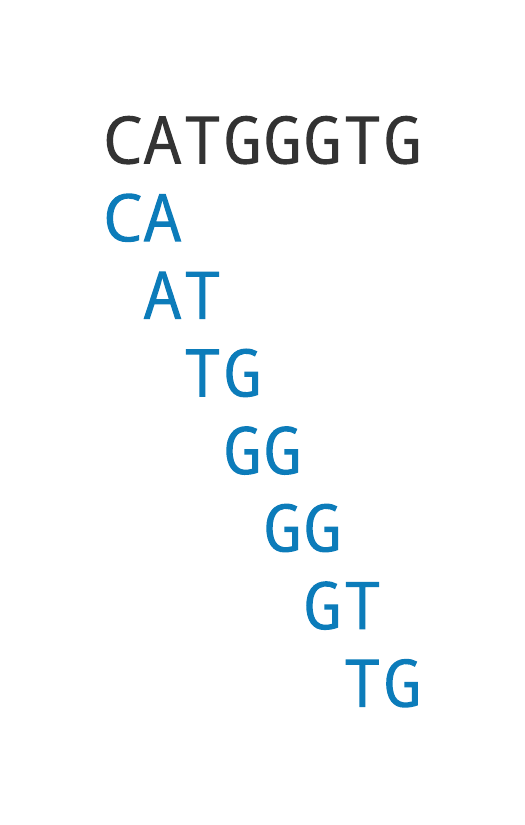
\includegraphics[scale=0.24]{c3/logos/3A.png}
\end{center}
\hline\vspace{5}

\subsection*{Formatting}
\noindent\textbf{Input:} A integer $k$ followed by a string \emph{Text}.\\
\noindent\textbf{Output:} A space-separated list of $k$-mer strings representing \sc{Composition}$_k$(\emph{Text}) (the $k$-mers can be provided in any order).

\subsection*{Constraints}
\begin{itemize}
    \item The value of $k$ will be between $1$ and $10^3$.
    \item The length \emph{Text} will be between $1$ and $10^4$.
    \item No pattern is a prefix of another pattern.
\end{itemize}
\pagebreak

\subsection{Reconstruct a String from its Genome Path}
\hline\vspace{5}
\textbf{String Spelled by a Genome Path Problem}\\
\emph{Find the string spelled by a genome path}.\\ \\
\textbf{Input:} A sequence of $k$-mers \emph{Pattern}$_1$, ... , \emph{Pattern}$_n$ such that the last $k-1$ symbols of \emph{Pattern}$_i$ are equal to the first $k-1$ symbols of \emph{Pattern}$_i+1$ for $i$ from $1$ to $n-1$.\\
\textbf{Output:} A string \emph{Text} of length $k+n-1$ where the $i$-th $k$-mer in \emph{Text} is equal to \emph{Pattern}$_i$ for all $i$ from $1$ to $n$.
\begin{center}
    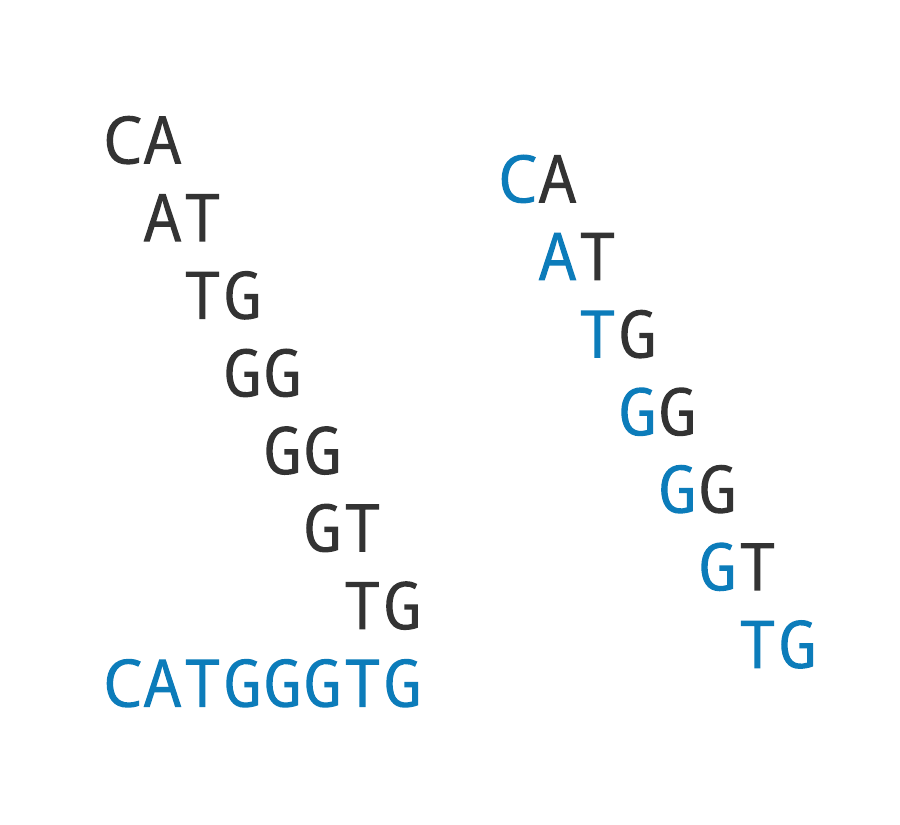
\includegraphics[scale=0.24]{c3/logos/3B.png}
\end{center}
\hline\vspace{5}

\subsection*{Formatting}
\noindent\textbf{Input:} A space-separated list of strings \emph{Patterns}.\\
\noindent\textbf{Output:} A string \emph{Text}.

\subsection*{Constraints}
\begin{itemize}
    \item The number of patterns in the string-set \emph{Pattern} will be between $1$ and $10^4$.
    \item The length of any one pattern in \emph{Pattern} will be between $1$ and $10^2$.
\end{itemize}
\pagebreak

\subsection{Construct the Overlap Graph of a Collection of $k$-mers}
\hline\vspace{5}
\textbf{Overlap Graph Problem}\\
\emph{Construct the overlap graph of a collection of $k$-mers}.\\ \\
\textbf{Input:} A collection \emph{Patterns} of $k$-mers.\\
\textbf{Output:} The overlap graph of \emph{Patterns}.
\begin{center}
    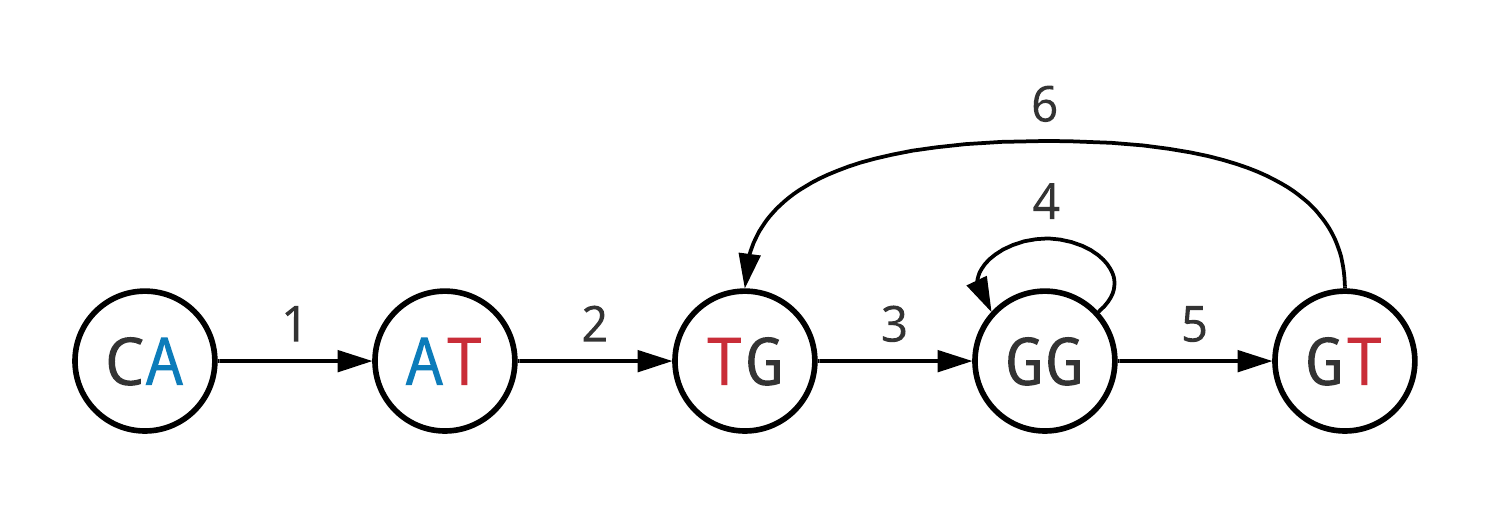
\includegraphics[scale=0.24]{c3/logos/3C.png}
\end{center}
\hline\vspace{5}

\subsection*{Formatting}
\noindent\textbf{Input:} A space-separated list of strings \emph{Patterns}.\\
\noindent\textbf{Output:} An adjacency list representing the overlap graph of \emph{Patterns}.

\subsection*{Constraints}
\begin{itemize}
    \item The number of patterns in the string-set \emph{Patterns} will be between $1$ and $10^3$.
    \item The length of any one pattern in \emph{Patterns} will be between $1$ and $10^2$.
\end{itemize}
\pagebreak

\subsection{Construct the De Bruijn Graph of a String}
\hline\vspace{5}
\textbf{De Bruijn Graph from a String Problem}\\
\emph{Construct the de Bruijn graph of a string}.\\ \\
\textbf{Input:} An integer $k$ and a string \emph{Text}.\\
\textbf{Output:} The graph \sc{DeBruijn}$_k$(\emph{Text}).
\begin{center}
    \includegraphics[scale=0.2]{c3/logos/3D.png}
\end{center}
\hline\vspace{5}

\subsection*{Formatting}
\noindent\textbf{Input:} A integer $k$ followed by a string \emph{Text}.\\
\noindent\textbf{Output:} \sc{DeBruijn}$_k$(\emph{Text}), in the form of an adjacency list.

\subsection*{Constraints}
\begin{itemize}
    \item The value of $k$ will be between $1$ and $10^2$.
    \item The length of \emph{Text} will be between $1$ and $10^4$.
\end{itemize}
\pagebreak

\subsection{Construct the De Bruijn Graph of a Collection of $k$-mers}
\hline\vspace{5}
\textbf{De Bruijn Graph from $k$-mers Problem}\\
\emph{Construct the de Bruijn graph from a collection of $k$-mers}.\\ \\
\textbf{Input:} A collection of $k$-mers \emph{Patterns}.\\
\textbf{Output:} The graph \sc{DeBruijn}(\emph{Patterns}).
\begin{center}
    \includegraphics[scale=0.2]{c3/logos/3E.png}
\end{center}
\hline\vspace{5}

\subsection*{Formatting}
\noindent\textbf{Input:} A space-separated list of $k$-mer strings \emph{Patterns}.\\
\noindent\textbf{Output:} An adjacency list representing \sc{DeBruijn}(\emph{Patterns}).

\subsection*{Constraints}
\begin{itemize}
    \item The number of patterns in the string-set \emph{Patterns} will be between $1$ and $10^4$.
    \item The length of any one pattern in \emph{Patterns} will be between $1$ and $10^2$.
    \item All strings in \emph{Patterns} will be DNA strings.
\end{itemize}
\pagebreak

\subsection{Find an Eulerian Cycle in a Graph}
\hline\vspace{5}
\textbf{Eulerian Cycle Problem}\\
\emph{Find an Eulerian cycle in a graph}.\\ \\
\textbf{Input:} An Eulerian directed graph.\\
\textbf{Output:} An Eulerian cycle in this graph.
\begin{center}
    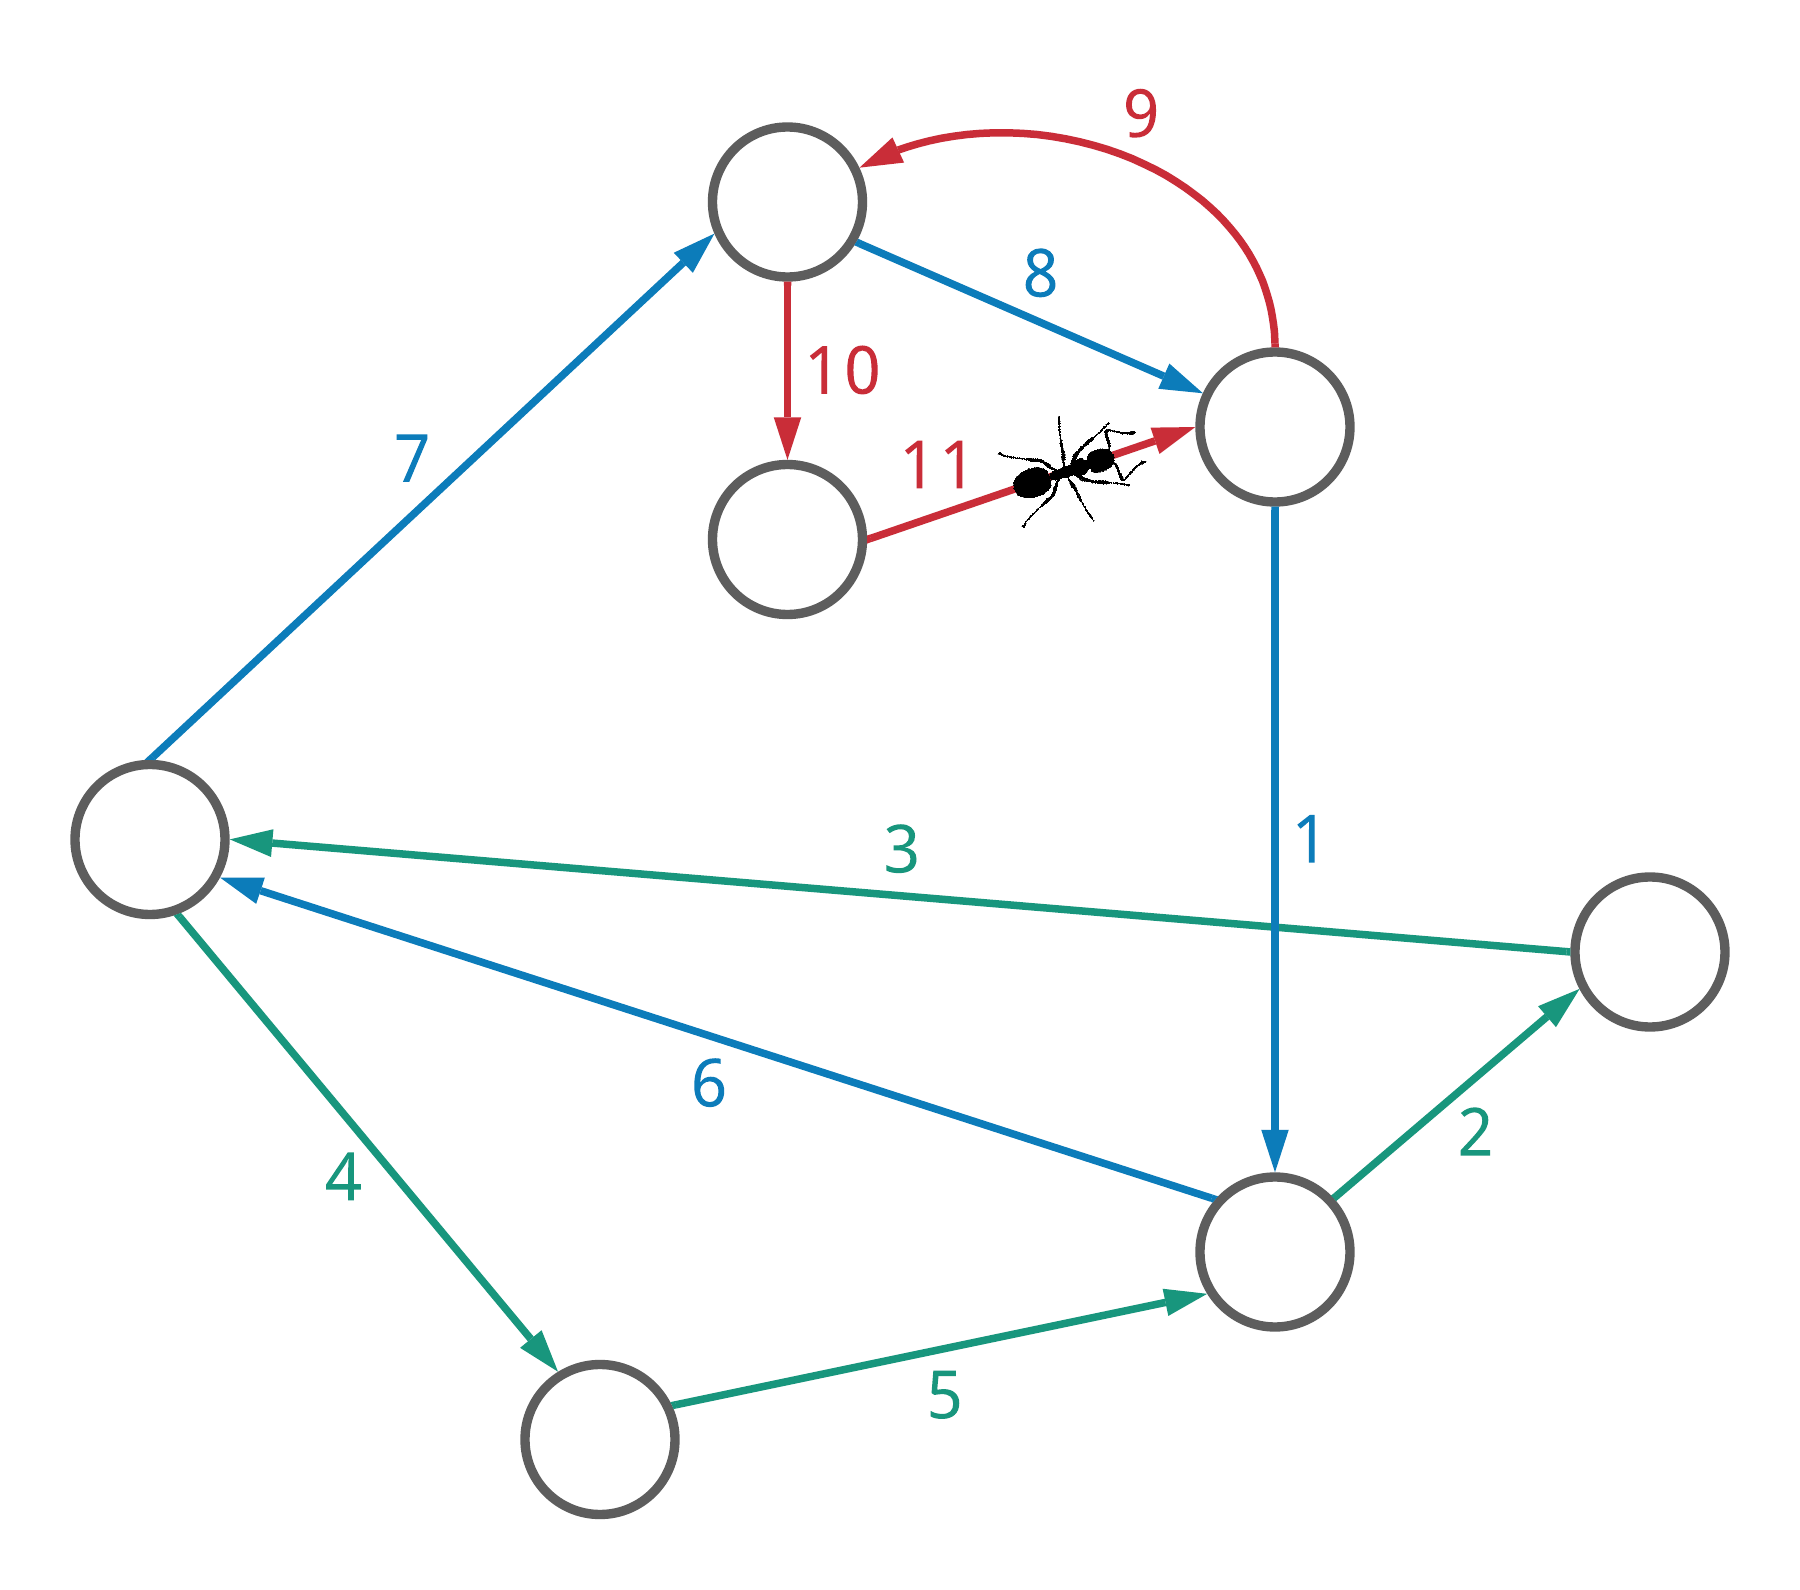
\includegraphics[scale=0.12]{c3/logos/3F.png}
\end{center}
\hline\vspace{5}

\subsection*{Formatting}
\noindent\textbf{Input:} An adjacency list representing an Eulerian directed graph.\\
\noindent\textbf{Output:} A space-separated list of integers representing an Eulerian cycle in the directed graph.

\subsection*{Constraints}
\begin{itemize}
    \item The number of nodes in the graph will be between $1$ and $10^4$.
    \item The number of edges in the graph will be between $1$ and $10^4$.
    \item All nodes in the graph will be labeled with integers.
\end{itemize}
\pagebreak

\subsection{Find an Eulerian Path in a Graph}
\hline\vspace{5}
\textbf{Eulerian Path Problem}\\
\emph{Find an Eulerian path in a graph}.\\ \\
\textbf{Input:} A directed graph containing an Eulerian path.\\
\textbf{Output:} An Eulerian path in this graph.
\begin{center}
    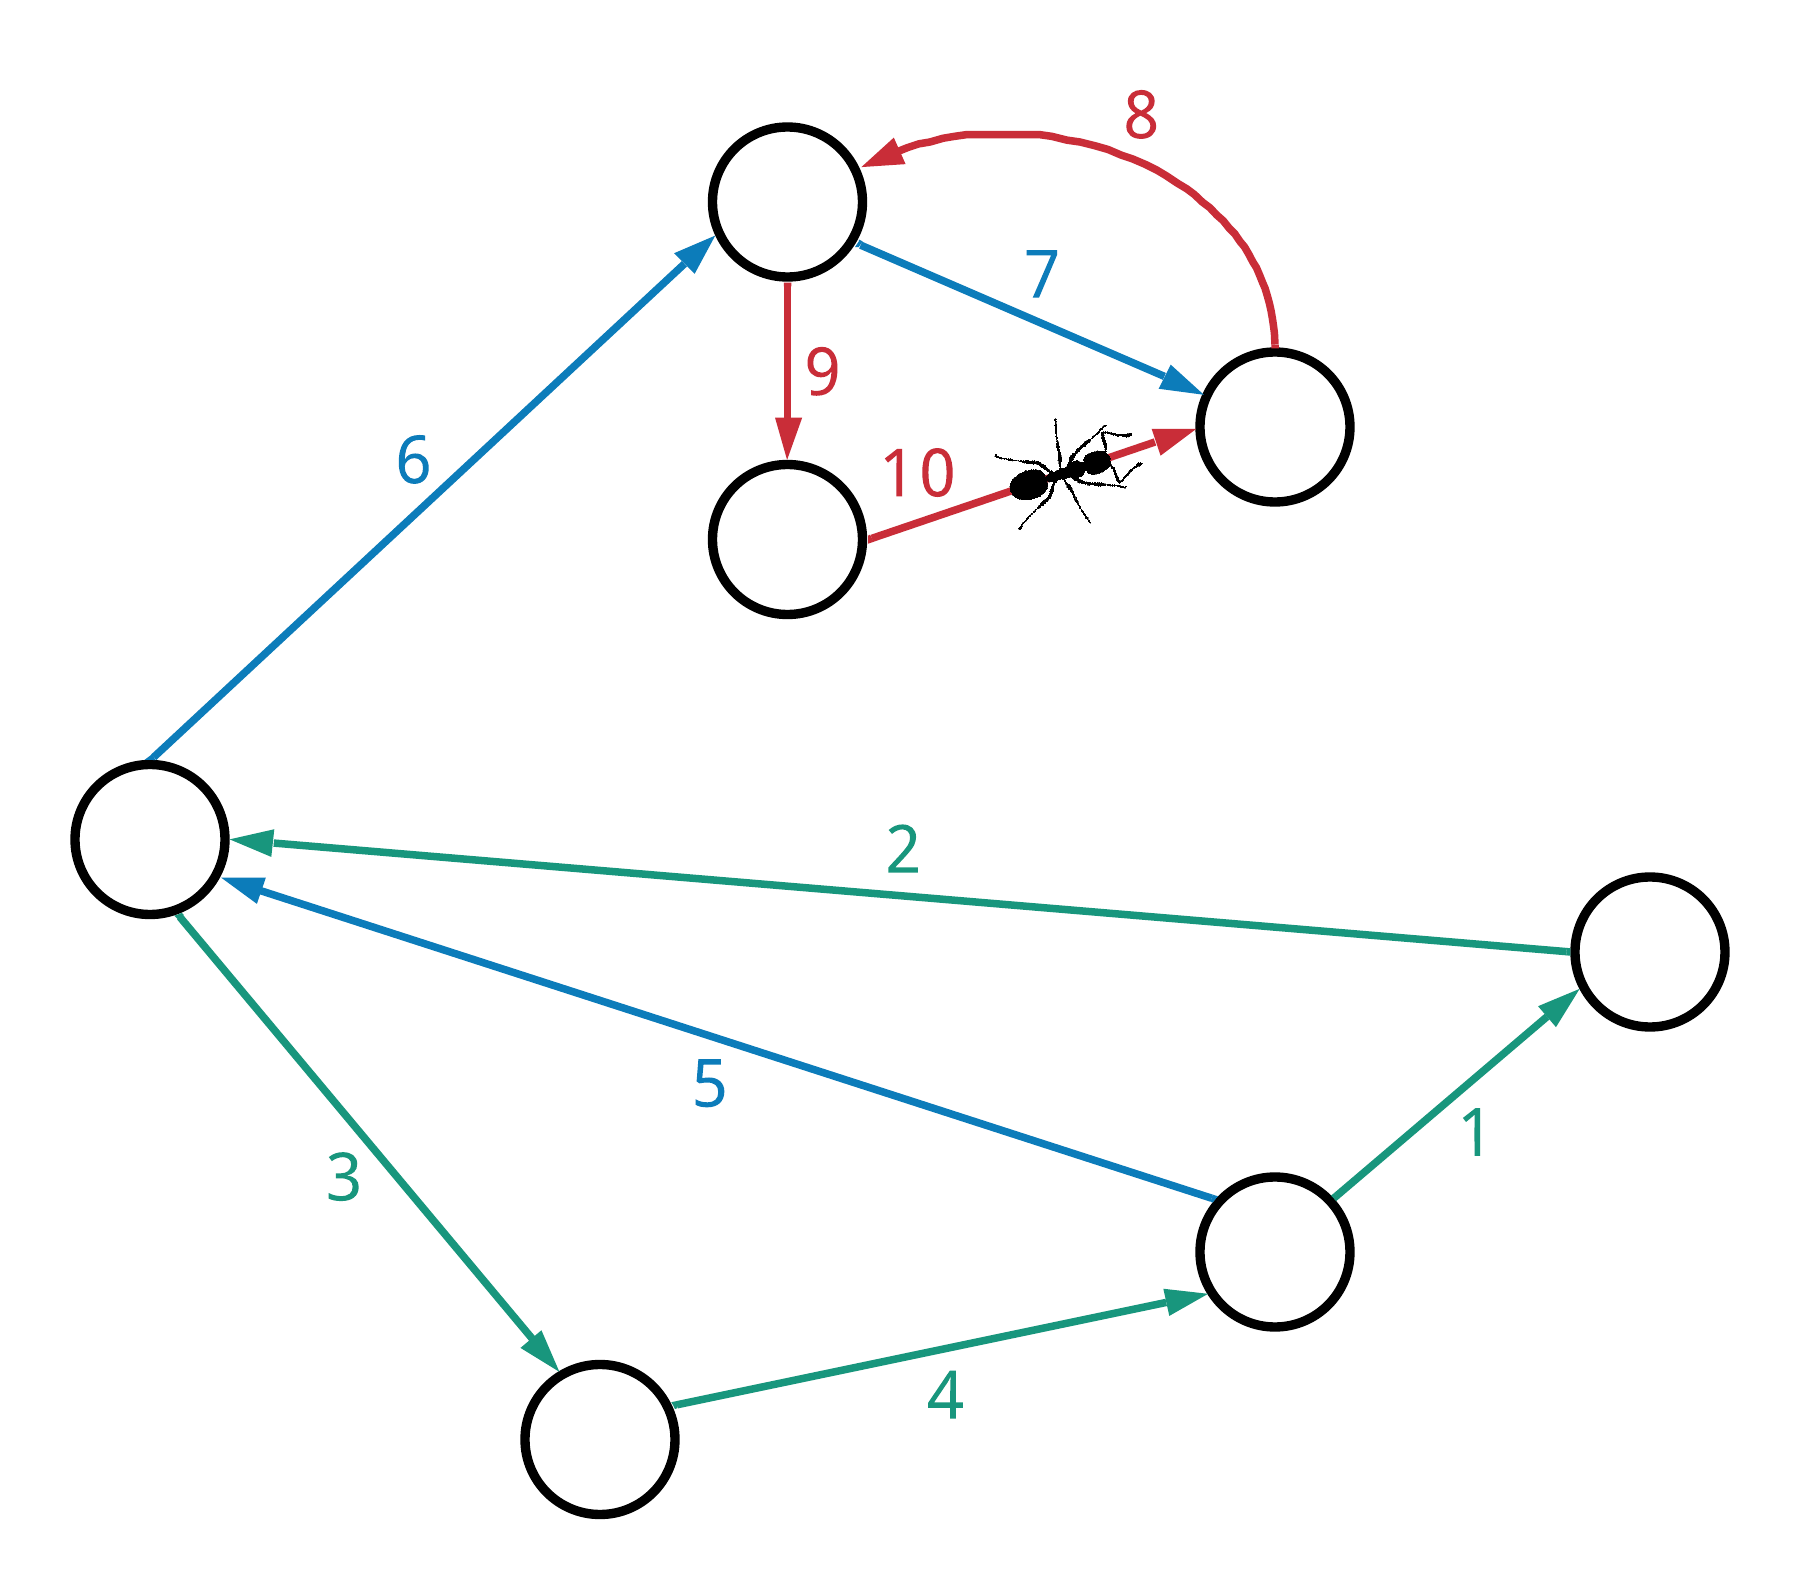
\includegraphics[scale=0.12]{c3/logos/3G.png}
\end{center}
\hline\vspace{5}

\subsection*{Formatting}
\noindent\textbf{Input:} An adjacency list representing a directed graph containing an Eulerian path.\\
\noindent\textbf{Output:} A space-separated list of integers representing an Eulerian path in the graph.

\subsection*{Constraints}
\begin{itemize}
    \item The number of nodes in the graph will be between $1$ and $10^4$.
    \item The number of edges in the graph will be between $1$ and $10^4$.
    \item All nodes in the graph will be labeled with integers.
\end{itemize}
\pagebreak

\subsection{Reconstruct a String from its $k$-mer Composition}
\hline\vspace{5}
\textbf{String Reconstruction Problem}\\
\emph{Reconstruct a string from its $k$-mer composition}.\\ \\
\textbf{Input:} An integer $k$ and a collection of $k$-mers \emph{Patterns}.\\
\textbf{Output:} A string \emph{Text} with $k$-mer composition equal to \emph{Patterns}.
\begin{center}
    \includegraphics[scale=0.2]{c3/logos/3H.png}
\end{center}
\hline\vspace{5}

\subsection*{Formatting}
\noindent\textbf{Input:} An integer $k$ followed by a space-separated list of $k$-mer strings \emph{Patterns}.\\
\noindent\textbf{Output:} A string \emph{Text} with $k$-mer composition equal to \emph{Patterns} (if multiple answers exist, you may return any one).

\subsection*{Constraints}
\begin{itemize}
    \item The value of $k$ will be between $1$ and $10^2$.
    \item The number of strings in \emph{Patterns} will be between $1$ and $10^4$.
    \item The length of any one pattern in \emph{Pattern} will be between $1$ and $10^2$.
\end{itemize}
\pagebreak

\subsection{Find a $k$-Universal Circular String}
\hline\vspace{5}
\textbf{$k$-Universal Circular String Problem}\\
\emph{Find a $k$-universal circular binary string}.\\ \\
\textbf{Input:} An integer $k$.\\
\textbf{Output:} A $k$-universal circular binary string.
\begin{center}
    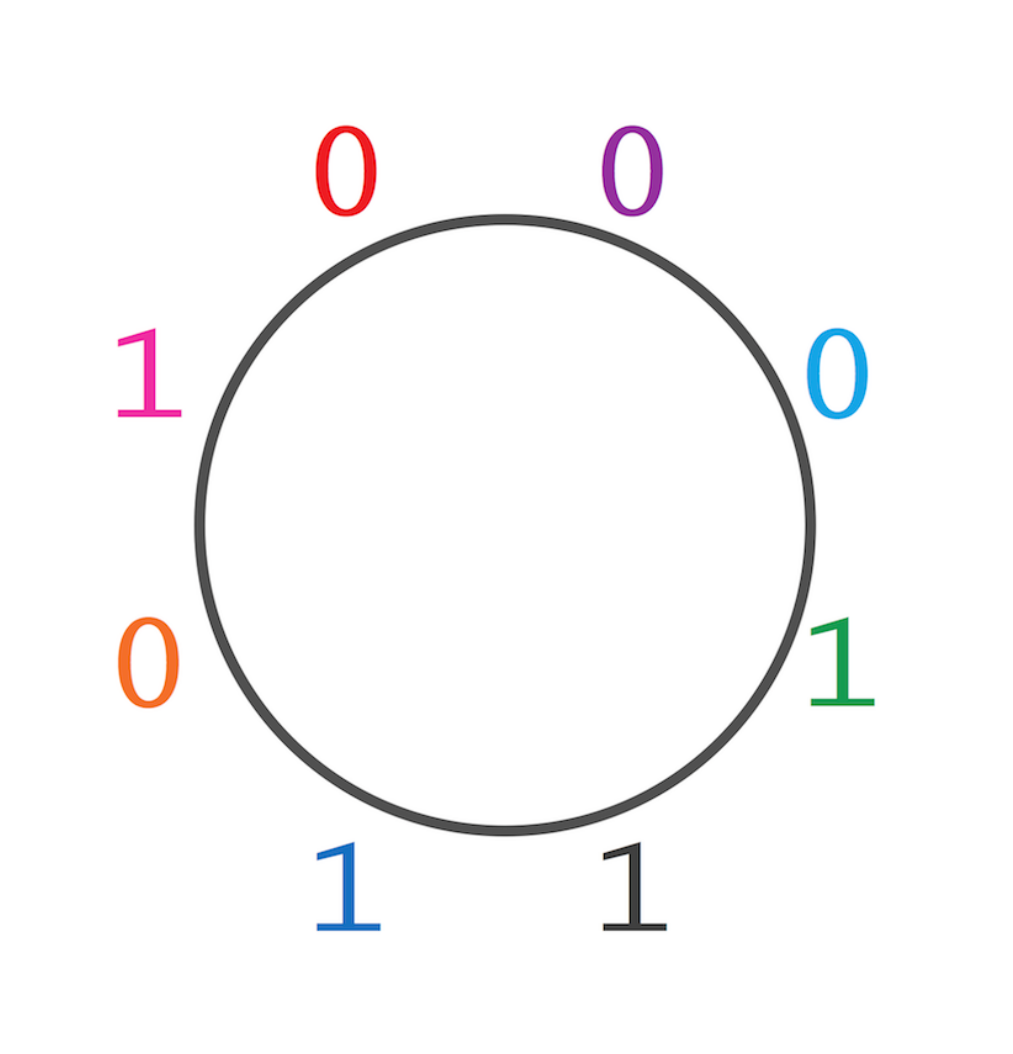
\includegraphics[scale=0.16]{c3/logos/3I.png}
\end{center}
\hline\vspace{5}

\subsection*{Formatting}
\noindent\textbf{Input:} An integer $k$.\\
\noindent\textbf{Output:} A binary string representing a $k$-universal circular string.

\subsection*{Constraints}
\begin{itemize}
    \item The value of $k$ will be between $1$ and $10^1$.
\end{itemize}
\pagebreak

\subsection{Reconstruct a String from its Paired Composition}
\hline\vspace{5}
\textbf{String Reconstruction from Read-Pairs Problem}\\
\emph{Reconstruct a string from its paired composition}.\\ \\
\textbf{Input:} Integers $k$ and $d$ and a collection of paired $k$-mers \emph{PairedReads}.\\
\textbf{Output:} A string \emph{Text} with ($k$,$d$)-mer composition equal to \emph{PairedReads}.
\begin{center}
    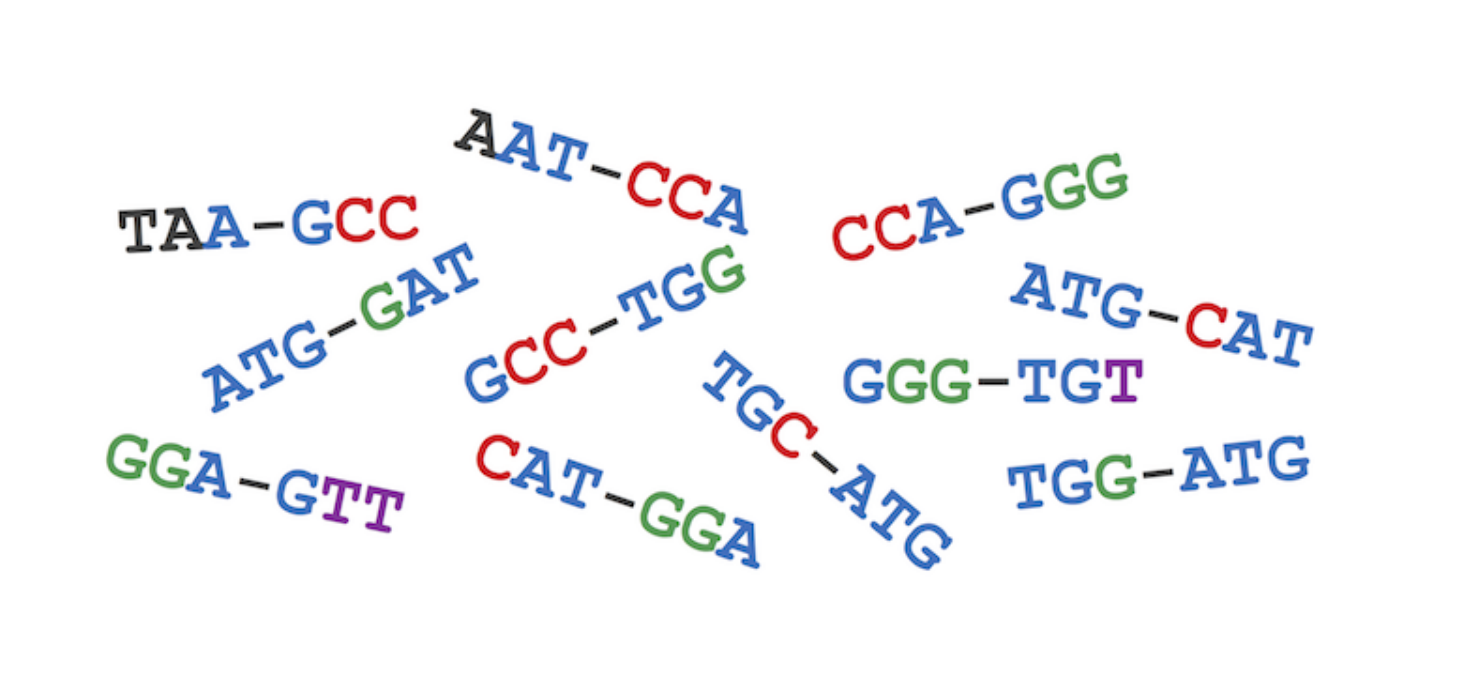
\includegraphics[scale=0.2]{c3/logos/3J.png}
\end{center}
\hline\vspace{5}

\subsection*{Formatting}
\noindent\textbf{Input:} Space-separated integers $k$ and $d$ followed by a space-separated list of paired $k$-mer strings \emph{PairedReads} where individual $k$-mers within the pair are separated by a "|" character.\\
\noindent\textbf{Output:} A string \emph{Text} with ($k$,$d$)-mer composition equal to \emph{PairedReads} (if multiple answers exist, you may return any one).

\subsection*{Constraints}
\begin{itemize}
    \item The value of $k$ will be between $1$ and $10^2$.
    \item The value of $d$ will be between $1$ and $10^3$.
    \item The number of strings in \emph{PairedReads} will be between $1$ and $10^4$.
    \item The length of any one pair of paired $k$-mers in \emph{PairedReads} will be between $1$ and $10^2$.
    \item All $k$-mer strings in \emph{PairedReads} will be DNA strings.
\end{itemize}
\pagebreak

\subsection{Generate Contigs from a Collection of Reads}
\hline\vspace{5}
\textbf{Contig Generation Problem}\\
\emph{Generate the contigs from a collection of reads (with imperfect coverage)}.\\ \\
\textbf{Input:} A collection of $k$-mers \emph{Patterns}.\\
\textbf{Output:} All contigs in the graph \sc{DeBruijn}(\emph{Patterns}).
\begin{center}
    \includegraphics[scale=0.2]{c3/logos/3K.png}
\end{center}
\hline\vspace{5}

\subsection*{Formatting}
\noindent\textbf{Input:} A space-separated list of $k$-mer strings \emph{Patterns}.\\
\noindent\textbf{Output:} A space-separated list of strings representing all contigs in the graph \sc{DeBruijn}(\emph{Patterns}) (you may return the strings in any order).

\subsection*{Constraints}
\begin{itemize}
    \item The number of strings in \emph{Patterns} will be between $1$ and $10^4$.
    \item The length of any given string in \emph{Patterns} will be between $1$ and $10^2$.
\end{itemize}
\pagebreak

\subsection{Construct a String Spelled by a Gapped Genome Path}
\hline\vspace{5}
\textbf{Gapped Genome Path String Problem}\\
\emph{Reconstruct a string from a sequence of ($k$,$d$)-mers corresponding to a path in a paired de Bruijn graph}.\\ \\
\textbf{Input:} A collection of ($k$, $d$)-mers ($a_1$|$b_1$), ... , ($a_n$|$b_n$) such that \sc{Suffix}($a_i$|$b_i$) = \sc{Prefix}($a_{i+1}$|$b_{i+1}$) for all $i$ from $1$ to $n-1$, \emph{PairedReads}.\\
\textbf{Output:} A string \emph{Text} where the $i$-th $k$-mer in \emph{Text} is equal to \sc{Suffix}($a_i$|$b_i$) for all $i$ from $1$ to $n$, if such a string exists.
\begin{center}
    \includegraphics[scale=0.2]{c3/logos/3L.png}
\end{center}
\hline\vspace{5}

\subsection*{Formatting}
\noindent\textbf{Input:} Space-separated integers $k$ and $d$ followed by a space-separated list of paired $k$-mer strings \emph{PairedReads} where individual $k$-mers within the pair are separated by a "|" character.\\
\noindent\textbf{Output:} A string \emph{Text} where the $i$-th $k$-mer in \emph{Text} is equal to \sc{Suffix}($a_i$|$b_i$) for all $i$ from $1$ to $n$, if such a string exists.

\subsection*{Constraints}
\begin{itemize}
    \item The value of $k$ will be between $1$ and $10^2$.
    \item The value of $d$ will be between $1$ and $10^3$.
    \item The number of strings in \emph{PairedReads} will be between $1$ and $10^4$.
    \item The length of any one pair of paired $k$-mers in \emph{PairedReads} will be between $1$ and $10^2$.
    \item All $k$-mer strings in \emph{PairedReads} will be DNA strings.
\end{itemize}
\pagebreak

\subsection{Generate All Maximal Non-Branching Paths in a Graph}
\hline\vspace{5}
\textbf{Maximal Non-Branching Path Problem}\\
\emph{Find all maximal non-branching paths in a graph}.\\ \\
\textbf{Input:} A directed graph.\\
\textbf{Output:} The collection of all maximal non-branching paths in this graph.
\begin{center}
    \includegraphics[scale=0.2]{c3/logos/3M.png}
\end{center}
\hline\vspace{5}

\subsection*{Formatting}
\noindent\textbf{Input:} An adjacency list representing a directed graph.\\
\noindent\textbf{Output:} A newline-separated collection of all maximal non-branching path in the graph where each maximal non-branching path is represented as a space-separated list of integer node labels.

\subsection*{Constraints}
\begin{itemize}
    \item The number of nodes in the graph will be between $1$ and $10^3$.
    \item The number of edges in the graph will be between $1$ and $10^3$.
    \item All nodes in the graph will be labeled with integers.
\end{itemize}
\pagebreak

% REMOVE
\stepcounter{section}
%

\section{How Do We Compare DNA Sequences?\\ \normalfont{\emph{Dynamic Programming}}}
\begin{center}
    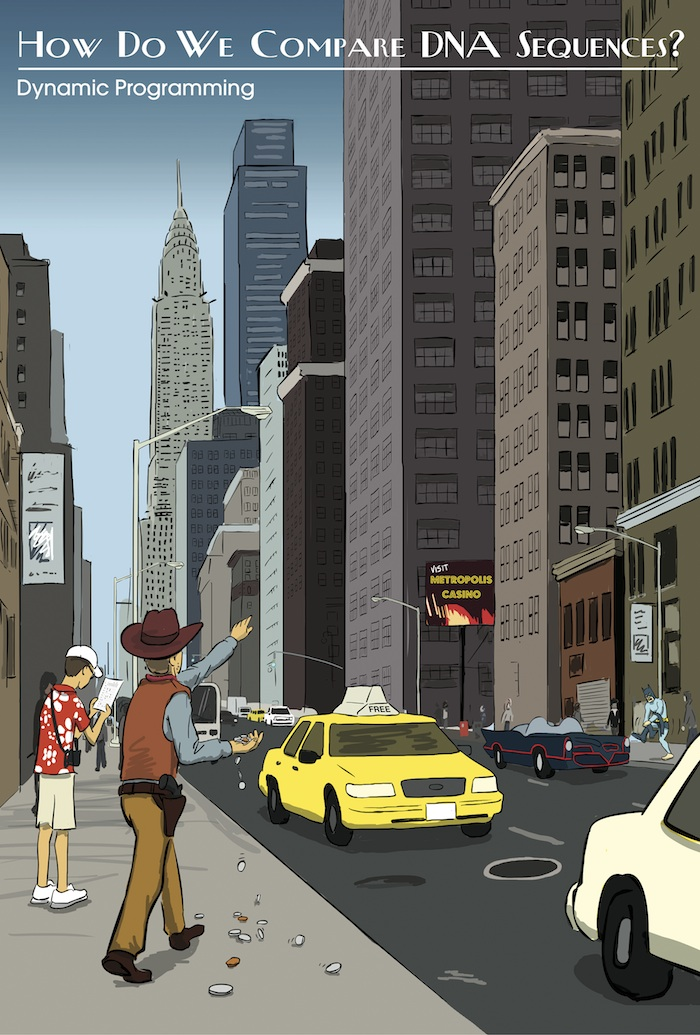
\includegraphics[scale=1.92]{c5/c5.jpg}
\end{center}
\pagebreak

\subsection{Find the Minimum Number of Coins Needed to Make Change}
\hline\vspace{5}
\textbf{The Change Problem}\\
\emph{Find the minimum number of coins needed to make change}.\\ \\
\textbf{Input:} A non-negative integer \emph{money} and an array \emph{Coins} of positive integers.\\
\textbf{Output:} The minimum number of coins with denominations \emph{Coins} that changes \emph{money}.
\begin{center}
    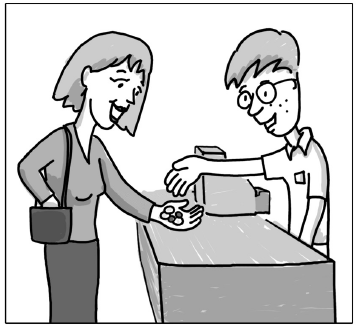
\includegraphics[scale=0.6]{c5/logos/5A.png}
\end{center}
\hline\vspace{5}

\subsection*{Formatting}
\noindent\textbf{Input:} A non-negative integer \emph{money} followed by a space-separated list of positive integers \emph{Coins}.\\
\noindent\textbf{Output:} The minimum number of coins with denominations \emph{Coins} that changes \emph{money}.

\subsection*{Constraints}
\begin{itemize}
    \item The value of \emph{money} will be between $1$ and $10^5$.
    \item The number of positive integers in \emph{Coins} will be between $1$ and $10^1$.
\end{itemize}
\pagebreak

\subsection*{\href{https://github.com/rjeveloff/BA_problemregister/tree/main/test_cases/chapter_5/5A}{Test Cases \gitlogo}}
\stepcounter{subsubsection}\subsubsection*{Case \arabic{subsubsection}}
\hline \vspace{5}
\textbf{Description:} The sample dataset is not actually run on your code.\\ \\
\noindent \textbf{Input:}\\
\code{7\\1 5}\\ \\
\noindent \textbf{Output:}\\
\code{3}

\stepcounter{subsubsection}\subsubsection*{Case \arabic{subsubsection}}
\hline \vspace{5}
\textbf{Description:} This dataset makes sure that your code is correctly considering the last coin denomination in the \emph{Coins} array. If your solution has an off-by-one indexing mistake while iterating over the \emph{Coins} array it could be possible that the last \emph{coin} is not considered. In this case code run on this dataset will output \code{2} instead of the correct answer, \code{1}. \\ \\
\noindent \textbf{Input:}\\
\code{10\\1 2 3 4 5 10}\\ \\
\noindent \textbf{Output:}\\
\code{1}

\stepcounter{subsubsection}\subsubsection*{Case \arabic{subsubsection}}
\hline \vspace{5}
\textbf{Description:} This dataset makes sure that your code is correctly considering the first coin denomination in the \emph{Coins} array. If your solution has an off-by-one indexing mistake while iterating over the \emph{Coins} array it could be possible that the first \emph{coin} is not considered. In this case code run on this dataset will output \code{2} instead of the correct answer, \code{1}.\\ \\
\noindent \textbf{Input:}\\
\code{10\\10 5 4 3 2 1}\\ \\
\noindent \textbf{Output:}\\
\code{1}
\pagebreak

\stepcounter{subsubsection}\subsubsection*{Case \arabic{subsubsection}}
\hline \vspace{5}
\textbf{Description:} This dataset checks if your code correctly returns the final value in the array in the dynamic programming approach for solving this problem. It is possible that an off-by-one indexing error (could be related to confusing $0$/$1$ indexing) results in your code outputting the minimum number of coins needed to make change for \emph{money}$-1$ instead of \emph{money}. In this case your code will output \code{2} instead of the correct value of \emph{3}.\\ \\
\noindent \textbf{Input:}\\
\code{11\\1 5}\\ \\
\noindent \textbf{Output:}\\
\code{3}

\stepcounter{subsubsection}\subsubsection*{Case \arabic{subsubsection}}
\hline \vspace{5}
\textbf{Description:} This dataset checks to make sure you are not using a greedy algorithm to solve this problem. While a greedy algorithm in which the largest valued \emph{coin} is used on each iteration may work in some cases, it will fail on this dataset. A greedy approach would start by using the $9$ \emph{coin} which would only allow for the use of $3$ of the $1$ \emph{coin} to get to $12$, resulting in an output of \code{4}. Using $2$ of the $6$ \emph{coin} will result in exact change with only $2$ coins.\\ \\
\noindent \textbf{Input:}\\
\code{12\\9 6 1}\\ \\
\noindent \textbf{Output:}\\
\code{2}

\stepcounter{subsubsection}\subsubsection*{Case \arabic{subsubsection}}
\hline \vspace{5}
\textbf{Description:} A larger dataset of the same size as that provided by the randomized autograder. Check input/output folders for this dataset.\\ \\
\pagebreak

\subsection{Find the Length of a Longest Path in a Manhattan-like Grid}
\hline\vspace{5}
\textbf{Length of a Longest Path in the Manhattan Tourist Problem}\\
\emph{Find the length of a longest path in a rectangular city}.\\ \\
\textbf{Input:} Integers $n$ and $m$, an $n\times(m+1)$ matrix \emph{Down}, and an $(n+1)\times m$ matrix \emph{Right}.\\
\textbf{Output:} The length of a longest path from source ($0$,$0$) to sink ($n$,$m$) in the $n\times m$ rectangular grid whose edges are defined by the matrices \emph{Down} and \emph{Right}.
\begin{center}
    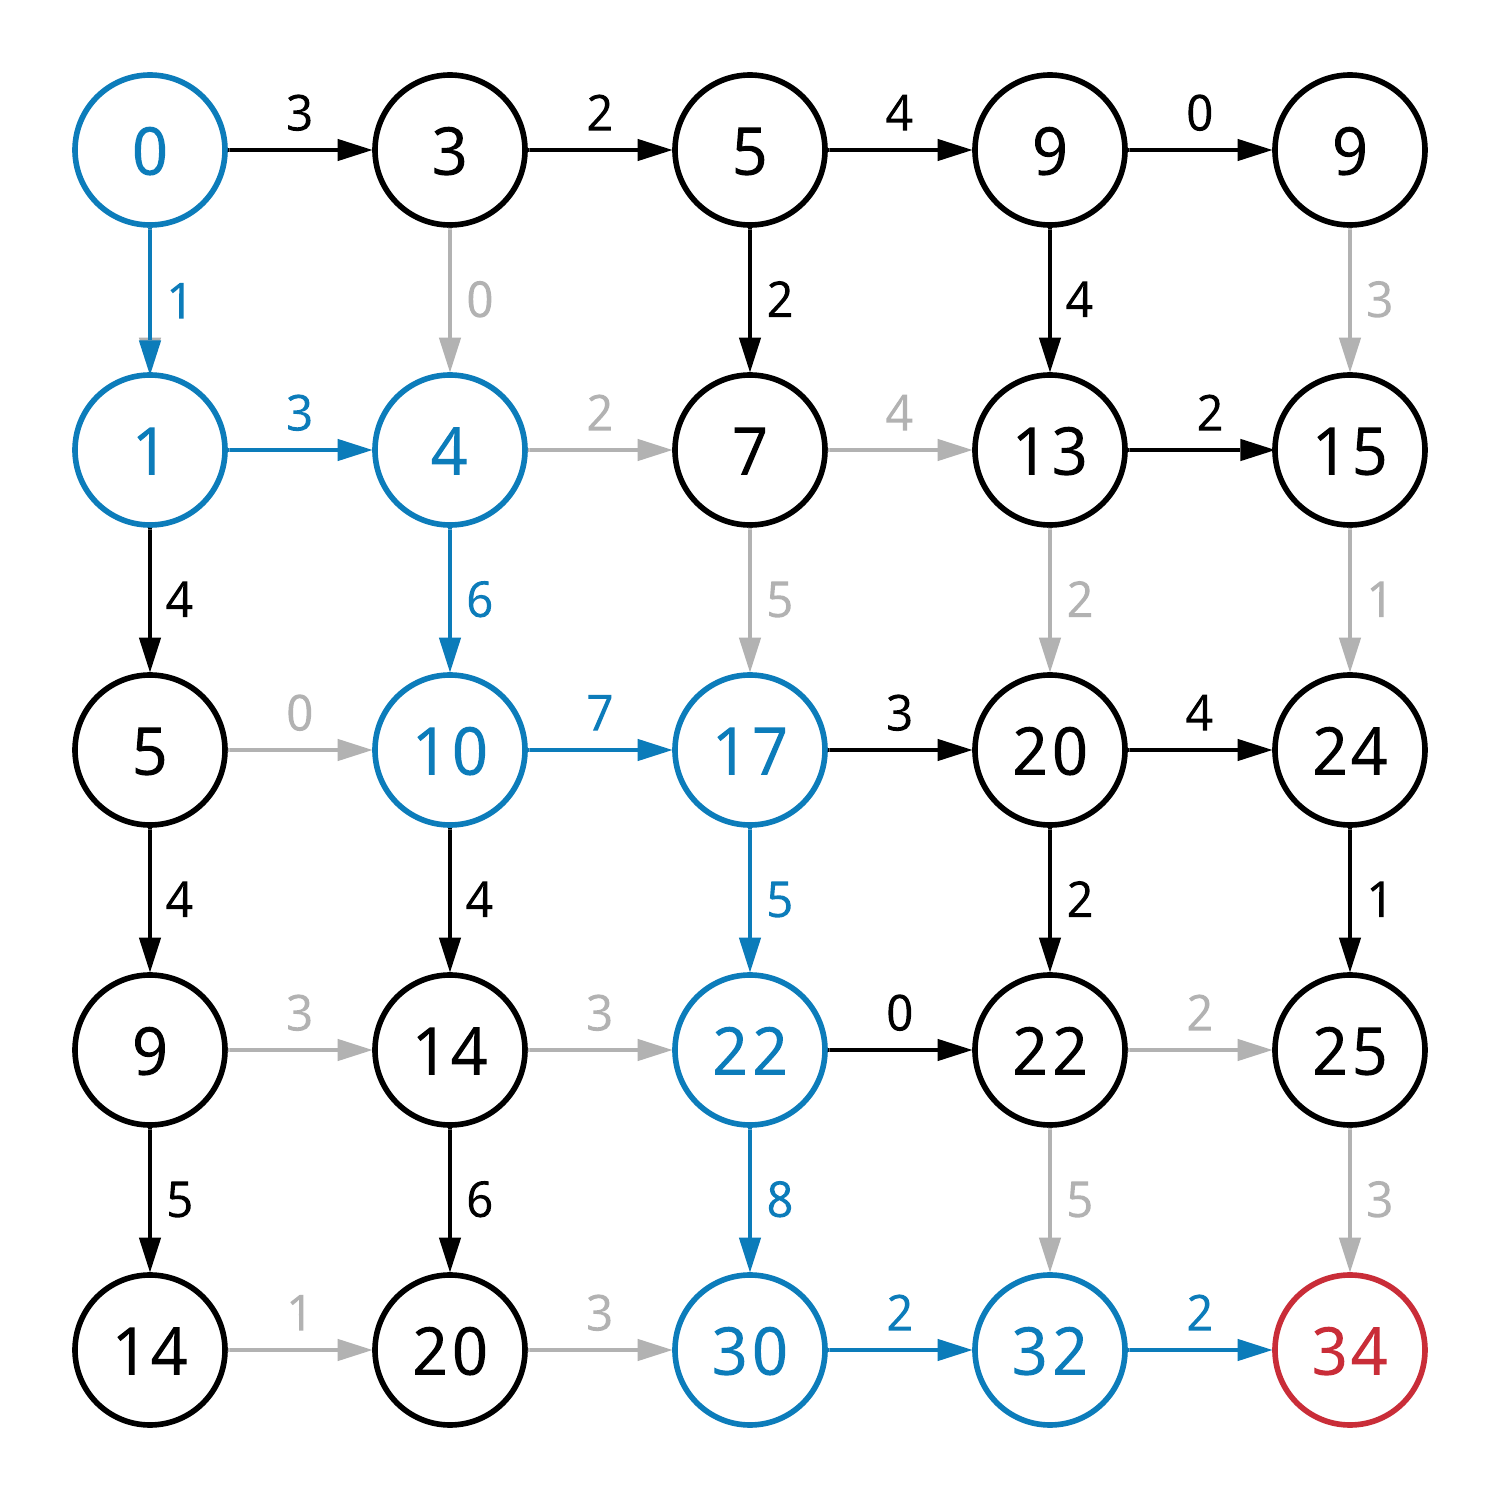
\includegraphics[scale=0.12]{c5/logos/5B.png}
\end{center}
\hline\vspace{5}

\subsection*{Formatting}
\noindent\textbf{Input:} Integers $n$ and $m$, followed by an $n\times(m+1)$ matrix \emph{Down}, and an $(n+1)\times m$ matrix \emph{Right}. The two matrices are separated by the "-" symbol.\\
\noindent\textbf{Output:} The length of a longest path from source ($0$,$0$) to sink ($n$,$m$) in the $n\times m$ rectangular grid whose edges are defined by the matrices \emph{Down} and \emph{Right} as an integer.

\subsection*{Constraints}
\begin{itemize}
    \item The values of $n$ and $m$ will be between $1$ and $10^2$.
\end{itemize}
\pagebreak

\subsection*{\href{https://github.com/rjeveloff/BA_problemregister/tree/main/test_cases/chapter_5/5B}{Test Cases \gitlogo}}
\stepcounter{subsubsection}\subsubsection*{Case \arabic{subsubsection}}
\hline \vspace{5}
\textbf{Description:} The sample dataset is not actually run on your code.\\ \\
\noindent \textbf{Input:}\\
\code{4 4\\1 0 2 4 3\\4 6 5 2 1\\4 4 5 2 1\\5 6 8 5 3\\-\\3 2 4 0\\3 2 4 2\\0 7 3 3\\3 3 0 2\\1 3 2 2}\\ \\
\noindent \textbf{Output:}\\
\code{34}

\stepcounter{subsubsection}\subsubsection*{Case \arabic{subsubsection}}
\hline \vspace{5}
\textbf{Description:} This dataset checks that your code considers the first column of \emph{Down} and the last row of \emph{Right}. If there is some off-by-one error (possibly due to $0$/$1$ indexing confusion) in updating the dynamic programming matrix it could be possible to miss these edges.\\ \\
\noindent \textbf{Input:}\\
\code{2 2\\20 0 0\\20 0 0\\-\\0 0\\0 0\\10 10}\\ \\
\noindent \textbf{Output:}\\
\code{60}
\pagebreak

\stepcounter{subsubsection}\subsubsection*{Case \arabic{subsubsection}}
\hline \vspace{5}
\textbf{Description:} This dataset checks that your code considers the last column of Down and the first row of Right. If there is some off-by-one error (possibly due to $0$/$1$ indexing confusion) in updating the dynamic programming matrix it could be possible to miss these edges. This dataset is very similar to test case $2$.\\ \\
\noindent \textbf{Input:}\\
\code{2 2\\0 0 20\\0 0 20\\-\\10 10\\0 0\\0 0}\\ \\
\noindent \textbf{Output:}\\
\code{60}

\stepcounter{subsubsection}\subsubsection*{Case \arabic{subsubsection}}
\hline \vspace{5}
\textbf{Description:} This dataset checks that you are not using some sort of greedy approach to solving this problem. If the movement with the highest weight is chosen at each step the first entry of \emph{Down} should be chosen. This will result in missing the higher total weight that just goes all the way right then down.\\ \\
\noindent \textbf{Input:}\\
\code{2 2\\20 0 0\\0 0 0\\-\\0 30\\0 0\\0 0}\\ \\
\noindent \textbf{Output:}\\
\code{30}
\pagebreak

\stepcounter{subsubsection}\subsubsection*{Case \arabic{subsubsection}}
\hline \vspace{5}
\textbf{Description:} This dataset checks that your code can correctly parse and use inputs in which $n$ and $m$ are not the same. In all previous test datasets $n$ and $m$ were the same. If your output doesn’t match the correct output make sure that your dynamic programming matrix has the dimensions ($n+1$)$\times$($m+1$). In previous datasets your code could get away with creating a dynamic programming matrix with dimensions ($n+1$)$\times$($n+1$) or ($m+1$)$\times$($m+1$), but implementations relying on those dimensions will fail this dataset.\\ \\
\noindent \textbf{Input:}\\
\code{5 3\\20 5 0 10\\0 5 10 0\\10 10 0 15\\0 20 20 25\\30 10 5 30\\-\\0 30 15\\10 20 10\\10 10 20\\20 25 30\\15 35 40\\15 10 25}\\ \\
\noindent \textbf{Output:}\\
\code{175}

\stepcounter{subsubsection}\subsubsection*{Case \arabic{subsubsection}}
\hline \vspace{5}
\textbf{Description:} This dataset checks that your code can correctly parse and use inputs in which $n$ and $m$ are not the same. This dataset is similar to test dataset $5$.\\ \\
\noindent \textbf{Input:}\\
\code{3 5\\0 5 10 0 10 10\\15 0 20 20 25 30\\10 5 30 15 0 20\\-\\0 30 15 10 20\\10 10 10 20 20\\25 30 15 35 40\\15 10 25 15 20}\\ \\
\noindent \textbf{Output:}\\
\code{180}
\pagebreak

\stepcounter{subsubsection}\subsubsection*{Case \arabic{subsubsection}}
\hline \vspace{5}
\textbf{Description:} A larger dataset of the same size as that provided by the randomized autograder. Check input/output folders for this dataset.\\ \\
\pagebreak

\subsection{Find a Longest Common Subsequence of Two Strings}
\hline\vspace{5}
\textbf{Longest Common Subsequence Problem}\\
\emph{Find a longest common subsequence of two strings}.\\ \\
\textbf{Input:} Two strings.\\
\textbf{Output:} A longest common subsequence of these strings.
\begin{center}
    
\includegraphics[scale=0.24]{c5/logos/5C.png}
\end{center}
\hline\vspace{5}

\subsection*{Formatting}
\noindent\textbf{Input:} Two newline-separated strings $v$ and $w$.\\
\noindent\textbf{Output:} A longest common subsequence of $v$ and $w$ as a string.

\subsection*{Constraints}
\begin{itemize}
    \item The lengths of $v$ and $w$ will be between $1$ and $10^3$.
    \item Both $v$ and $w$ will be DNA strings.
\end{itemize}
\pagebreak

\subsection*{\href{https://github.com/rjeveloff/BA_problemregister/tree/main/test_cases/chapter_5/5C}{Test Cases \gitlogo}}
\stepcounter{subsubsection}\subsubsection*{Case \arabic{subsubsection}}
\hline \vspace{5}
\textbf{Description:} The sample dataset is not actually run on your code.\\ \\
\noindent \textbf{Input:}\\
\code{GACT\\ATG}\\ \\
\noindent \textbf{Output:}\\
\code{AT}

\stepcounter{subsubsection}\subsubsection*{Case \arabic{subsubsection}}
\hline \vspace{5}
\textbf{Description:} This dataset checks that you code solves the longest common \emph{subsequence} problem instead of the related longest common \emph{substring} problem. The longest common \emph{substring} between \codebold{ACTG}\code{AG} and \code{G}\codebold{ACTG}\code{G} is \code{ACGT}, but the longest common \emph{subsequence} between \codebold{ACGT}\code{A}\codebold{G} and \code{G}\codebold{ACTGG} is \code{ACTGG}.\\ \\
\noindent \textbf{Input:}\\
\code{ACTGAG\\GACTGG}\\ \\
\noindent \textbf{Output:}\\
\code{ACTGG}

\stepcounter{subsubsection}\subsubsection*{Case \arabic{subsubsection}}
\hline \vspace{5}
\textbf{Description:} This simple dataset is used to check if your code correctly reconstructs the longest common subsequence from the backtracking matrix. Common errors include forgetting to reverse the reconstruction before returning (result: \code{CA}), terminating reconstruction too early (result: \code{C}), and starting reconstruction too late (result: \code{A}). \\ \\
\noindent \textbf{Input:}\\
\code{AC\\AC}\\ \\
\noindent \textbf{Output:}\\
\code{AC}
\pagebreak

\stepcounter{subsubsection}\subsubsection*{Case \arabic{subsubsection}}
\hline \vspace{5}
\textbf{Description:} This dataset checks that your code correctly considers the last character of each string. Off-by-one errors (can be caused by $0$/$1$ indexing errors) in indexing the input strings could result in the solution erroneously ignoring the final characters of inputs. If your code outputs an empty string it is likely that your implementation includes some off-by-one error.\\ \\
\noindent \textbf{Input:}\\
\code{GGGGT\\CCCCT}\\ \\
\noindent \textbf{Output:}\\
\code{T}

\stepcounter{subsubsection}\subsubsection*{Case \arabic{subsubsection}}
\hline \vspace{5}
\textbf{Description:} This dataset checks that your code correctly considers the first character of each string. Off-by-one errors (can be caused by $0$/$1$ indexing errors) in indexing the input strings could result in the solution erroneously ignoring the first characters of inputs. If your code outputs an empty string it is likely that your implementation includes some off-by-one error.\\ \\
\noindent \textbf{Input:}\\
\code{TCCCC\\TGGGG}\\ \\
\noindent \textbf{Output:}\\
\code{T}

\stepcounter{subsubsection}\subsubsection*{Case \arabic{subsubsection}}
\hline \vspace{5}
\textbf{Description:} This dataset checks that your code can handle inputs in which the two strings to be aligned are different lengths. If your output is incorrect make sure that your dynamic programming matrix has dimensions ($|v|+1$)$\times$($|w|+1$) or ($|w|+1$)$\times$($|v|+1$). If your code incorrectly sets the dynamic programming matrix dimensions to ($|v|+1$)$\times$($|v|+1$) or ($|w|+1$)$\times$($|w|+1$) it will not necessarily fail previous datasets since $|v|$ is the same as $|w|$ in all previous test datasets. Make sure that your implementation does not make any assumptions about the sizes of strings $v$ and $w$.\\ \\
\noindent \textbf{Input:}\\
\code{AA\\CGTGGAT}\\ \\
\noindent \textbf{Output:}\\
\code{A}
\pagebreak

\stepcounter{subsubsection}\subsubsection*{Case \arabic{subsubsection}}
\hline \vspace{5}
\textbf{Description:} This dataset checks that your code can handle inputs in which the two strings to be aligned are different lengths. This dataset is similar to test dataset $6$ except that in this dataset string $v$ is longer than string $w$.\\ \\
\noindent \textbf{Input:}\\
\code{GGTGACGT\\CT}\\ \\
\noindent \textbf{Output:}\\
\code{CT}

\stepcounter{subsubsection}\subsubsection*{Case \arabic{subsubsection}}
\hline \vspace{5}
\textbf{Description:} A larger dataset of the same size as that provided by the randomized autograder. Check input/output folders for this dataset.\\ \\
\pagebreak

\subsection{Find a Longest Path in a DAG}
\hline\vspace{5}
\textbf{Longest Path in a DAG Problem}\\
\emph{Find the longest path between two nodes in an edge-weighted DAG}.\\ \\
\textbf{Input:} An edge-weighted directed acyclic graph (DAG) and nodes \emph{Source} and \emph{Sink} in this DAG.\\
\textbf{Output:} A longest path from \emph{Source} to \emph{Sink} in this DAG and its length.
\begin{center}
    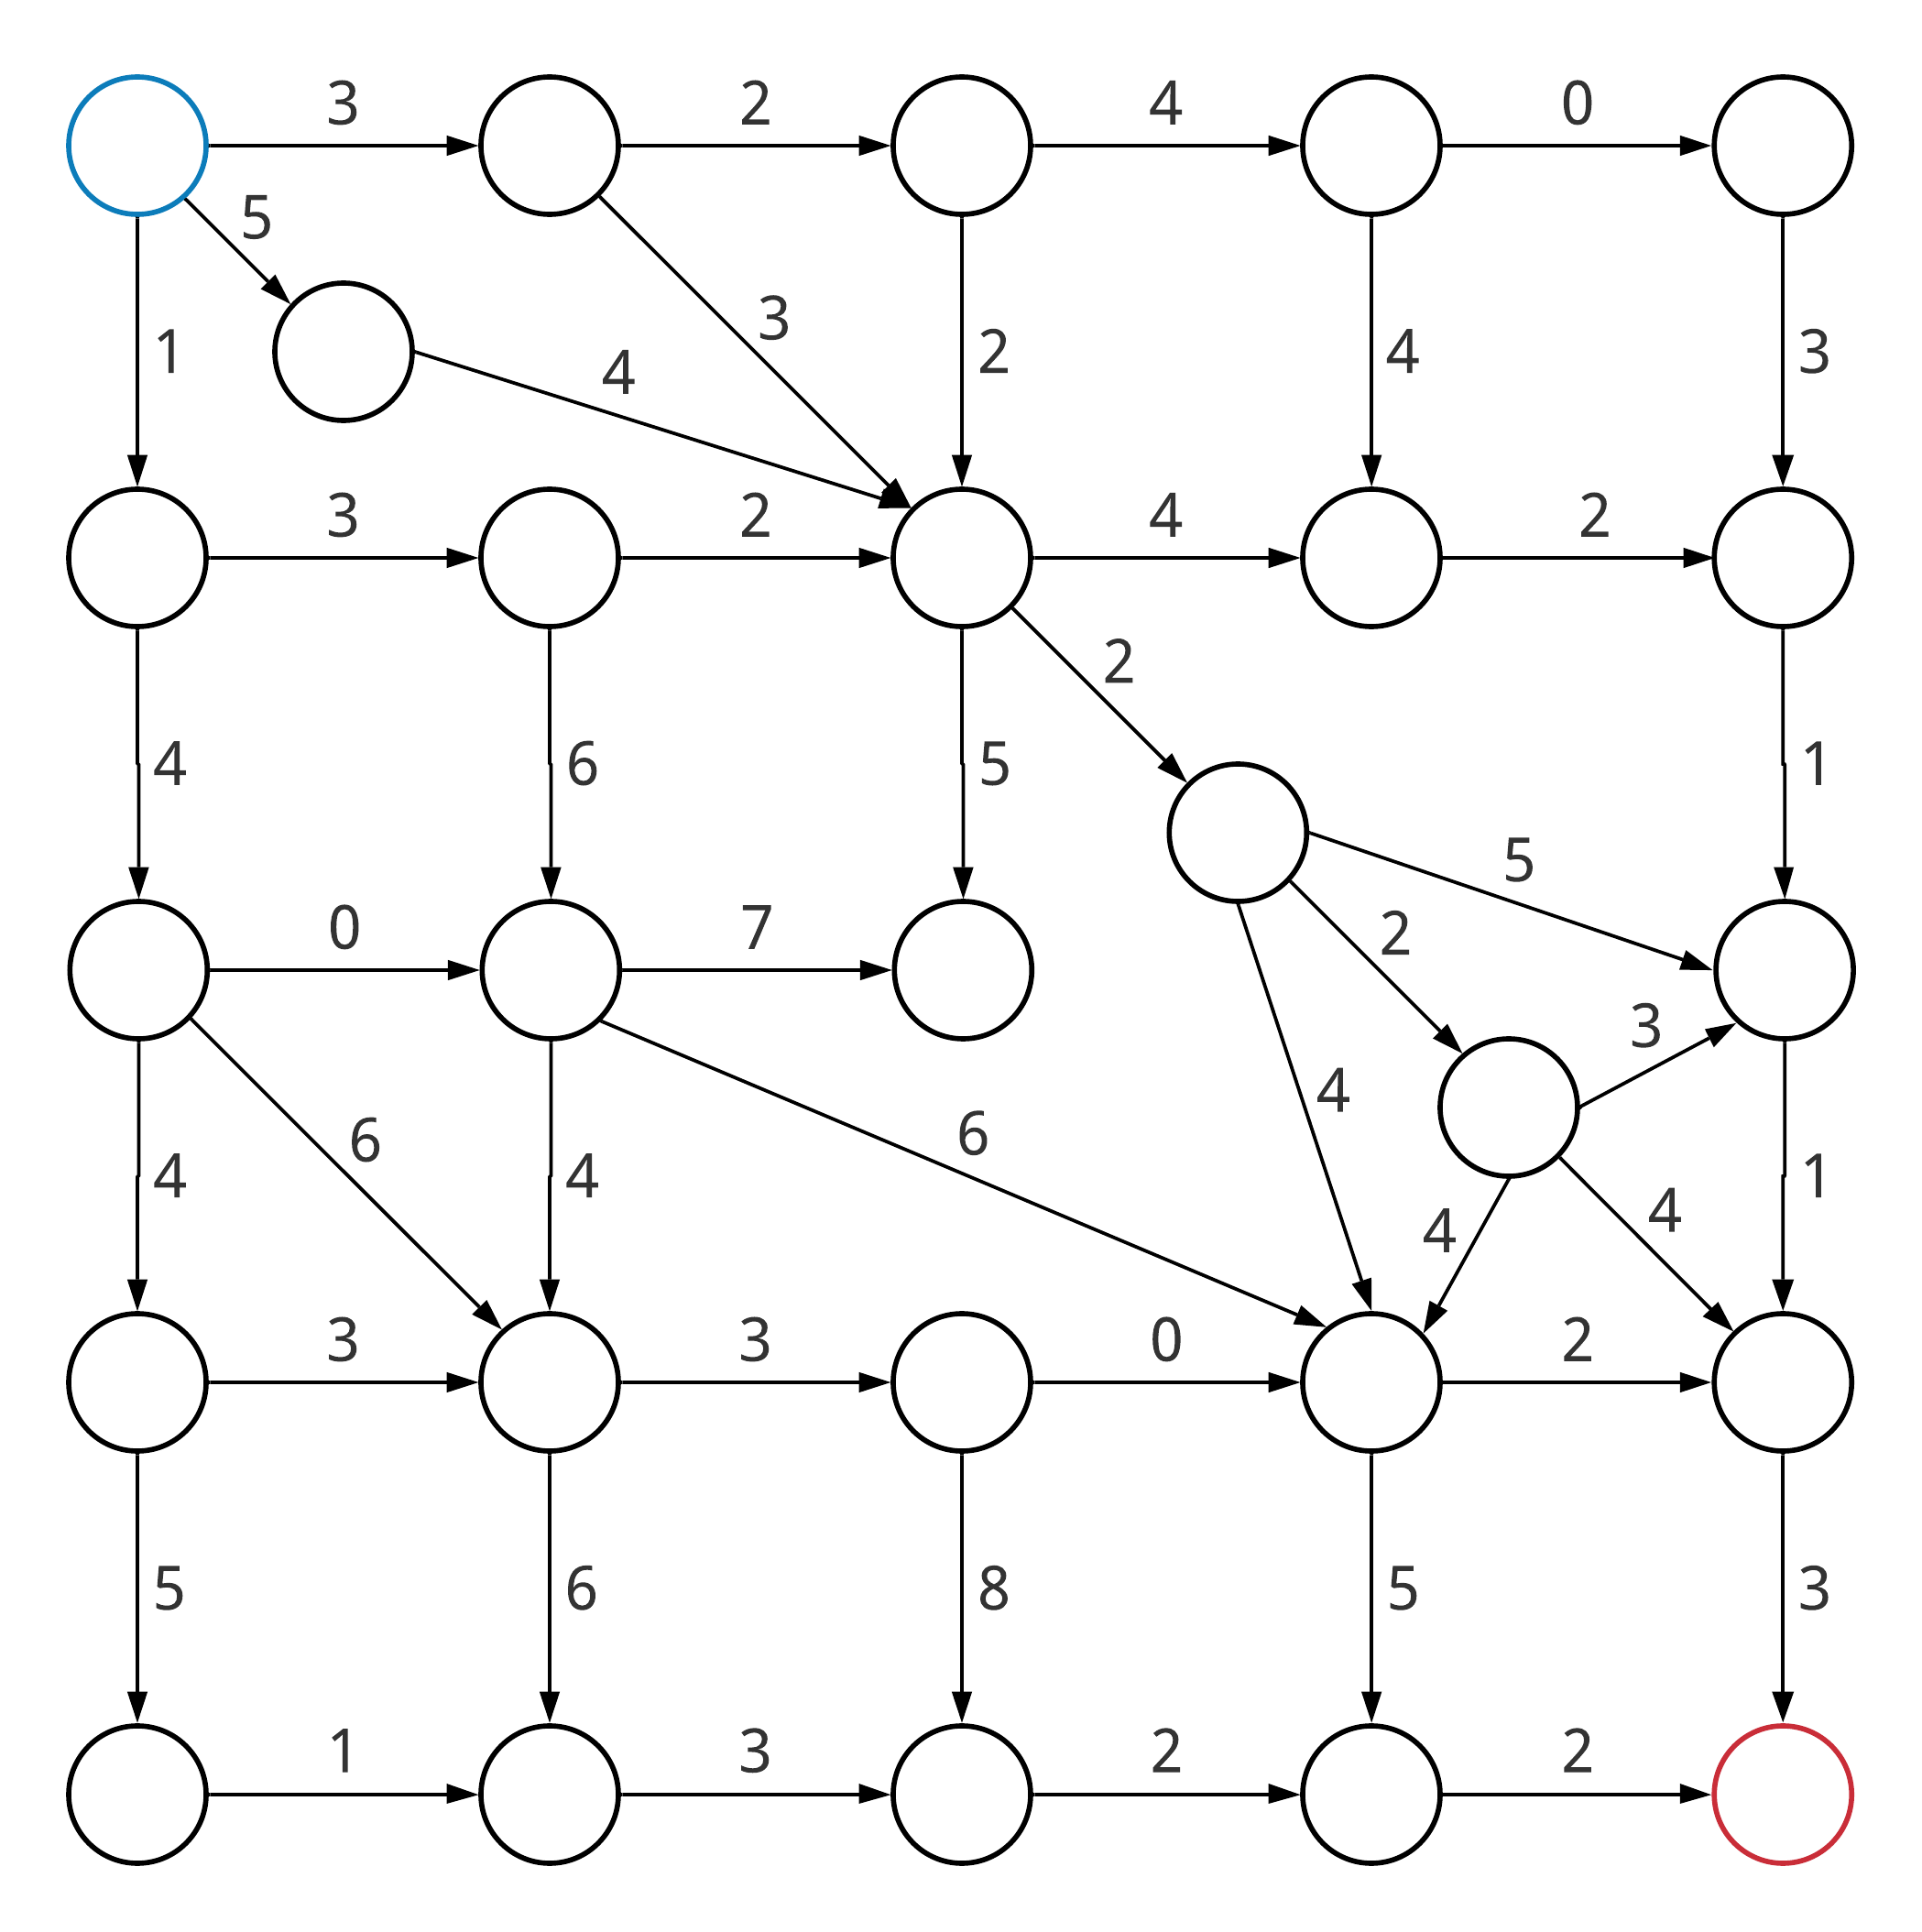
\includegraphics[scale=0.12]{c5/logos/5D.png}
\end{center}
\hline\vspace{5}

\subsection*{Formatting}
\noindent\textbf{Input:} Two space-separated integers labeling the source and sink nodes of an edge-weighted DAG, followed by an edge list representing an edge-weighted DAG.\\
\noindent\textbf{Output:} The length of a longest path in the edge-weighted DAG as an integer followed by a space-separated list of integers representing a longest path in the edge-weighted DAG (if multiple longest paths exist, you may return any one).

\subsection*{Constraints}
\begin{itemize}
    \item The values of \emph{Source} and \emph{Sink} will be between $1$ and $10^2$.
    \item The number of nodes in the DAG will be between $1$ and $10^2$.
    \item The number of edges in the DAG will be between $1$ and $10^2$.
    \item All nodes in the DAG will be labeled with integers.
    \item All edges in the DAG will have integer edge weights.
\end{itemize}
\pagebreak

\subsection*{\href{https://github.com/rjeveloff/BA_problemregister/tree/main/test_cases/chapter_5/5D}{Test Cases \gitlogo}}
\stepcounter{subsubsection}\subsubsection*{Case \arabic{subsubsection}}
\hline \vspace{5}
\textbf{Description:} The sample dataset is not actually run on your code.\\ \\
\noindent \textbf{Input:}\\
\code{0 4\\0 1 7\\0 2 4\\1 4 1\\2 3 2\\3 4 3}\\ \\
\noindent \textbf{Output:}\\
\code{9\\0 2 3 4}

\stepcounter{subsubsection}\subsubsection*{Case \arabic{subsubsection}}
\hline \vspace{5}
\textbf{Description:} This test makes sure that your code is actually finding the \emph{longest} path in a DAG not the \emph{shortest} path in a DAG. The \emph{shortest} path in this DAG goes $0$ $1$ $2$ $3$ with path length of $3$ while the \emph{longest} path goes $0$ $3$ with a path length of $10$. If your code outputs a path length of $3$ it is likely that you are finding the \emph{shortest} path instead of the \emph{longest} path.\\ \\
\noindent \textbf{Input:}\\
\code{0 3\\0 1 1\\0 3 10\\1 2 1\\2 3 1}\\ \\
\noindent \textbf{Output:}\\
\code{10\\0 3}
\pagebreak

\stepcounter{subsubsection}\subsubsection*{Case \arabic{subsubsection}}
\hline \vspace{5}
\textbf{Description:} This test makes sure that your code correctly parses the input. An input line of the form $x$ $y$ $z$ represents an edge from node $x$ to node $y$ with a weight of $z$. A common mistake is parsing the input so that $x$ $y$ $z$ represents an edge from node $x$ to node $z$ with weight $y$. If your code outputs a path length of $4$ with a path of $0$ $2$ $3$ it is likely that you are making the described parsing error.\\ \\
\noindent \textbf{Input:}\\
\code{0 3\\0 1 2\\0 2 1\\1 3 3\\2 3 3}\\ \\
\noindent \textbf{Output:}\\
\code{5\\0 1 3}

\stepcounter{subsubsection}\subsubsection*{Case \arabic{subsubsection}}
\hline \vspace{5}
\textbf{Description:} This test makes sure that your code isn’t an implementation of a greedy approach to this problem. A simple greedy approach that chooses paths at branching points based on edge weights at that point is not guaranteed return the correct output for this problem. If your code outputs a path weight of $6$ and a path of $0$ $2$ $3$ then it’s possible that you are using a greedy approach and fall into a non-optimal solution immediately by choosing the $0$ $2$ $5$ edge.\\ \\
\noindent \textbf{Input:}\\
\code{0 3\\0 1 1\\0 2 5\\1 3 10\\2 3 1}\\ \\
\noindent \textbf{Output:}\\
\code{11\\0 1 3}
\pagebreak

\stepcounter{subsubsection}\subsubsection*{Case \arabic{subsubsection}}
\hline \vspace{5}
\textbf{Description:} This test makes sure that your code does not rely on the source node being labeled $0$. This dataset is the same as test dataset $4$, except that each node label is incremented by one. If your output doesn’t match the correct output then your code likely assumes that the source node is labeled $0$. Make sure that your implementation uses the source node label from the input instead of making any assumptions about the label of the source node.\\ \\
\noindent \textbf{Input:}\\
\code{1 4\\1 2 1\\1 3 5\\2 4 10\\3 4 1}\\ \\
\noindent \textbf{Output:}\\
\code{11\\1 2 4}

\stepcounter{subsubsection}\subsubsection*{Case \arabic{subsubsection}}
\hline \vspace{5}
\textbf{Description:} This test makes sure that your code can correctly parse inputs in which there are double digit node labels. All previous datasets only have nodes with single digit labels, so if your code relies on node labels only having single digits it will likely fail on this dataset. If your output doesn’t match the correct output make sure that your code can handle nodes that have double digit labels.\\ \\
\noindent \textbf{Input:}\\
\code{1 10\\1 2 1\\2 3 3\\3 10 1}\\ \\
\noindent \textbf{Output:}\\
\code{5\\1 2 3 10}
\pagebreak

\stepcounter{subsubsection}\subsubsection*{Case \arabic{subsubsection}}
\hline \vspace{5}
\textbf{Description:} This test makes sure that your code can correctly handle inputs that only contain one edge. If your output doesn’t match the correct output make sure that your implementation doesn’t contain an off-by-one error that prevents the use of the only edge in the graph.\\ \\
\noindent \textbf{Input:}\\
\code{0 4\\0 4 7}\\ \\
\noindent \textbf{Output:}\\
\code{7\\0 4}

\stepcounter{subsubsection}\subsubsection*{Case \arabic{subsubsection}}
\hline \vspace{5}
\textbf{Description:} A larger dataset of the same size as that provided by the randomized autograder. Check input/output folders for this dataset.\\ \\
\pagebreak

\subsection{Find a Highest-Scoring Global Alignment of Two Strings}
\hline\vspace{5}
\textbf{Global Alignment Problem}\\
\emph{Find a highest-scoring global alignment between two strings using a scoring matrix}.\\ \\
\textbf{Input:} Two DNA strings, a match reward, a mismatch penalty, and an indel penalty.\\
\textbf{Output:} A highest-scoring global alignment of these two strings (with respect to the scoring matrix and the indel penalty) and its score.
\begin{center}
    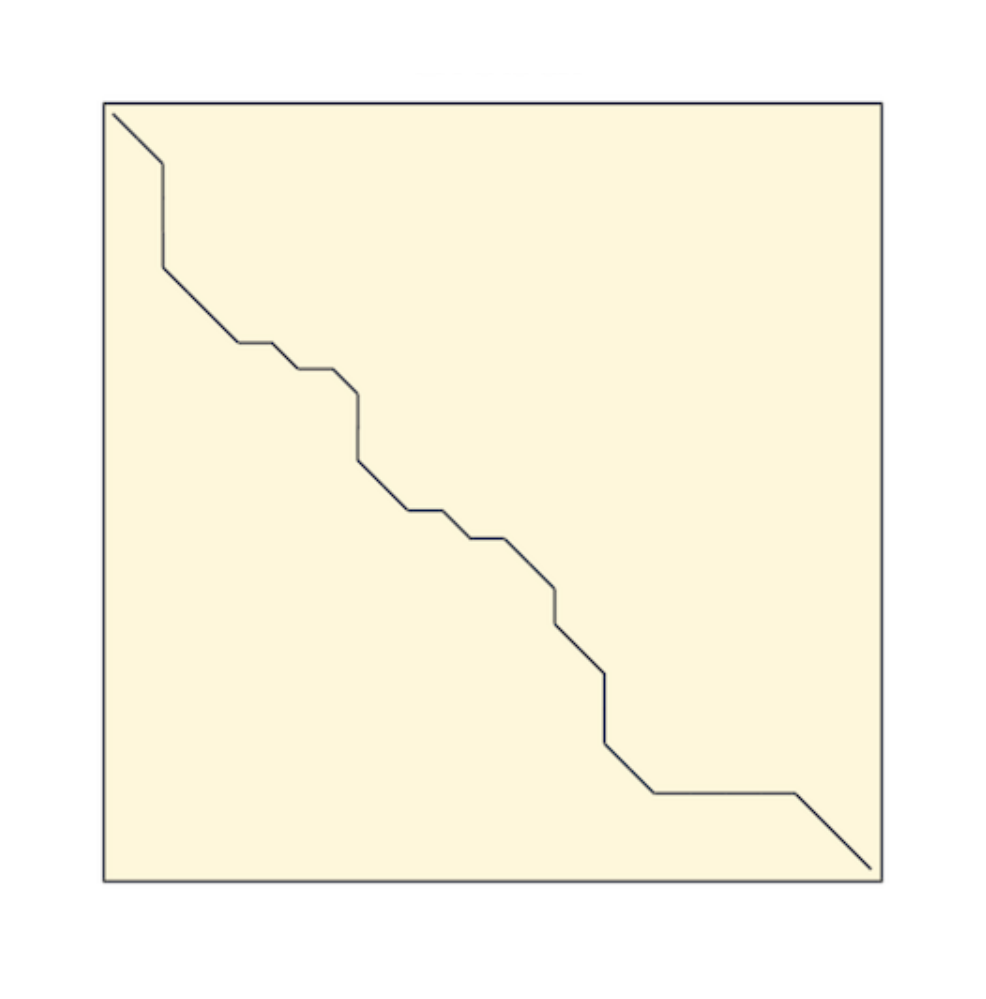
\includegraphics[scale=0.2]{c5/logos/5E.png}
\end{center}
\hline\vspace{5}

\subsection*{Formatting}
\noindent\textbf{Input:} Two space-separated DNA strings $v$ and $w$.\\
\noindent\textbf{Output:} The maximum global alignment score of $v$ and $w$ as an integer followed by a newline-separated global alignment of $v$ and $w$ achieving this maximum score (if multiple global alignments achieving the maximum score exist, you may return any one). Use a simple scoring function in which the match reward is equal to $1$, the mismatch penalty is equal to $1$, and the indel penalty is equal to $5$.

\subsection*{Constraints}
\begin{itemize}
    \item The lengths of $v$ and $w$ will be between $1$ and $10^4$.
    \item Both $v$ and $w$ will be DNA strings.
\end{itemize}
\pagebreak

\subsection*{\href{https://github.com/rjeveloff/BA_problemregister/tree/main/test_cases/chapter_5/5E}{Test Cases \gitlogo}}
\stepcounter{subsubsection}\subsubsection*{Case \arabic{subsubsection}}
\hline \vspace{5}
\textbf{Description:} The sample dataset is not actually run on your code.\\ \\
\noindent \textbf{Input:}\\
\code{1 1 2\\GAGA\\GAT}\\ \\
\noindent \textbf{Output:}\\
\code{-1\\GAGA\\GA-T}

\stepcounter{subsubsection}\subsubsection*{Case \arabic{subsubsection}}
\hline \vspace{5}
\textbf{Description:} This test makes sure that your code correctly parses the first line of input and uses the correct penalties. The mismatch $\mu$ and indel $\sigma$ penalties can easily be mistakenly swapped either when parsing the input or when actually applying the global alignment algorithm. In this case the mismatch penalty is more than twice the indel penalty. Therefore ending the alignment with two indels is better than simply aligning the mismatched final bases. If the mismatch and indel penalties were somehow switched in your code you will likely get a score of $1$ and an alignment of \code{ACG} and \code{ACT}.\\ \\
\noindent \textbf{Input:}\\
\code{1 3 1\\ACG\\ACT}\\ \\
\noindent \textbf{Output:}\\
\code{0\\AC-G\\ACT-}
\pagebreak

\stepcounter{subsubsection}\subsubsection*{Case \arabic{subsubsection}}
\hline \vspace{5}
\textbf{Description:} This test makes sure that the mismatch penalty is being correctly applied. A mismatch penalty of $1$ means that an alignment making use of mismatched bases suffer a score decrease of $1$. It can be easy to forget that penalties must be subtracted from the score, not added. Be sure that all penalties are being subtracted from score total when updating your dynamic programming matrix. Alternatively, you could negate the mismatch and indel penalties and add them to your scores. If your code outputs a score of $2$ or $3$ you are likely accidentally adding the penalties to your scores instead of subtracting them.\\ \\
\noindent \textbf{Input:}\\
\code{1 1 1\\AT\\AG}\\ \\
\noindent \textbf{Output:}\\
\code{0\\AT\\AG}

\stepcounter{subsubsection}\subsubsection*{Case \arabic{subsubsection}}
\hline \vspace{5}
\textbf{Description:} This test makes sure that your code allows for an output beginning with an indel. If your code doesn’t make use of the base cases (first row and column of the dynamic programming matrix) scores then the correct score of $3$ cannot be found. Be sure to correctly fill out your bases cases and consider them in your recursive cases.\\ \\
\noindent \textbf{Input:}\\
\code{2 5 1\\TCA\\CA}\\ \\
\noindent \textbf{Output:}\\
\code{3\\TCA\\-CA}
\pagebreak

\stepcounter{subsubsection}\subsubsection*{Case \arabic{subsubsection}}
\hline \vspace{5}
\textbf{Description:} This test makes sure that your code can handle multiple indels in a row. If there is some indel specific error in reconstructing the alignment from your backtracking matrix you may be missing an indel at the beginning or end of the second output string. This test also makes sure that the correct score calculation is being used for global alignment. This particular dataset would have a score of $2$ if fitting or local alignment were performed, but since this problem requires global alignment the preceding and trailing indels must be incorporated into the score.\\ \\
\noindent \textbf{Input:}\\
\code{1 10 1\\TTTTCCTT\\CC}\\ \\
\noindent \textbf{Output:}\\
\code{-4\\TTTTCCTT\\------CC---}

\stepcounter{subsubsection}\subsubsection*{Case \arabic{subsubsection}}
\hline \vspace{5}
\textbf{Description:} This test makes sure that your code can handles inputs in which the two strings differ drastically in length. Note that your reconstructed alignment may differ from the given output and is still correct as long as the "T" character in string $w$ is aligned to one of the "T" characters in string $v$. If your output doesn’t match the correct output make sure that your dynamic programming matrix has dimensions ($|v|+1$)$\times$($|w|+1$) or ($|w|+1$)$\times$($|v|+1$). If your code incorrectly set the dynamic programming matrix dimensions to ($|v|+1$)$\times$($|v|+1$) or ($|w|+1$)$\times$($|w|+1$) it will fail this case.\\ \\
\noindent \textbf{Input:}\\
\code{2 3 2\\ACAGATTAG\\T}\\ \\
\noindent \textbf{Output:}\\
\code{-14\\ACAGATTAG\\-------T-----}
\pagebreak

\stepcounter{subsubsection}\subsubsection*{Case \arabic{subsubsection}}
\hline \vspace{5}
\textbf{Description:} This test makes sure that your code can handles inputs in which the two strings differ drastically in length. This dataset is similar to test dataset $6$ except in this dataset string $v$ is much shorter than string $w$ instead of vice-versa.\\ \\
\noindent \textbf{Input:}\\
\code{3 1 2\\G\\ACATACGATG}\\ \\
\noindent \textbf{Output:}\\
\code{-15\\---------G------\\ACATACGATAG}

\stepcounter{subsubsection}\subsubsection*{Case \arabic{subsubsection}}
\hline \vspace{5}
\textbf{Description:} A larger dataset of the same size as that provided by the randomized autograder. Check input/output folders for this dataset.\\ \\
\pagebreak

\subsection{Find a Highest-Scoring Local Alignment of Two Strings}
\hline\vspace{5}
\textbf{Local Alignment Problem}\\
\emph{Find a highest-scoring local alignment between two strings}.\\ \\
\textbf{Input:} Two DNA strings, a match reward, a mismatch penalty, and an indel penalty.\\
\textbf{Output:} A highest-scoring local alignment of these two strings (with respect to the scoring matrix and the indel penalty) and its score.
\begin{center}
    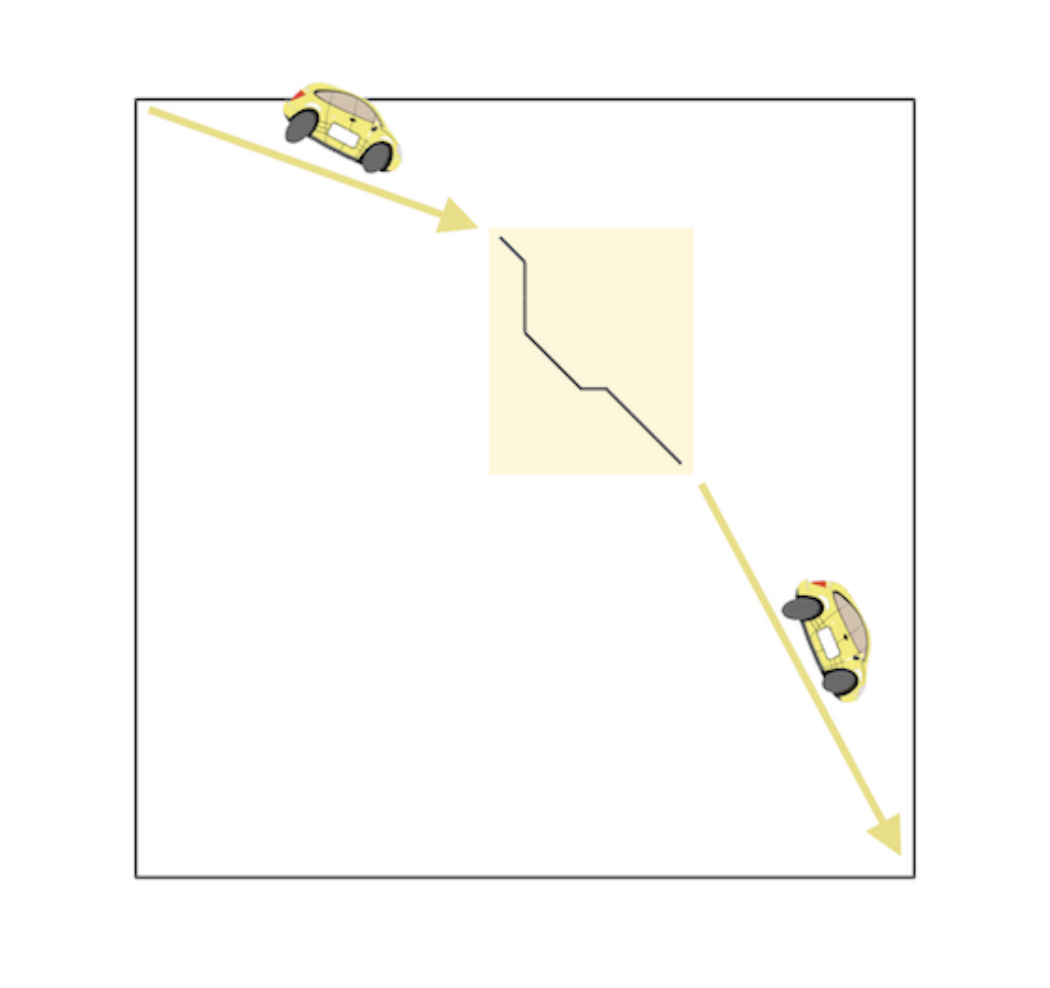
\includegraphics[scale=0.18]{c5/logos/5F.png}
\end{center}
\hline\vspace{5}

\subsection*{Formatting}
\noindent\textbf{Input:} Two space-separated DNA strings $v$ and $w$.\\
\noindent\textbf{Output:} The maximum local alignment score of $v$ and $w$ as an integer followed by a newline-separated local alignment of $v$ and $w$ achieving this maximum score (if multiple local alignments achieving the maximum score exist, you may return any one). Use a simple scoring function in which the match reward is equal to $1$, the mismatch penalty is equal to $1$, and the indel penalty is equal to $5$.

\subsection*{Constraints}
\begin{itemize}
    \item The lengths of $v$ and $w$ will be between $1$ and $10^4$.
    \item Both $v$ and $w$ will be DNA strings.
\end{itemize}
\pagebreak

\subsection*{\href{https://github.com/rjeveloff/BA_problemregister/tree/main/test_cases/chapter_5/5F}{Test Cases \gitlogo}}
\stepcounter{subsubsection}\subsubsection*{Case \arabic{subsubsection}}
\hline \vspace{5}
\textbf{Description:} The sample dataset is not actually run on your code.\\ \\
\noindent \textbf{Input:}\\
\code{1 1 2\\GAGA\\GAT}\\ \\
\noindent \textbf{Output:}\\
\code{2\\GA\\GA}

\stepcounter{subsubsection}\subsubsection*{Case \arabic{subsubsection}}
\hline \vspace{5}
\textbf{Description:} This test makes sure that your code correctly parses the first line of input and uses the correct penalties. The mismatch ($\mu$)and indel ($\sigma$) penalties can easily be mistakenly swapped either when parsing the input or when actually applying the local alignment algorithm. If the mismatch and indel penalties were somehow switched in your code you will likely get a score of $5$ and an alignment of \code{AGC} and \code{ATC}.\\ \\
\noindent \textbf{Input:}\\
\code{3 3 1\\AGC\\ATC}\\ \\
\noindent \textbf{Output:}\\
\code{4\\AG-C\\A-TC}
\pagebreak

\stepcounter{subsubsection}\subsubsection*{Case \arabic{subsubsection}}
\hline \vspace{5}
\textbf{Description:} This test makes sure that the mismatch penalties are being correctly applied. A mismatch penalty of $1$ means that an alignment making use of mismatched bases suffer a score \emph{decrease} of $1$. It can be easy to forget that penalties must be subtracted from the score, not added. Be sure that all penalties are being subtracted from score total when updating your dynamic programming matrix. Alternatively, you could negate the mismatch and indel penalties and add them to your scores. If your code outputs a score of $2$ or $3$ you are likely accidentally adding the penalties to your scores instead of subtracting them.\\ \\
\noindent \textbf{Input:}\\
\code{1 1 1\\AT\\AG}\\ \\
\noindent \textbf{Output:}\\
\code{1\\A\\A}

\stepcounter{subsubsection}\subsubsection*{Case \arabic{subsubsection}}
\hline \vspace{5}
\textbf{Description:} This test makes sure that your code can correctly find the highest scoring alignment, wherever it is in the dynamic programming matrix. This test also makes sure that your code correctly backtracks for local alignments. Be sure to terminate reconstruction of the aligned strings when a “free ride” can be used back to the origin. If your code doesn’t correctly terminate reconstruction it is possible that your score will be correct but your alignment will be incorrect.\\ \\
\noindent \textbf{Input:}\\
\code{1 1 1\\TAACG\\ACGTG}\\ \\
\noindent \textbf{Output:}\\
\code{3\\ACG\\ACG}
\pagebreak

\stepcounter{subsubsection}\subsubsection*{Case \arabic{subsubsection}}
\hline \vspace{5}
\textbf{Description:} This test makes sure that your code can handle inputs in which the strings vary drastically in length. If your output doesn’t match the correct output make sure that your implementation doesn’t make any assumptions about the lengths of the strings. Make sure that your dynamic programming matrix has dimensions ($|v|+1$)$\times$($|w|+1$) or ($|w|+1$)$\times$($|v|+1$). If your code incorrectly sets the dynamic programming matrix dimensions to ($|v|+1$)$\times$($|v|+1$) or ($|w|+1$)$\times$($|w|+1$) it will not necessarily fail previous datasets since $|v|$ is the same as $|w|$ in all previous test datasets but it will fail this one.\\ \\
\noindent \textbf{Input:}\\
\code{3 2 1\\CAGAGATGGCCG\\ACG}\\ \\
\noindent \textbf{Output:}\\
\code{6\\CG\\CG}

\stepcounter{subsubsection}\subsubsection*{Case \arabic{subsubsection}}
\hline \vspace{5}
\textbf{Description:} This dataset checks that your code can handle inputs in which the two strings to be aligned are different lengths. This dataset is similar to test dataset $5$ except that in this dataset string $v$ is shorter than string $w$.\\ \\
\noindent \textbf{Input:}\\
\code{2 3 1\\CTT\\AGCATAAAGCATT}\\ \\
\noindent \textbf{Output:}\\
\code{5\\C-TT\\CATT}

\stepcounter{subsubsection}\subsubsection*{Case \arabic{subsubsection}}
\hline \vspace{5}
\textbf{Description:} A larger dataset of the same size as that provided by the randomized autograder. Check input/output folders for this dataset.\\ \\
\pagebreak

\subsection{Compute the Edit Distance Between Two Strings}
\hline\vspace{5}
\textbf{Edit Distance Problem}\\
\emph{Find the edit distance between two strings}.\\ \\
\textbf{Input:} Two strings.\\
\textbf{Output:} The edit distance between these strings.
\begin{center}
    \includegraphics[scale=0.2]{c5/logos/5G.png}
\end{center}
\hline\vspace{5}

\subsection*{Formatting}
\noindent\textbf{Input:} Two space-separated strings $v$ and $w$.\\
\noindent\textbf{Output:} The edit distance between $v$ and $w$ as an integer.

\subsection*{Constraints}
\begin{itemize}
    \item The lengths of $v$ and $w$ will be between $1$ and $10^4$.
\end{itemize}
\pagebreak

\subsection*{\href{https://github.com/rjeveloff/BA_problemregister/tree/main/test_cases/chapter_5/5G}{Test Cases \gitlogo}}
\stepcounter{subsubsection}\subsubsection*{Case \arabic{subsubsection}}
\hline \vspace{5}
\textbf{Description:} The sample dataset is not actually run on your code.\\ \\
\noindent \textbf{Input:}\\
\code{GAGA\\GAT}\\ \\
\noindent \textbf{Output:}\\
\code{2}

\stepcounter{subsubsection}\subsubsection*{Case \arabic{subsubsection}}
\hline \vspace{5}
\textbf{Description:} This test makes sure that your code doesn’t reward exact matches by adding a positive value to the edit distance. If two strings are exactly the same then their edit distance should be $0$. It is easy to confuse edit distance with alignment, which could lead you to assign positive values to character matches in the dynamic programming matrix. When computing edit distance we only want to add to the edit distance when there is an indel or a mismatch. If your code outputs some multiple of $2$ for this dataset it is likely that there is some mistake regarding the nature of edit distance computation. Alternatively your code could be finding \emph{maximum} edit distance instead of \emph{minimum} edit distance. This is an especially easy mistake to make when coming from alignment problems.\\ \\
\noindent \textbf{Input:}\\
\code{AC\\AC}\\ \\
\noindent \textbf{Output:}\\
\code{0}
\pagebreak

\stepcounter{subsubsection}\subsubsection*{Case \arabic{subsubsection}}
\hline \vspace{5}
\textbf{Description:} This test makes sure that your code correctly adds to the edit distance between the two strings when there are deletions or substitutions. Any sort of edit operation will add $1$ to the edit distance between the two strings. If you are conflating alignment scores and edit distance it may be possible for you to come up with a negative result for this dataset. Don’t forget that all singular edit operations contribute exactly $1$ to the edit distance between strings; don’t add different values to the edit distance for insertions, deletions, and substitutions.\\ \\
\noindent \textbf{Input:}\\
\code{AT\\G}\\ \\
\noindent \textbf{Output:}\\
\code{2}

\stepcounter{subsubsection}\subsubsection*{Case \arabic{subsubsection}}
\hline \vspace{5}
\textbf{Description:} This test makes sure that your code correctly handles inputs in which the strings to be compared drastically differ in length. If your output doesn’t match the correct output make sure that your implementation makes no assumptions about the length of the strings to be compared. Make sure that your dynamic programming matrix has dimensions ($|v|+1$)$\times$($|w|+1$) or ($|w|+1$)$\times$($|v|+1$).\\ \\
\noindent \textbf{Input:}\\
\code{CAGACCGAGTTAG\\CGG}\\ \\
\noindent \textbf{Output:}\\
\code{10}

\stepcounter{subsubsection}\subsubsection*{Case \arabic{subsubsection}}
\hline \vspace{5}
\textbf{Description:} This test makes sure that your code correctly handles inputs in which the strings to be compared drastically differ in length. This test is similar to test dataset $4$ except in this dataset string $v$ is shorter than string $w$.\\ \\
\noindent \textbf{Input:}\\
\code{CGT\\CAGACGGTGACG}\\ \\
\noindent \textbf{Output:}\\
\code{9}
\pagebreak

\stepcounter{subsubsection}\subsubsection*{Case \arabic{subsubsection}}
\hline \vspace{5}
\textbf{Description:} A larger dataset of the same size as that provided by the randomized autograder. Check input/output folders for this dataset.\\ \\
\pagebreak

\subsection{Find a Highest-Scoring Fitting Alignment of Two Strings}
\hline\vspace{5}
\textbf{Fitting Alignment Problem}\\
\emph{Find a highest-scoring fitting alignment between two strings}.\\ \\
\textbf{Input:} Two amino acid strings, a $20\times 20$ scoring matrix, and an indel penalty.\\
\textbf{Output:} A highest-scoring fitting alignment of these two strings (with respect to the scoring matrix and the indel penalty) and its score.
\begin{center}
    \includegraphics[scale=0.2]{c5/logos/5H.png}
\end{center}
\hline\vspace{5}

\subsection*{Formatting}
\noindent\textbf{Input:} Two space-separated DNA strings $v$ and $w$.\\
\noindent\textbf{Output:} The maximum local alignment score of $v$ and $w$ as an integer followed by a newline-separated local alignment of $v$ and $w$ achieving this maximum score (if multiple fitting alignments achieving the maximum score exist, you may return any one). Use the BLOSUM62 scoring matrix and an indel penalty of $1$.

\subsection*{Constraints}
\begin{itemize}
    \item The lengths of $v$ will be between $1$ and $10^4$
    \item The length of $w$ will be between $1$ and $10^3$.
    \item Both $v$ and $w$ will be DNA strings.
\end{itemize}
\pagebreak

\subsection*{\href{https://github.com/rjeveloff/BA_problemregister/tree/main/test_cases/chapter_5/5H}{Test Cases \gitlogo}}
\stepcounter{subsubsection}\subsubsection*{Case \arabic{subsubsection}}
\hline \vspace{5}
\textbf{Description:} The sample dataset is not actually run on your code.\\ \\
\noindent \textbf{Input:}\\
\code{1 1 2\\GAGA\\GAT}\\ \\
\noindent \textbf{Output:}\\
\code{1\\GAG\\GAT}

\stepcounter{subsubsection}\subsubsection*{Case \arabic{subsubsection}}
\hline \vspace{5}
\textbf{Description:} This test makes sure that your dynamic programming matrix is correctly initialized. There should be no score punishment for starting at an arbitrary position in string $v$. Additionally, indels outside of string $w$ should not be reported in the final alignment. If your reconstructed alignment is the whole alignment below instead of the darkened portions then double check that your alignment reconstruction implementation does not include characters that do not fall within string $w$. If your code outputs a score of $0$ then make sure that the base cases in your dynamic programming matrix are correctly set.\\ \\
\noindent \textbf{Input:}\\
\code{1 1 1\\CCAT\\AT}\\ \\
\noindent \textbf{Output:}\\
\code{2\\AT\\AT}
\pagebreak

\stepcounter{subsubsection}\subsubsection*{Case \arabic{subsubsection}}
\hline \vspace{5}
\textbf{Description:} This test makes sure that your code isn’t mistakenly implementing local or global alignment instead of fitting alignment. If you are implementing local alignment you’ll get a score of $1$. If you are implementing global alignment you’ll get a score of $-2$. Be careful not to confuse the different types of alignment.\\ \\
\noindent \textbf{Input:}\\
\code{1 5 1\\CACGTC\\AT}\\ \\
\noindent \textbf{Output:}\\
\code{0\\ACGT\\A--T}

\stepcounter{subsubsection}\subsubsection*{Case \arabic{subsubsection}}
\hline \vspace{5}
\textbf{Description:} This test makes sure that your code chooses the correct cell in the dynamic programming matrix as the final score for the fitting alignment. If your implementation outputs the score in the bottom right corner of the matrix as it would be done in global alignment you will get a score of $0$. Also be sure that your code correctly backtracks from the final score cell and reconstructs the alignment.\\ \\
\noindent \textbf{Input:}\\
\code{1 1 1\\ATCC\\AT}\\ \\
\noindent \textbf{Output:}\\
\code{2\\AT\\AT}
\pagebreak

\stepcounter{subsubsection}\subsubsection*{Case \arabic{subsubsection}}
\hline \vspace{5}
\textbf{Description:} This test makes sure that your code can handle inputs in which the two strings are the same size. The constraints on this problem only state that $|w|\leq|v|$, so the length of the two strings are allowed to be equal. If your output doesn’t match the correct output make sure that your implementation doesn’t rely on the length of string $w$ being strictly less than the length of string $v$.\\ \\
\noindent \textbf{Input:}\\
\code{2 3 1\\ACGACAGAG\\CGAGAGGTT}\\ \\
\noindent \textbf{Output:}\\
\code{7\\CGACAGAG----\\CG---AGAGGTT}

\stepcounter{subsubsection}\subsubsection*{Case \arabic{subsubsection}}
\hline \vspace{5}
\textbf{Description:} This test makes sure that your code can correctly handles cases in which string $v$ is significantly longer than string $w$. In this dataset also has a high match score and low indel and mismatch penalties, incentivizing matching characters at any cost. If your output doesn’t match the correct output make sure that your implementation is correctly parsing the scoring scheme and not making any assumptions about the lengths of the strings to be aligned.\\ \\
\noindent \textbf{Input:}\\
\code{10 1 1\\CAAGACTACTATTAG\\GG}\\ \\
\noindent \textbf{Output:}\\
\code{10\\GACTACTATTAG\\G---------------G}

\stepcounter{subsubsection}\subsubsection*{Case \arabic{subsubsection}}
\hline \vspace{5}
\textbf{Description:} A larger dataset of the same size as that provided by the randomized autograder. Check input/output folders for this dataset.\\ \\
\pagebreak

\subsection{Find a Highest-Scoring Overlap Alignment of Two Strings}
\hline\vspace{5}
\textbf{Overlap Alignment Problem}\\
\emph{Find a highest-scoring overlap alignment between two strings}.\\ \\
\textbf{Input:} Two DNA strings, a match reward, a mismatch penalty, and an indel penalty.\\
\textbf{Output:} A highest-scoring overlap alignment of these two strings (with respect to the scoring matrix and the indel penalty) and its score.
\begin{center}
    \includegraphics[scale=0.2]{c5/logos/5I.png}
\end{center}
\hline\vspace{5}

\subsection*{Formatting}
\noindent\textbf{Input:} Two space-separated amino strings $v$ and $w$.\\
\noindent\textbf{Output:} The maximum overlap alignment score of $v$ and $w$ as an integer followed by a newline-separated overlap alignment of $v$ and $w$ achieving this maximum score (if multiple overlap alignments achieving the maximum score exist, you may return any one). Use a simple scoring function in which the match reward is equal to $1$ and both the mismatch and indel penalties are equal to $2$.

\subsection*{Constraints}
\begin{itemize}
    \item The lengths of $v$ and $w$ will be between $1$ and $10^3$
    \item Both $v$ and $w$ will be DNA strings.
\end{itemize}
\pagebreak

\subsection*{\href{https://github.com/rjeveloff/BA_problemregister/tree/main/test_cases/chapter_5/5I}{Test Cases \gitlogo}}
\stepcounter{subsubsection}\subsubsection*{Case \arabic{subsubsection}}
\hline \vspace{5}
\textbf{Description:} The sample dataset is not actually run on your code.\\ \\
\noindent \textbf{Input:}\\
\code{1 1 2\\GAGA\\GAT}\\ \\
\noindent \textbf{Output:}\\
\code{1\\GA\\GA}

\stepcounter{subsubsection}\subsubsection*{Case \arabic{subsubsection}}
\hline \vspace{5}
\textbf{Description:} This test makes sure that your dynamic programming matrix is correctly initialized. Skipping characters at the beginning of string $v$ should not be associated with a score penalty since the suffix of string $v$ is the only part of interest. In other words, we can prepend any number of gaps to string $w$ without a score penalty. For example we can write this alignment as \code{CCAT} and \code{--AT} and simply ignore the gap sequence prepended to string $w$ and the characters they align to in string $v$.\\ \\
\noindent \textbf{Input:}\\
\code{1 1 1\\CCAT\\AT}\\ \\
\noindent \textbf{Output:}\\
\code{2\\AT\\AT}
\pagebreak

\stepcounter{subsubsection}\subsubsection*{Case \arabic{subsubsection}}
\hline \vspace{5}
\textbf{Description:} This test makes sure that your dynamic programming matrix is correctly penalizing indels in string $v$. Gaps at the beginning of a suffix of string $v$ must be penalized. In this dataset the mismatch penalty is much higher than the indel penalty so that the ideal overlap alignment has a gap in the first character of the string $v$ suffix. If your code outputs a score of $3$ then it is likely that you’re mistakenly not punishing gaps at the beginning of the suffix. If your code outputs an alignment similar to \code{AT} and \code{AT} then it’s likely that your alignment reconstruction is incorrectly removing characters. While characters from the beginning of string $v$ can be freely removed this is not the case for string $w$. Since our alignment uses the "C" character from string $w$ we must also include the gap it aligns to in string $v$.\\ \\
\noindent \textbf{Input:}\\
\code{1 5 1\\GAT\\CAT}\\ \\
\noindent \textbf{Output:}\\
\code{1\\-AT\\CAT}

\stepcounter{subsubsection}\subsubsection*{Case \arabic{subsubsection}}
\hline \vspace{5}
\textbf{Description:} This test makes sure that your code correctly ignores characters at the end of string $w$ if that results in a better alignment score. In overlap alignment only the prefix of string $w$ must be aligned. Adding the "G" character to the alignment will only hurt the score, so it is not used in an ideal overlap alignment of this dataset. If your code includes the "G" character from string $w$ in its output then make sure that you are selecting your final score from the correct place in your dynamic programming matrix. Also check to make sure your alignment reconstruction does not add extra characters to the final alignment.\\ \\
\noindent \textbf{Input:}\\
\code{1 5 1\\ATCACT\\AT}\\ \\
\noindent \textbf{Output:}\\
\code{1\\ACT\\A-T}
\pagebreak

\stepcounter{subsubsection}\subsubsection*{Case \arabic{subsubsection}}
\hline \vspace{5}
\textbf{Description:} This test makes sure that your code correctly ignores characters at the end of string $w$ if that results in a better alignment score. In overlap alignment only the prefix of string $w$ must be aligned. Adding the "G" character to the alignment will only hurt the score, so it is not used in an ideal overlap alignment of this dataset. If your code includes the "G" character from string $w$ in its output then make sure that you are selecting your final score from the correct place in your dynamic programming matrix. Also check to make sure your alignment reconstruction does not add extra characters to the final alignment.\\ \\
\noindent \textbf{Input:}\\
\code{1 1 5\\ATCACT\\ATG}\\ \\
\noindent \textbf{Output:}\\
\code{0\\CT\\AT}

\stepcounter{subsubsection}\subsubsection*{Case \arabic{subsubsection}}
\hline \vspace{5}
\textbf{Description:} This test makes sure that your code can handle inputs in which the strings vary drastically in length. If your output doesn’t match the correct output make sure that your implementation doesn’t make any assumptions about the lengths of the strings. Make sure that your dynamic programming matrix has dimensions ($|v|+1$)$\times$($|w|+1$) or ($|w|+1$)$\times$($|v|+1$). If your code incorrectly set the dynamic programming matrix dimensions to ($|v|+1$)$\times$($|v|+1$) or ($|w|+1$)$\times$($|w|+1$) it will fail this dataset.\\ \\
\noindent \textbf{Input:}\\
\code{3 2 1\\CAGAGATGGCCG\\ACG}\\ \\
\noindent \textbf{Output:}\\
\code{5\\-CG\\ACG}
\pagebreak

\stepcounter{subsubsection}\subsubsection*{Case \arabic{subsubsection}}
\hline \vspace{5}
\textbf{Description:} This dataset checks that your code can handle inputs in which the two strings to be aligned are different lengths. This dataset is similar to test dataset $6$ except that in this dataset string $v$ is shorter than string $w$.\\ \\
\noindent \textbf{Input:}\\
\code{2 3 1\\CTT\\AGCATAAAGCATT}\\ \\
\noindent \textbf{Output:}\\
\code{0\\---CT-T\\AGC-AT}

\stepcounter{subsubsection}\subsubsection*{Case \arabic{subsubsection}}
\hline \vspace{5}
\textbf{Description:} A larger dataset of the same size as that provided by the randomized autograder. Check input/output folders for this dataset.\\ \\
\pagebreak

\subsection{Align Two Strings Using Affine Gap Penalties}
\hline\vspace{5}
\textbf{Alignment with Affine Gap Penalties Problem}\\
\emph{Find the highest-scoring alignment between two strings (with affine gap penalties)}.\\ \\
\textbf{Input:} Two amino acid strings, a match reward, a mismatch penalty, a gap opening penalty, and a gap extension penalty.\\
\textbf{Output:} A highest-scoring global alignment with affine gap penalties of these two strings (with respect to the scoring matrix and the gap opening and gap extension penalties) and its score.
\begin{center}
    \includegraphics[scale=0.16]{c5/logos/5J.png}
\end{center}
\hline\vspace{5}

\subsection*{Formatting}
\noindent\textbf{Input:} Two space-separated amino strings $v$ and $w$.\\
\noindent\textbf{Output:} The maximum global alignment score of $v$ and $w$ using affine gap penalties and an alignment of $v$ and $w$ achieving this maximum score (if multiple global alignments with affine gap penalties achieving the maximum score exist, you may return any one). Use the BLOSUM62 scoring matrix, a gap opening penalty of $11$, and a gap extension penalty of $1$.

\subsection*{Constraints}
\begin{itemize}
    \item The lengths of $v$ and $w$ will be between $1$ and $10^2$
    \item Both $v$ and $w$ will be amino acid strings.
\end{itemize}
\pagebreak

\subsection*{\href{https://github.com/rjeveloff/BA_problemregister/tree/main/test_cases/chapter_5/5J}{Test Cases \gitlogo}}
\stepcounter{subsubsection}\subsubsection*{Case \arabic{subsubsection}}
\hline \vspace{5}
\textbf{Description:} The sample dataset is not actually run on your code.\\ \\
\noindent \textbf{Input:}\\
\code{1 3 2 1\\GA\\GTTA}\\ \\
\noindent \textbf{Output:}\\
\code{-1\\G---A\\GTTA}

\stepcounter{subsubsection}\subsubsection*{Case \arabic{subsubsection}}
\hline \vspace{5}
\textbf{Description:} This test makes sure that your code is correctly parsing the gap opening and gap extension penalties. If your code swaps the values for the extension and opening penalties then your score will likely be $1$ instead of the correct value of $-1$. The reconstructed alignment should not change even if you mix up the gap opening and gap extension penalties.\\ \\
\noindent \textbf{Input:}\\
\code{1 5 3 1\\TTT\\TT}\\ \\
\noindent \textbf{Output:}\\
\code{-1\\TTT\\TT-}
\pagebreak

\stepcounter{subsubsection}\subsubsection*{Case \arabic{subsubsection}}
\hline \vspace{5}
\textbf{Description:} This test makes sure that your code is implementing global alignment with affine gap penalties instead of fitting, overlap, or local alignment with affine gap penalties. All other types of alignment will simply align the two "AT" substrings and report a score of $2$. Be sure that your implementation is of \emph{global} alignment.\\ \\
\noindent \textbf{Input:}\\
\code{1 5 5 1\\GAT\\AT}\\ \\
\noindent \textbf{Output:}\\
\code{-3\\GAT\\-AT}

\stepcounter{subsubsection}\subsubsection*{Case \arabic{subsubsection}}
\hline \vspace{5}
\textbf{Description:} This test makes sure that your \emph{upper} and \emph{lower} matrices are correctly initialized. Be especially careful about your initialization of the first row of the lower matrix and the first column of the upper matrix. Depending on your backtracking implementation it is possible that you will get the correct alignment reported despite having an incorrect score. This is likely due to an issue in your initialization of the \emph{upper} and \emph{lower} matrices. If you consistently get a score of $-2$ instead of the correct $-3$ it is possible that your code is incorrectly considering gaps that span across the two strings as one gap. This is not the case; there should be two gap opening penalties in the alignment for this dataset.\\ \\
\noindent \textbf{Input:}\\
\code{1 5 2 1\\CCAT\\GAT}\\ \\
\noindent \textbf{Output:}\\
\code{-3\\-CCAT\\G---AT}
\pagebreak

\stepcounter{subsubsection}\subsubsection*{Case \arabic{subsubsection}}
\hline \vspace{5}
\textbf{Description:} This test makes sure that your code can handle a gap extension penalty that isn’t equal to one. If your output doesn’t match the correct output it’s likely that your implementation relies on the gap extension penalty being equal to one. Since all previous datasets set the gap extension penalty to one your code could have passed all previous tests without properly using the input to set the gap extension penalty.\\ \\
\noindent \textbf{Input:}\\
\code{1 2 3 2\\CAGGT\\TAC}\\ \\
\noindent \textbf{Output:}\\
\code{-8\\CAGGT\\TAC---}

\stepcounter{subsubsection}\subsubsection*{Case \arabic{subsubsection}}
\hline \vspace{5}
\textbf{Description:} This test makes sure that your code can handle inputs in which the two strings are the same length. If your output doesn’t match the correct output make sure that your code doesn’t make any assumptions about the lengths of the input strings. Since no previous dataset contained two strings with the same length your implementation could have passed all previous tests without handling the case where the two strings are the same length.\\ \\
\noindent \textbf{Input:}\\
\code{2 3 3 2\\GTTCCAGGTA\\CAGTAGTCGT}\\ \\
\noindent \textbf{Output:}\\
\code{-8\\---GT---TCCAGGTA\\CAGTAGTC----GT-}
\pagebreak

\stepcounter{subsubsection}\subsubsection*{Case \arabic{subsubsection}}
\hline \vspace{5}
\textbf{Description:} This test makes sure that your code can handle inputs in which the strings vary drastically in length. If your output doesn’t match the correct output make sure that your implementation doesn’t make any assumptions about the lengths of the strings. Make sure that your three dynamic programming matrices are assigned the correct dimensions given the input strings.\\ \\
\noindent \textbf{Input:}\\
\code{1 3 1 1\\AGCTAGCCTAG\\GT}\\ \\
\noindent \textbf{Output:}\\
\code{-7\\AGCTAGCCTAG\\-G-T----------}

\stepcounter{subsubsection}\subsubsection*{Case \arabic{subsubsection}}
\hline \vspace{5}
\textbf{Description:} This dataset checks that your code can handle inputs in which the two strings to be aligned are different lengths. This dataset is similar to test dataset $7$ except that in this dataset string $v$ is shorter than string $w$.\\ \\
\noindent \textbf{Input:}\\
\code{2 1 2 1\\AA\\CAGTGTCAGTA}\\ \\
\noindent \textbf{Output:}\\
\code{-7\\----------A---A\\CAGTGTCAGTA}
\pagebreak

\stepcounter{subsubsection}\subsubsection*{Case \arabic{subsubsection}}
\hline \vspace{5}
\textbf{Description:} This dataset checks that your code is actually using three distinct matrices to reconstruct the alignment. It may be tempting to reconstruct the alignment using only the \emph{middle} matrix but that could lead to subtle errors. If the last "A" character in string $v$ was not present the ideal alignment would match the "T" characters. Once the last "A" character is added mismatching the "T" in string $w$ with the "G" in string $v$ yields a higher final score. If your implementation only uses one matrix then you are likely assuming that knowing if a gap is being initialized or extended is sufficient for scoring. Using only one matrix to backtrack is not sufficient for every case.\\ \\
\noindent \textbf{Input:}\\
\code{5 2 15 5\\ACGTA\\ACT}\\ \\
\noindent \textbf{Output:}\\
\code{-12\\ACGTA\\ACT---}

\stepcounter{subsubsection}\subsubsection*{Case \arabic{subsubsection}}
\hline \vspace{5}
\textbf{Description:} A larger dataset of the same size as that provided by the randomized autograder. Check input/output folders for this dataset.\\ \\
\pagebreak

\subsection{Find a Middle Edge in an Alignment Graph in Linear Space}
\hline\vspace{5}
\textbf{Middle Edge in Linear Space Problem}\\
\emph{Find the middle edge in an alignment graph in linear space}.\\ \\
\textbf{Input:} Two amino acid strings.\\
\textbf{Output:} A middle edge in the alignment graph of these two strings.
\begin{center}
    \includegraphics[scale=0.32]{c5/logos/5K.png}
\end{center}
\hline\vspace{5}

\subsection*{Formatting}
\noindent\textbf{Input:} Two space-separated amino strings $v$ and $w$.\\
\noindent\textbf{Output:} A newline-separated pair of nodes as space-separated $x$ and $y$ coordinate pairs, where the first node is connected to the second node through the middle edge. The optimal path is defined by the BLOSUM62 scoring matrix and a linear indel penalty $\sigma=5$.

\subsection*{Constraints}
\begin{itemize}
    \item The lengths of $v$ and $w$ will be between $1$ and $10^2$
    \item Both $v$ and $w$ will be amino acid strings.
\end{itemize}
\pagebreak

\subsection*{\href{https://github.com/rjeveloff/BA_problemregister/tree/main/test_cases/chapter_5/5K}{Test Cases \gitlogo}}
\stepcounter{subsubsection}\subsubsection*{Case \arabic{subsubsection}}
\hline \vspace{5}
\textbf{Description:} The sample dataset is not actually run on your code.\\ \\
\noindent \textbf{Input:}\\
\code{1 1 2\\GAGA\\GAT}\\ \\
\noindent \textbf{Output:}\\
\code{2 2\\2 3}

\stepcounter{subsubsection}\subsubsection*{Case \arabic{subsubsection}}
\hline \vspace{5}
\textbf{Description:} This test makes sure that your code can identify horizontal middle edges. In the sample dataset the middle edge is diagonal, but the high mismatch penalty in this dataset forces indels into the alignment. The middle node can be either ($0$, $2$) or ($1$, $2$) but either way the middle edge must be horizontal (($1$, $2$) and ($1$, $3$) is also a valid answer). If your middle node is incorrect make sure that you’re combining \emph{FromSource} and \emph{ToSink} correctly. If the middle node is correct but your middle edge is incorrect it’s likely that you’re making some indexing mistake in choosing the second node for the edge. If you’re reversing the strings to calculate \emph{ToSink} remember to compensate for that reversal when choosing the indices for the second node in the middle edge.\\ \\
\noindent \textbf{Input:}\\
\code{1 5 1\\TTTT\\CC}\\ \\
\noindent \textbf{Output:}\\
\code{0 2\\0 3}
\pagebreak

\stepcounter{subsubsection}\subsubsection*{Case \arabic{subsubsection}}
\hline \vspace{5}
\textbf{Description:} This test makes sure that your code can handle finding the middle edge when the first string has an odd length. The definition of the middle column is $\lfloor\frac{m}{2}\rfloor$ where $m$ is the length of the string along the horizontal axis. In this case it should be the second column, indexed by $1$. If your middle node isn’t ($0$, $1$) then check to make sure you’re actually using the correct middle column for a string of odd length.\\ \\
\noindent \textbf{Input:}\\
\code{1 1 2\\GAT\\AT}\\ \\
\noindent \textbf{Output:}\\
\code{0 1\\1 2}

\stepcounter{subsubsection}\subsubsection*{Case \arabic{subsubsection}}
\hline \vspace{5}
\textbf{Description:} This test makes sure that your code can identify vertical middle edges. In the sample dataset the middle edge is diagonal, but the structure of the strings in this dataset makes mismatches detrimental. There are two possible middle nodes for this dataset: ($2$, $2$) or ($3$, $2$). The middle edge starting at ($2$, $2$) is vertical while the middle edge starting at ($3$, $2$) is diagonal. If you want to make sure that your code can identify vertical middle edges choose the first maximum score in \emph{Length}. In this dataset, \emph{Length} should be [$-3$, $0$, $3$, $3$, $0$, $-3$]. If you choose the first $3$ as the location of the middle node you’ll have a vertical middle edge corresponding to the first possible answer. If you choose the second $3$ you will have a diagonal middle edge corresponding to the second possible answer. Both answers are correct but it may be valuable in your debugging to test if your code can identify vertical edges when they’re a possibility.\\ \\
\noindent \textbf{Input:}\\
\code{1 1 1\\TTTT\\TTCTT}\\ \\
\noindent \textbf{Output:}\\
\code{2 2\\3 2}
\pagebreak

\stepcounter{subsubsection}\subsubsection*{Case \arabic{subsubsection}}
\hline \vspace{5}
\textbf{Description:} This test makes sure that your code correctly identifies the middle edge when the maximum value in \emph{Length} is the last value. This means that the middle edge must be horizontal. Depending on how you’re keeping track of previous values for the \emph{ToSink} array it is easy to introduce bugs when the middle node falls on the first or last value in \emph{ToSink}. If your code correctly finds the middle node but has the incorrect middle edge (i.e. the second node in your output is incorrect) then you are likely making a mistake in checking the previous values for the \emph{ToSink} array. Double check to make sure your determination of previous values is valid for edge cases in the \emph{ToSink} array.\\ \\
\noindent \textbf{Input:}\\
\code{1 5 1\\GAACCC\\G}\\ \\
\noindent \textbf{Output:}\\
\code{1 3\\1 4}

\stepcounter{subsubsection}\subsubsection*{Case \arabic{subsubsection}}
\hline \vspace{5}
\textbf{Description:} This test makes sure that your code correctly handle inputs in which the match score is not equal to one. If your output doesn’t match the correct output make sure that your implementation doesn’t make any assumptions about the scoring scheme of the dataset. It is possible that your code passes all previous datasets and fails this one while assuming the match score is equal to one. Make sure that your implementation uses the match score given in the input instead of hard-coding any value for the match score. This requirement applies to the mismatch and indel penalties as well, but those elements of the scoring scheme have varied in previous datasets and would likely cause an earlier test failure. \\ \\
\noindent \textbf{Input:}\\
\code{2 3 1\\ACAGT\\CAT}\\ \\
\noindent \textbf{Output:}\\
\code{1 2\\2 3}
\pagebreak

\stepcounter{subsubsection}\subsubsection*{Case \arabic{subsubsection}}
\hline \vspace{5}
\textbf{Description:} This test makes sure that your code correctly handle inputs where the length of string $v$ is equal to one. This dataset is similar to test dataset $5$ except string $v$ is one character long instead of string $w$. There are multiple possible middle edges for this dataset. If your output doesn’t match one of the correct outputs make sure that your implementation explicitly considers a case in which string $v$ is only one character long. Double check that your middle column is equal to zero. Also make sure that your middle column being equal to zero doesn’t invalidate any part of your implementation. Note that ($1$, $0$) ($2$, $0$) and ($2$, $0$) ($3$, $1$) are also valid answers.\\ \\
\noindent \textbf{Input:}\\
\code{2 5 3\\T\\AATCCC}\\ \\
\noindent \textbf{Output:}\\
\code{0 0\\1 0}

\stepcounter{subsubsection}\subsubsection*{Case \arabic{subsubsection}}
\hline \vspace{5}
\textbf{Description:} A larger dataset of the same size as that provided by the randomized autograder. Check input/output folders for this dataset.\\ \\
\pagebreak

\subsection{Align Two Strings Using Linear Space}
\hline\vspace{5}
\textbf{Global Alignment in Linear Space Problem}\\
\emph{Find a highest-scoring global alignment between two strings using a scoring matrix in linear space}.\\ \\
\textbf{Input:} Two amino acid strings, a $20\times 20$ scoring matrix, and an indel penalty.\\
\textbf{Output:} A highest-scoring global alignment of these two strings using linear space (with respect to the scoring matrix and the indel penalty) and its score.
\begin{center}
    \includegraphics[scale=0.32]{c5/logos/5L.png}
\end{center}
\hline\vspace{5}

\subsection*{Formatting}
\noindent\textbf{Input:} Two space-separated amino acid strings $v$ and $w$.\\
\noindent\textbf{Output:} The maximum global alignment score of $v$ and $w$ as an integer followed by a newline-separated global alignment of $v$ and $w$ achieving this maximum score (if multiple global alignments achieving the maximum score exist, you may return any one). Use the BLOSUM62 scoring matrix and an indel penalty $\sigma=5$.

\subsection*{Constraints}
\begin{itemize}
    \item The lengths of $v$ and $w$ will be between $1$ and $10^5$.
    \item Both $v$ and $w$ will be amino acid strings.
\end{itemize}
\pagebreak

\subsection*{\href{https://github.com/rjeveloff/BA_problemregister/tree/main/test_cases/chapter_5/5L}{Test Cases \gitlogo}}
\stepcounter{subsubsection}\subsubsection*{Case \arabic{subsubsection}}
\hline \vspace{5}
\textbf{Description:} The sample dataset is not actually run on your code.\\ \\
\noindent \textbf{Input:}\\
\code{1 1 2\\GAGA\\GAT}\\ \\
\noindent \textbf{Output:}\\
\code{-1\\GAGA\\GA-T}

\stepcounter{subsubsection}\subsubsection*{Case \arabic{subsubsection}}
\hline \vspace{5}
\textbf{Description:} The majority of bugs for this problem will likely be due to some uncaught mistake in the implementation of the Finding a Middle Edge in Alignment Graph in Linear Space Problem. Be sure that your middle edge implementation passes all given tests before working on this problem. This test makes sure that your code can handle runs of indels in the reconstructed alignment. If your score is incorrect be sure to check to make sure you are assigning the correct score to the middle edge. The error may stem from misidentification of the type of middle edge (match, mismatch, or indel) or from an indexing error when comparing the characters of the two strings to distinguish between matches and mismatches. If your output contains any mismatches there is probably some error in your reconstruction of the alignment.\\ \\
\noindent \textbf{Input:}\\
\code{1 5 1\\TT\\CC}\\ \\
\noindent \textbf{Output:}\\
\code{-4\\---TT\\CC---}
\pagebreak

\stepcounter{subsubsection}\subsubsection*{Case \arabic{subsubsection}}
\hline \vspace{5}
\textbf{Description:} This test makes sure that your code correctly mismatches characters when the ideal alignment requires it. In test dataset $1$, your code was tested for its ability to assign continuous indels when necessary; this dataset tests if your code is able to assign continuous mismatches if necessary. If there are any indels in your alignment and your score is correct, double check that your reconstruction methods are correct. If your score is incorrect check that your base cases correct update the score. Pay especial attention to the base cases of the recursive algorithm in both the score updating and alignment reconstruction steps. \\ \\
\noindent \textbf{Input:}\\
\code{1 1 5\\TT\\CC}\\ \\
\noindent \textbf{Output:}\\
\code{-2\\TT\\CC}

\stepcounter{subsubsection}\subsubsection*{Case \arabic{subsubsection}}
\hline \vspace{5}
\textbf{Description:} This test makes sure that your code correctly aligns the upper and lower sub-matrices after recursive calls. Be very careful to check that your \emph{top}, \emph{bottom}, \emph{left}, and \emph{right} values are correct for each recursive call since it’s very easy to have an off-by-one error that will become very difficult to debug on large datasets. To help debug any errors you may have on this dataset a trace of \emph{top}, \emph{bottom}, \emph{left}, and \emph{right} values is provided below. Your code does not necessarily need to have the exact same values as below (if there are ties in \emph{Length} scores).\\ \\
\noindent \textbf{Input:}\\
\code{1 5 1\\GAACGATTG\\GGG}\\ \\
\noindent \textbf{Output:}\\
\code{-3\\GAACGATTG\\G-----G-----G}
\pagebreak

\stepcounter{subsubsection}\subsubsection*{Case \arabic{subsubsection}}
\hline \vspace{5}
\textbf{Description:} This test makes sure that your code correctly handles inputs in which the match score is not equal to one. If your output doesn’t match the correct output make sure that your implementation doesn’t make any assumptions about the scoring scheme of the dataset. It is possible that your code passes all previous datasets and fails this one while assuming the match score is equal to one. Make sure that your implementation uses the match score given in the input instead of hard-coding any value for the match score. This requirement applies to the mismatch and indel penalties as well, but those elements of the scoring scheme have varied in previous datasets and would likely cause an earlier test failure.\\ \\
\noindent \textbf{Input:}\\
\code{2 3 1\\GCG\\CT}\\ \\
\noindent \textbf{Output:}\\
\code{-1\\GCG-\\-C-T}

\stepcounter{subsubsection}\subsubsection*{Case \arabic{subsubsection}}
\hline \vspace{5}
\textbf{Description:} This test makes sure that your code correctly handles inputs in which string $w$ is one character long. The correctness of your output for this dataset is largely reliant on the correctness of your underlying middle edge implementation. If your output doesn’t match the correct output make sure that your implementation of the middle edge algorithm passes test dataset $5$ in the Finding a Middle Edge in Alignment Graph in Linear Space Problem. That test also considers the case where string $w$ is one character long.\\ \\
\noindent \textbf{Input:}\\
\code{1 2 3\\ACAGCTA\\G}\\ \\
\noindent \textbf{Output:}\\
\code{-17\\ACAGCTA\\-----G-----}
\pagebreak

\stepcounter{subsubsection}\subsubsection*{Case \arabic{subsubsection}}
\hline \vspace{5}
\textbf{Description:} This test makes sure that your code correctly handles inputs in which string $v$ is one character long. The correctness of your output for this dataset is largely reliant on the correctness of your underlying middle edge implementation. If your output doesn’t match the correct output make sure that your implementation of the middle edge algorithm passes test dataset $6$ in the Finding a Middle Edge in Alignment Graph in Linear Space Problem. That test also considers the case where string $v$ is one character long.\\ \\
\noindent \textbf{Input:}\\
\code{3 4 1\\A\\CGGAGTGCC}\\ \\
\noindent \textbf{Output:}\\
\code{-5\\-----A--------\\CGGAGTGCC}

\stepcounter{subsubsection}\subsubsection*{Case \arabic{subsubsection}}
\hline \vspace{5}
\textbf{Description:} A larger dataset of the same size as that provided by the randomized autograder. Check input/output folders for this dataset.\\ \\
\pagebreak

\subsection{Find a Highest-Scoring Multiple Sequence Alignment}
\hline\vspace{5}
\textbf{Multiple Sequence Alignment Problem}\\
\emph{Find a highest-scoring alignment of multiple sequences}.\\ \\
\textbf{Input:} Three DNA strings and a simple scoring function.\\
\textbf{Output:} A highest-scoring multiple alignment of these strings (with respect to the scoring matrix and indel penalty) and its score.
\begin{center}
    \includegraphics[scale=0.24]{c5/logos/5M.png}
\end{center}
\hline\vspace{5}

\subsection*{Formatting}
\noindent\textbf{Input:} Three space-separated DNA strings $x$, $y$, and $z$.\\
\noindent\textbf{Output:} The maximum multiple sequence alignment score of $x$, $y$, and $z$ as an integer followed by a newline-separated multiple sequence alignment of $x$, $y$, and $z$ achieving this maximum score (if more than one multiple sequence alignments achieving the maximum score exist, you may return any one). Use a simple scoring function in which the score is equal to $1$.

\subsection*{Constraints}
\begin{itemize}
    \item The lengths of $x$, $y$, and $z$ will be between $1$ and $10^3$.
    \item Strings $x$, $y$, and $z$ will be DNA strings.
\end{itemize}
\pagebreak

\subsection*{\href{https://github.com/rjeveloff/BA_problemregister/tree/main/test_cases/chapter_5/5M}{Test Cases \gitlogo}}
\stepcounter{subsubsection}\subsubsection*{Case \arabic{subsubsection}}
\hline \vspace{5}
\textbf{Description:} The sample dataset is not actually run on your code.\\ \\
\noindent \textbf{Input:}\\
\code{ATATCGG\\TCCGA\\ATGTACTG}\\ \\
\noindent \textbf{Output:}\\
\code{3\\ATATCC-G-\\-----TCC-GA\\ATGTACTG-}

\stepcounter{subsubsection}\subsubsection*{Case \arabic{subsubsection}}
\hline \vspace{5}
\textbf{Description:} This test makes sure that your code follows the scoring scheme of the problem. The score will only increase if there is a match between all three strings. Otherwise the score remains unchanged. In this dataset your code should not penalize the indels in reconstructed alignment for strings $x$ and $z$.\\ \\
\noindent \textbf{Input:}\\
\code{A\\AT\\A}\\ \\
\noindent \textbf{Output:}\\
\code{1\\A-\\AT\\A-}
\pagebreak

\stepcounter{subsubsection}\subsubsection*{Case \arabic{subsubsection}}
\hline \vspace{5}
\textbf{Description:} This test makes sure that your code can accurately reconstruct the alignment when one of the aligned strings is primarily indels. When backtracking to reconstruct the alignment in this problem be sure to handle all the base cases. In regular two-string alignment you only need to worry about backtracking base cases for the very first row and the very first column of the dynamic programming matrix. In three-string alignment you also need to consider the two dimensional matrices formed by every possible pair of strings. These two dimensional matrices also need to be considered when backtracking.\\ \\
\noindent \textbf{Input:}\\
\code{AAAAT\\CCCCT\\T}\\ \\
\noindent \textbf{Output:}\\
\code{1\\AAAAT\\CCCCT\\------T}

\stepcounter{subsubsection}\subsubsection*{Case \arabic{subsubsection}}
\hline \vspace{5}
\textbf{Description:} This test makes sure that your code correctly forces a three character match whenever possible. The reconstructed alignment is not set in stone, just make sure that the first character and last character of the three strings align with each other. Note that in the example output extra indels are introduced when not necessary (mismatching "CC" and "GG" doesn’t have a penalty); the scoring scheme in this problem allows such an alignment. Make sure that your code does not unnecessarily punish extra indels.\\ \\
\noindent \textbf{Input:}\\
\code{AT\\ACCT\\AGGGGT}\\ \\
\noindent \textbf{Output:}\\
\code{2\\A---------T\\A------CCT\\AGGGG---T}
\pagebreak

\stepcounter{subsubsection}\subsubsection*{Case \arabic{subsubsection}}
\hline \vspace{5}
\textbf{Description:} This test makes sure that your code is able to output a score of zero if there are no matching characters between the three strings. For this dataset any alignment reconstruction that includes all characters from each string is acceptable. No matter how the three strings in this dataset are aligned there is no way to obtain a non-zero score. If your output score doesn’t match the correct output score make sure that your implementation doesn’t disallow a score of zero when necessary.\\ \\
\noindent \textbf{Input:}\\
\code{GGAG\\TT\\CCCC}\\ \\
\noindent \textbf{Output:}\\
\code{0\\------GGAG\\---TT------\\CCCC------}

\stepcounter{subsubsection}\subsubsection*{Case \arabic{subsubsection}}
\hline \vspace{5}
\textbf{Description:} This test makes sure that your code is able to correctly handle inputs in which all three strings are one character long. Since all the strings are the same in this dataset the output will have a score of one and the reconstructed alignment will be the same as the input. If your output doesn’t match the correct output it’s likely that your implementation has an error in reconstruction. If your code outputs extraneous gap characters in the reconstructed alignment there is likely an error in the termination of your reconstruction. Double check your base cases.\\ \\
\noindent \textbf{Input:}\\
\code{T\\T\\T}\\ \\
\noindent \textbf{Output:}\\
\code{1\\T\\T\\T}

\stepcounter{subsubsection}\subsubsection*{Case \arabic{subsubsection}}
\hline \vspace{5}
\textbf{Description:} A larger dataset of the same size as that provided by the randomized autograder. Check input/output folders for this dataset.\\ \\
\pagebreak

\subsection{Find a Topological Ordering of a DAG}
\hline\vspace{5}
\textbf{Topological Ordering Problem}\\
\emph{Find a topological ordering of a directed acyclic graph}.\\ \\
\textbf{Input:} A directed acyclic graph.\\
\textbf{Output:} A topological ordering of this graph.
\begin{center}
    \includegraphics[scale=0.2]{c5/logos/5N.png}
\end{center}
\hline\vspace{5}

\subsection*{Formatting}
\noindent\textbf{Input:} An adjacency list representing a directed acyclic graph with nodes represented by integers.\\
\noindent\textbf{Output:} A space-separated list of integers representing a topological ordering of the DAG.

\subsection*{Constraints}
\begin{itemize}
    \item The number of nodes in the graph will be between $1$ and $10^2$.
    \item The number of edges in the graph will be between $1$ and $10^2$.
    \item All nodes in the graph will be labeled with integers.
\end{itemize}
\pagebreak

\subsection*{\href{https://github.com/rjeveloff/BA_problemregister/tree/main/test_cases/chapter_5/5N}{Test Cases \gitlogo}}
\stepcounter{subsubsection}\subsubsection*{Case \arabic{subsubsection}}
\hline \vspace{5}
\textbf{Description:} This dataset checks that your code can handle inputs in which the two strings to be aligned are different lengths. This dataset is similar to test dataset $6$ except that in this dataset string $v$ is shorter than string $w$.\\ \\
\noindent \textbf{Input:}\\
\code{1: 2\\2: 3\\4: 2\\5: 3}\\ \\
\noindent \textbf{Output:}\\
\code{1 4 5 2 3}

\stepcounter{subsubsection}\subsubsection*{Case \arabic{subsubsection}}
\hline \vspace{5}
\textbf{Description:} A larger dataset of the same size as that provided by the randomized autograder. Check input/output folders for this dataset.\\ \\
\pagebreak

% REMOVE
\stepcounter{section}
\stepcounter{section}
\stepcounter{section}
% REMOVE

\section{How Do We Locate Disease-Causing Mutations?\\ \normalfont{\emph{Combinatorial Pattern Matching}}}
\begin{center}
    \includegraphics[scale=0.72]{c9/c9.jpg}
\end{center}
\pagebreak

\subsection{Construct a Trie from a Collection of Patterns} 
\hline\vspace{5}
\textbf{Trie Construction Problem}\\
\emph{Construct a trie from a set of patterns}.\\ \\
\textbf{Input:} A collection of strings \emph{Patterns}.\\
\textbf{Output:} \sc{Trie}(\emph{Patterns}).
\begin{center}
    \includegraphics[scale=0.2]{c9/logos/9A.png}
\end{center}
\hline\vspace{5}

\subsection*{Formatting}
\noindent\textbf{Input:} A space-separated list of strings \emph{Patterns}.\\
\noindent\textbf{Output:} Each edge of \sc{Trie}(\emph{Patterns}) will be newline-separated and encoded by a triple: the first two members of the triple must be the integers labeling the initial and terminal nodes of the edge, respectively; the third member of the triple must be the symbol labeling the edge.

\subsection*{Constraints}
\begin{itemize}
    \item The number of patterns in the string-set \emph{Patterns} will be between $1$ and $10^3$.
    \item The length of any one pattern in \emph{Patterns} will be between $1$ and $10^3$.
    \item No pattern is a prefix of another pattern.
\end{itemize}
\pagebreak

\subsection*{\href{https://github.com/rjeveloff/BA_problemregister/tree/main/test_cases/chapter_9/9A}{Test Cases \gitlogo}}
\stepcounter{subsubsection}\subsubsection*{Case \arabic{subsubsection}}
\hline \vspace{5}
\textbf{Description:} The sample dataset is not actually run on your code.\\ \\
\noindent \textbf{Input:}\\
\code{ATAGA ATC GAT} \\ \\
\textbf{Output:}\\
\code{0 1 A \\ 0 7 G \\ 1 2 T \\ 2 3 A \\ 2 6 C \\ 3 4 G \\ 4 5 A \\ 7 8 A \\ 8 9 T}\\ \\
\noindent \textbf{Figure:}
\begin{center}
    \includegraphics[scale=0.125]{c9/figures/9A.png}
\end{center}
Shown above is the trie containing the words \code{ATAGC}, \code{ATC}, and \code{GAT}. These words are outlined by the paths from the root node (labeled 0) to the leaf nodes (labeled 5, 6, and 9, colored blue).
\pagebreak

\stepcounter{subsubsection}\subsubsection*{Case \arabic{subsubsection}}
\hline \vspace{5}
\textbf{Description:} No two patterns share the same prefix.\\ \\
\noindent \textbf{Input:}\\
\code{ATCG TCGA CGAT}\\ \\
\noindent \textbf{Output}:\\
\code{0 1 A\\ 0 5 T\\ 0 9 C\\ 1 2 T\\ 2 3 G\\ 3 4 C\\ 5 6 C\\ 6 7 G\\ 7 8 A\\ 9 10 G\\ 10 11 A\\ 11 12 T}

\stepcounter{subsubsection}\subsubsection*{Case \arabic{subsubsection}}
\hline \vspace{5}
\textbf{Description:} All patterns share a prefix, but have distinct suffixes.\\ \\
\noindent \textbf{Input:}\\
\code{GAGC GAGA GAGT}\\ \\
\noindent \textbf{Output}:\\
\code{0 1 G\\ 1 2 A\\ 2 3 G\\ 3 4 C\\ 3 5 A\\ 3 6 T}
\pagebreak

\stepcounter{subsubsection}\subsubsection*{Case \arabic{subsubsection}}
\hline \vspace{5}
\textbf{Description:} Patterns have common prefixes and suffixes.\\ \\
\noindent \textbf{Input:}\\
\code{ATAGC ATGGC}\\ \\
\noindent \textbf{Output:}\\
\code{0 1 A\\ 1 2 T\\ 2 3 A\\ 3 4 G\\ 4 5 C\\ 2 6 G\\ 6 7 G\\ 7 8 C}

\stepcounter{subsubsection}\subsubsection*{Case \arabic{subsubsection}}
\hline \vspace{5}
\textbf{Description:} Patterns comprised of repeats or palindromes.\\ \\
\noindent \textbf{Input:}\\
\code{ATA AGGA}\\ \\
\noindent \textbf{Output:}\\
\code{0 1 A\\ 1 2 T\\ 2 3 A\\ 1 4 G\\ 4 5 G\\ 5 6 A}

\stepcounter{subsubsection}\subsubsection*{Case \arabic{subsubsection}}
\hline \vspace{5}
\textbf{Description:} A larger dataset of the same size as that provided by the randomized autograder. Check input/output folders for this dataset.\\ \\
\pagebreak
%                                                                                                                           PROBLEM BREAK
\subsection{Implement TrieMatching}
\hline \vspace{5}
\textbf{Trie Matching Problem}\\
\emph{Find all occurrence of a collection of patterns in a text}.\\ \\
\textbf{Input:} A string \emph{Text} and a collection of (shorter) strings \emph{Patterns}.\\
\textbf{Output:} Each string \emph{Pattern} in \emph{Patterns} followed by the starting positions in \emph{Text} where \emph{Pattern} appears as a substring.
\begin{center}
    \includegraphics[scale=0.2]{c9/logos/9B.png} 
\end{center}
\hline \vspace{5}

\subsection*{Formatting}

\textbf{Input:} A string \emph{Text} and a space-separated list of strings \emph{Patterns}.

\noindent \textbf{Output:} Each string \emph{Pattern} in \emph{Patterns} followed by the starting positions in \emph{Text} where \emph{Pattern} appears as a substring.

\subsection*{Constraints}

\begin{itemize}
    \item The length of \emph{Text} will be between $1$ and $10^4$.
    \item The number of patterns in the string-set \emph{Patterns} will be between $1$ and $10^1$.
    \item The length of any one pattern in \emph{Patterns} will be between $1$ and $10^4$.
\end{itemize}
\pagebreak

\subsection*{\href{https://github.com/rjeveloff/BA_problemregister/tree/main/test_cases/chapter_9/9B}{Test Cases \gitlogo}}
\stepcounter{subsubsection}\subsubsection*{Case \arabic{subsubsection}}
\hline \vspace{5}
\textbf{Description:} The sample dataset is not actually run on your code.\\ \\
\noindent \textbf{Input:} \\
\code{AATCGGGTTCAATCGGGGT \\
ATCG GGGT \\ \\}
\noindent \textbf{Output:} \\
\code{ATCG: 1 11\\ GGGT: 4 14}\\ \\
\noindent \textbf{Figure:}
\begin{center}
    \includegraphics[scale=0.15]{c9/figures/9B.png}
\end{center}
\noindent Above is the trie for \code{ATCG} and \code{GGGT} (shown in red and blue respectively). Shown below the trie is our input string \emph{Text} as well as a representation of where our \emph{Patterns} appear in \emph{Text}.
\pagebreak

\stepcounter{subsubsection}\subsubsection*{Case \arabic{subsubsection}}
\hline \vspace{5}
\textbf{Description:} There is no match for any \emph{Pattern} in \emph{Text}.\\ \\
\noindent \textbf{Input:}\\
\code{AATCGGGTTCAATCGGGGT}\\
\code{GGGA}\\ \\
\noindent \textbf{Output:}\\
\code{GGGA: }

\stepcounter{subsubsection}\subsubsection*{Case \arabic{subsubsection}}
\hline \vspace{5}
\textbf{Description:} A \emph{Pattern} in \emph{Patterns} is identical to \emph{Text}.\\ \\
\noindent \textbf{Input:} \\
\code{AATC}\\
\code{AATC}\\ \\
\noindent \textbf{Output:}\\
\code{AATC: 0}

\stepcounter{subsubsection}\subsubsection*{Case \arabic{subsubsection}}
\hline \vspace{5}
\textbf{Description:} Patterns with repeats or palindromic sequences, overlapping occurrences of a pattern, and/or incomplete matches at \emph{any} point in \emph{Text}.\\ \\
\noindent \textbf{Input:} \\
\code{ATATATA}\\
\code{ATA TAT}\\ \\
\noindent \textbf{Output:}\\
\code{ATA: 0 2 4 \\ TAT: 1 3}

\stepcounter{subsubsection}\subsubsection*{Case \arabic{subsubsection}}
\hline \vspace{5}
\textbf{Description:} Matches that only occur once (beginning and end as well).\\ \\
\noindent \textbf{Input:} \\
\code{GAGCAT}\\
\code{GAG}\\ \\
\noindent \textbf{Output:}\\
\code{GAG: 0}
\pagebreak

\stepcounter{subsubsection}\subsubsection*{Case \arabic{subsubsection}}
\hline \vspace{5}
\textbf{Description:} A larger dataset of the same size as that provided by the randomized autograder. Check input/output folders for this dataset.\\ \\
\pagebreak
%                                                                                                                           PROBLEM BREAK
\subsection{Construct the Suffix Tree of a String}
\hline\vspace{5}
\textbf{Suffix Tree Construction Problem}\\
\emph{Construct the suffix tree of a string.}\\ \\
\textbf{Input:} A string \emph{Text}.\\
\textbf{Output:} \sc{SuffixTree}(\emph{Text}).
\begin{center}
    \includegraphics[scale=0.2]{c9/logos/9C.png} 
\end{center}
\hline\vspace{5}

\subsection*{Formatting}
\noindent\textbf{Input:} A string \emph{Text} with an appended dollar-sign ("\$").\\
\noindent\textbf{Output:} A space-separated list of edge labels from the constructed suffix tree (in any order).

\subsection*{Constraints}
\begin{itemize}
    \item The length of \emph{Text} will be between $1$ and $10^3$.
\end{itemize}
\pagebreak

\subsection*{\href{https://github.com/rjeveloff/BA_problemregister/tree/main/test_cases/chapter_9/9C}{Test Cases \gitlogo}}
\stepcounter{subsubsection}\subsubsection*{Case \arabic{subsubsection}}
\hline \vspace{5}
\textbf{Description:} The sample dataset is not actually run on your code.\\ \\
\noindent \textbf{Input:}\\
\code{ATAAATG\$}\\ \\
\noindent \textbf{Output:}\\
\code{\$ \$ A A AAATG\$ AAATG\$ ATG G\$ G\$ G\$ T T TG\$}\\ \\
\noindent \textbf{Figure:}
\begin{center}
    \includegraphics[scale=0.18]{c9/figures/9C.png}
\end{center}
\noindent Above is the suffix tree for the string \code{ATAAATG\$} (notice the \$ appended to the end of our input string \code{ATAAATG}). Each path from the root to each of the leaves (shown in blue) represents the suffix of \code{ATAAATG\$} corresponding to the index in the leaf.
\pagebreak

\stepcounter{subsubsection}\subsubsection*{Case \arabic{subsubsection}}
\hline \vspace{5}
\textbf{Description:} There are repeats in \emph{Text}.\\ \\
\noindent \textbf{Input:}\\
\code{AATCAATC\$}\\ \\
\noindent \textbf{Output:}\\
\code{\$ \$ \$ \$ A AATC\$ AATC\$ AATC\$ ATC C TC TC}

\stepcounter{subsubsection}\subsubsection*{Case \arabic{subsubsection}}
\hline \vspace{5}
\textbf{Description:} There are no repeats in \emph{Text}.\\ \\
\noindent \textbf{Input:}\\
\code{ATCG\$}\\ \\
\noindent \textbf{Output:}\\
\code{\$ ATCG\$ CG\$ G\$ TCG\$}

\stepcounter{subsubsection}\subsubsection*{Case \arabic{subsubsection}}
\hline \vspace{5}
\textbf{Description:} Large regions of \emph{Text} being a single character or short tandem repeat (STR).\\ \\
\noindent \textbf{Input:}\\
\code{AAACA\$}\\ \\
\noindent \textbf{Output:}\\
\code{\$ \$ A AACA\$ ACA\$ C\$ CA\$}

\stepcounter{subsubsection}\subsubsection*{Case \arabic{subsubsection}}
\hline \vspace{5}
\textbf{Description:} A larger dataset of the same size as that provided by the randomized autograder. Check input/output folders for this dataset.\\ \\
\pagebreak
%                                                                                                                           PROBLEM BREAK
\subsection{Find the Longest Repeat in a String}
\hline\vspace{5}
\textbf{Longest Repeat Problem}\\
\emph{Find the longest repeat in a string.}\\ \\
\textbf{Input:} A string \emph{Text}.\\
\textbf{Output:} A longest substring of \emph{Text} that appears in \emph{Text} more than once.
\begin{center}
    \includegraphics[scale=0.2]{c9/logos/9D.png} 
\end{center}
\hline\vspace{5}

\subsection*{Formatting}
\noindent\textbf{Input:} A string \emph{Text}.\\
\noindent\textbf{Output:} The longest substring that appears more than once in \emph{Text}.

\subsection*{Constraints}
\begin{itemize}
    \item The length of \emph{Text} will be between $1$ and $10^3$.
\end{itemize}

\pagebreak

\subsection*{\href{https://github.com/rjeveloff/BA_problemregister/tree/main/test_cases/chapter_9/9D}{Test Cases \gitlogo}}
\stepcounter{subsubsection}\subsubsection*{Case \arabic{subsubsection}}
\hline \vspace{5}
\textbf{Description:} The sample dataset is not actually run on your code.\\ \\
\noindent \textbf{Input:}\\
\code{panamabananas}\\ \\
\noindent \textbf{Output:}\\
\code{ana}

\stepcounter{subsubsection}\subsubsection*{Case \arabic{subsubsection}}
\hline \vspace{5}
\textbf{Description:} The longest repeating sequence in \emph{Text} overlaps with another instance of itself.\\ \\
\noindent \textbf{Input:}\\
\code{GAGAGAG}\\ \\
\noindent \textbf{Output:}\\
\code{GAGAG}

\stepcounter{subsubsection}\subsubsection*{Case \arabic{subsubsection}}
\hline \vspace{5}
\textbf{Description:} Multiple repeats occur with the same frequency in \emph{Text} and are the same length.\\ \\
\noindent \textbf{Input:} \\
\code{AGAGCTCT}\\ \\
\noindent \textbf{Output:}\\
\code{AG} \emph{or} \code{CT} (\emph{you will not be penalized for having one over the other, but make sure you only output one}).

\stepcounter{subsubsection}\subsubsection*{Case \arabic{subsubsection}}
\hline \vspace{5}
\textbf{Description:} Repeats that occur at the beginning and end of \emph{Text}.\\ \\
\noindent \textbf{Input:} \\
\code{AAGCTGAA}\\ \\
\noindent \textbf{Output:}\\
\code{AA}
\pagebreak

\stepcounter{subsubsection}\subsubsection*{Case \arabic{subsubsection}}
\hline \vspace{5}
\textbf{Description:} There are no repeats in \emph{Text}.\\ \\
\noindent \textbf{Input:} \\
\code{ABCDEFG}\\ \\
\noindent \textbf{Output:}\\

\stepcounter{subsubsection}\subsubsection*{Case \arabic{subsubsection}}
\hline \vspace{5}
\textbf{Description:} A larger dataset of the same size as that provided by the randomized autograder. Check input/output folders for this dataset.\\ \\
\pagebreak
%                                                                                                                           PROBLEM BREAK
\subsection{Find the Longest Substring Shared by Two Strings}
\hline\vspace{5}
\textbf{Longest Shared Substring Problem}\\
\emph{Find the longest substring shared by two strings}.\\ \\
\textbf{Input:} Strings \emph{Text}$_1$ and \emph{Text}$_2$.\\
\textbf{Output:} The longest substring that occurs in both \emph{Text}$_1$ and \emph{Text}$_2$.
\begin{center}
    \includegraphics[scale=0.2]{c9/logos/9E.png} 
\end{center}
\hline \vspace{5}
\subsection*{Formatting}

\textbf{Input:} A pair of strings \emph{Text}$_1$ and \emph{Text}$_2$

\noindent\textbf{Output:} The longest substring that occurs in both $Text_1$ and $Text_2$

\subsection*{Constraints}

\begin{itemize}
    \item The lengths of \emph{Text}$_1$ and \emph{Text}$_2$ will be between $1$ and $10^3$.
\end{itemize}

\pagebreak

\subsection*{\href{https://github.com/rjeveloff/BA_problemregister/tree/main/test_cases/chapter_9/9E}{Test Cases \gitlogo}}
\stepcounter{subsubsection}\subsubsection*{Case \arabic{subsubsection}}
\hline \vspace{5}

\textbf{Description:} The sample dataset is not actually run on your code.\\ \\
\noindent \textbf{Input:}\\
\code{panama\\ bananas}\\ \\
\noindent \textbf{Output:}\\
\code{ana}\\ \\
\noindent \textbf{Figure:}
\begin{center}
    \includegraphics[scale=1.5]{c9/figures/9E.png}
\end{center}
Shown above is the suffix tree of the string \code{panama\#bananas\$}. Blue and red leaves represent suffixes that start in \code{panama} and \code{bananas}, respectively.  An internal node is colored purple if it has both blue and red descendants. Each purple node is a shared substring of  \code{panama} and \code{bananas}. The longest shared substring (purple node) is \code{ana}.
\pagebreak

\stepcounter{subsubsection}\subsubsection*{Case \arabic{subsubsection}}
\hline \vspace{5}
\textbf{Description:} \emph{Text}$_1$ and \emph{Text}$_2$ have no common substring.\\ \\
\noindent \textbf{Input:} \\
\code{GAGA\\ CTCT}\\ \\
\noindent \textbf{Output:} \\
\code{}

\stepcounter{subsubsection}\subsubsection*{Case \arabic{subsubsection}}
\hline \vspace{5}
\textbf{Description:} \emph{Text}$_1$ and \emph{Text}$_2$ only share $1$-mers.\\ \\
\noindent \textbf{Input:}\\
\code{GAGT\\ GGCT}\\ \\
\noindent \textbf{Output:}\\
\code{C} \emph{or} \code{G} \emph{or} \code{T} (\emph{you will not be penalized for having one over the other, but make sure you only output one}).

\stepcounter{subsubsection}\subsubsection*{Case \arabic{subsubsection}}
\hline \vspace{5}
\textbf{Description:} \emph{Text}$_1=$\emph{Text}$_2$.\\ \\
\noindent \textbf{Input:}\\
\code{GAGCAT\\ GAGCAT}\\ \\
\noindent \textbf{Output:}\\
\code{GAGCAT}

\stepcounter{subsubsection}\subsubsection*{Case \arabic{subsubsection}}
\hline \vspace{5}
\textbf{Description:} The suffix of \emph{Text}$_1$ and the prefix of \emph{Text}$_2$ are the same.\\ \\
\noindent \textbf{Input:}\\
\code{GAGCAT\\ CATAGA}\\ \\
\noindent \textbf{Output:}\\
\code{CAT}
\pagebreak

\stepcounter{subsubsection}\subsubsection*{Case \arabic{subsubsection}}
\hline \vspace{5}
\textbf{Description:} A larger dataset of the same size as that provided by the randomized autograder. Check input/output folders for this dataset.\\ \\
\pagebreak
%                                                                                                                           PROBLEM BREAK
\subsection{Find the Shortest Non-Shared Substring of Two Strings}
\hline\vspace{5}
\textbf{Shortest Non-Shared Substring Problem}\\
\emph{Find the shortest substring of one string that does not appear in another string}.\\ \\
\textbf{Input:} Strings \emph{Text}$_1$ and \emph{Text}$_2$.\\
\textbf{Output:} The shortest substring of \emph{Text}$_1$ that does not appear in \emph{Text}$_2$.
\begin{center}
    \includegraphics[scale=0.12]{c9/logos/9F.png}
\end{center}
\hline \vspace{5}

\subsection*{Formatting}
\textbf{Input:} A pair of strings \emph{Text}$_1$ and \emph{Text}$_2$.\\
\noindent\textbf{Output:} The shortest substring of $Text_1$ that does not appear in $Text_2$.

\subsection*{Constraints}
\begin{itemize}
    \item The lengths of $Text_1$ and $Text_2$ will be between $1$ and $10^3$.
\end{itemize}
\pagebreak

\subsection*{\href{https://github.com/rjeveloff/BA_problemregister/tree/main/test_cases/chapter_9/9F}{Test Cases \gitlogo}}
\stepcounter{subsubsection}\subsubsection*{Case \arabic{subsubsection}}
\hline \vspace{5}
\textbf{Description:} The sample dataset is not actually run on your code.\\ \\
\noindent \textbf{Input:}\\
\code{CAAC\\ CAC}\\ \\
\noindent \textbf{Output:}\\
\code{AA}\\ \\
\noindent \textbf{Figure:}
\begin{center}
    \includegraphics[scale=0.15]{c9/logos/9F.png}
\end{center}
\pagebreak

\stepcounter{subsubsection}\subsubsection*{Case \arabic{subsubsection}}
\hline \vspace{5}
\textbf{Description:} $Text_1$ and $Text_2$ are identical.\\ \\
\noindent \textbf{Input:}\\
\code{GAGCAT\\ GAGCAT}\\ \\
\noindent \textbf{Output:}\\
\code{}

\stepcounter{subsubsection}\subsubsection*{Case \arabic{subsubsection}}
\hline \vspace{5}
\textbf{Description:} $Text_1$ and $Text_2$ only differ by one character.\\ \\
\noindent \textbf{Input:}\\
\code{GAGT \\GAGC}\\ \\
\noindent \textbf{Output:}\\
\code{T}

\stepcounter{subsubsection}\subsubsection*{Case \arabic{subsubsection}}
\hline \vspace{5}
\textbf{Description:} $\emph{Text}_1$ and $\emph{Text}_2$ are completely different (no shared characters).\\ \\
\noindent \textbf{Input:}\\
\code{GG \\CT}\\ \\
\noindent \textbf{Output:}\\
\code{C} or \code{G} or \code{T} (\emph{you will not be penalized for having one over the other, but make sure you only output one}).

\stepcounter{subsubsection}\subsubsection*{Case \arabic{subsubsection}}
\hline \vspace{5}
\textbf{Description:} $\emph{Text}_1$'s prefix is the same as $\emph{Text}_2$'s suffix, or vice versa.\\ \\
\noindent \textbf{Input:}\\
\code{CGAGCATA \\ATACGAGC}\\ \\
\noindent \textbf{Output:}\\
\code{AC} or \code{CA} (\emph{you will not be penalized for having one over the other, but make sure you only output one}).
\pagebreak

\stepcounter{subsubsection}\subsubsection*{Case \arabic{subsubsection}}
\hline \vspace{5}
\textbf{Description:} A larger dataset of the same size as that provided by the randomized autograder. Check input/output folders for this dataset.\\ \\
\pagebreak
%                                                                                                                           PROBLEM BREAK
\subsection{Construct the Suffix Array of a String}
\hline\vspace{5}
\textbf{Suffix Array Construction Problem}\\
\emph{Construct the suffix array of a string}.\\ \\
\textbf{Input:} A string \emph{Text}.\\
\textbf{Output:} \sc{SuffixArray}(\emph{Text}).
\begin{center}
    \includegraphics[scale=0.2]{c9/logos/9G.png} 
\end{center}
\hline\vspace{5}

\subsection*{Formatting}
\textbf{Input:} A string \emph{Text}.\\
\noindent \textbf{Output:} A space-separated list of integers corresponding to \sc{SuffixArray}(\emph{Text}).

\subsection*{Constraints}
\begin{itemize}
    \item The length of \emph{Text} will be between $1$ and $10^3$.
\end{itemize}

\pagebreak

\subsection*{\href{https://github.com/rjeveloff/BA_problemregister/tree/main/test_cases/chapter_9/9G}{Test Cases \gitlogo}}
\stepcounter{subsubsection}\subsubsection*{Case \arabic{subsubsection}}
\hline \vspace{5}
\textbf{Description:} The sample dataset is not actually run on your code.\\ \\
\noindent \textbf{Input:}\\
\code{panamabananas}\\ \\
\noindent \textbf{Output:}\\
\code{13 5 3 1 7 9 11 6 4 2 8 10 0 12}\\ \\
\noindent \textbf{Figure:}
\begin{center}
    \includegraphics[scale=0.16]{c9/figures/9G.png}
\end{center}
\noindent Shown above is a general (and inefficient) construction of the suffix array of the input string \code{panamabananas}. We first generate all suffixes of \emph{Text} before sorting the suffixes lexicographically and outputting the indices representing the sorted suffixes as the complete suffix array of \emph{Text}.
\pagebreak

\stepcounter{subsubsection}\subsubsection*{Case \arabic{subsubsection}}
\hline \vspace{5}
\textbf{Description:} There are repeats in \emph{Text}.\\ \\
\noindent \textbf{Input:}\\
\code{AATCAATC}\\ \\
\noindent \textbf{Output:}\\
\code{8 4 0 5 1 6 2 7 3}

\stepcounter{subsubsection}\subsubsection*{Case \arabic{subsubsection}}
\hline \vspace{5}
\textbf{Description:} There are no repeats in \emph{Text}.\\ \\
\noindent \textbf{Input:}\\
\code{ATCG}\\ \\
\noindent \textbf{Output:}\\
\code{4 0 2 3 1}

\stepcounter{subsubsection}\subsubsection*{Case \arabic{subsubsection}}
\hline \vspace{5}
\textbf{Description:} Large regions of \emph{Text} being a single character or short tandem repeat (STR).\\ \\
\noindent \textbf{Input:}\\
\code{AAACA}\\ \\
\noindent \textbf{Output:}\\
\code{5 4 0 1 2 3}

\stepcounter{subsubsection}\subsubsection*{Case \arabic{subsubsection}}
\hline \vspace{5}
\textbf{Description:} Many different characters in one pattern.\\ \\
\noindent \textbf{Input:}\\
\code{ABCFED}\\ \\
\noindent \textbf{Output:}\\
\code{6 0 1 2 5 4 3}

\stepcounter{subsubsection}\subsubsection*{Case \arabic{subsubsection}}
\hline \vspace{5}
\textbf{Description:} A larger dataset of the same size as that provided by the randomized autograder. Check input/output folders for this dataset.\\ \\
\pagebreak
%                                                                                                                           PROBLEM BREAK
\subsection{Pattern Matching with the Suffix Array}
\hline\vspace{5}
\textbf{Multiple Pattern Matching with the Suffix Array}\\
\emph{Use the suffix array of a string to find all occurrences of a collection of Patterns}.\\ \\
\textbf{Input:} A string \emph{Text} and a collection \emph{Patterns} containing (shorter) strings. \\
\textbf{Output:} All starting positions in \emph{Text} where a string from \emph{Patterns} appears as a substring.
\begin{center}
    \includegraphics[scale=0.2]{c9/logos/9H.png} 
\end{center}
\hline\vspace{5}

\subsection*{Formatting}
\textbf{Input:} A string \emph{Text} and a space-separated list of strings \emph{Patterns}\\
\noindent\textbf{Output:} A newline-separated list of strings from \emph{Patterns}. Each \emph{Pattern} in \emph{Patterns} is followed by a colon (":") and a space-separated list of starting indices in \emph{Text} where \emph{Pattern} appears as a substring.

\subsection*{Constraints}
\begin{itemize}
    \item The length of \emph{Text} will be between $1$ and $10^4$.
    \item The number of patterns in the string-set \emph{Patterns} will be between $1$ and $10^1$.
    \item The length of any one pattern in \emph{Patterns} will be between $1$ and $10^4$.
\end{itemize}
\pagebreak

\subsection*{\href{https://github.com/rjeveloff/BA_problemregister/tree/main/test_cases/chapter_9/9H}{Test Cases \gitlogo}}
\stepcounter{subsubsection}\subsubsection*{Case \arabic{subsubsection}}
\hline \vspace{5}
\textbf{Description:} The sample dataset is not actually run on your code.\\ \\
\noindent \textbf{Input:}\\
\code{AATCGGGTTCAATCGGGGT\\ ATCG GGGT}\\ \\
\noindent \textbf{Output:}\\
\code{ATCG: 1 11\\ GGGT: 4 15}\\ \\
\noindent \textbf{Figure:}
\begin{center}
    \includegraphics[scale=0.24]{c9/figures/9H.png}
\end{center}
\noindent The complete Burrows-Wheeler matrix shown above can be inferred using only the Burrows-Wheeler transform of this string and the Last-To-First property of the Burrows-Wheeler transform. We then search for our query strings, \code{ATCG} and \code{GGGT}, as prefixes in the rows of our matrix. Finally, we can use the suffix array of the database string to locate the positions of query matches.
\pagebreak

\stepcounter{subsubsection}\subsubsection*{Case \arabic{subsubsection}}
\hline \vspace{5}
\textbf{Description:} There are no matches in \emph{Text} to any pattern in \emph{Patterns}.\\ \\
\noindent \textbf{Input:}\\
\code{ATATATATAT\\ GT AGCT TAA AAT AATAT}\\ \\
\noindent \textbf{Output:}\\
\code{GT:\\ AGCT:\\ TAA:\\ AAT:\\ AATAT:}

\stepcounter{subsubsection}\subsubsection*{Case \arabic{subsubsection}}
\hline \vspace{5}
\textbf{Description:} \emph{Text} contains overlapping occurrences of \emph{Patterns}.\\ \\
\noindent \textbf{Input:}\\
\code{bananas\\ ana as}\\ \\
\noindent \textbf{Output:}\\
\code{ana: 1 3\\ as: 5}

\stepcounter{subsubsection}\subsubsection*{Case \arabic{subsubsection}}
\hline \vspace{5}
\textbf{Description:}  Large regions of \emph{Text} being a single character or short tandem repeat (STR).\\ \\
\noindent \textbf{Input:}\\
\code{AAACAA\\ AA}\\ \\
\noindent \textbf{Output:}\\
\code{AA: 0 1 4}
\pagebreak

\stepcounter{subsubsection}\subsubsection*{Case \arabic{subsubsection}}
\hline \vspace{5}
\textbf{Description:}  \emph{Text} is palindromic or has substrings that are palindromic.\\ \\
\noindent \textbf{Input:}\\
\code{GAGCAT\\ GA AG}\\ \\
\noindent \textbf{Output:}\\
\code{GA: 0 \\ AG: 1}

\stepcounter{subsubsection}\subsubsection*{Case \arabic{subsubsection}}
\hline \vspace{5}
\textbf{Description:} A larger dataset of the same size as that provided by the randomized autograder. Check input/output folders for this dataset.\\ \\
\pagebreak
%                                                                                                                           PROBLEM BREAK
\subsection{Construct the Burrows-Wheeler Transform of a String}
\hline\vspace{5}
\textbf{Burrows-Wheeler Transform Construction Problem}\\
\emph{Construct the Burrows-Wheeler transform of a string}.\\ \\
\textbf{Input:} A string \emph{Text}.\\
\textbf{Output:} \sc{BWT}(\emph{Text}).
\begin{center}
    \includegraphics[scale=0.2]{c9/logos/9I.png} 
\end{center}
\hline\vspace{5}

\subsection*{Formatting}
\textbf{Input:} A string \emph{Text}.\\
\noindent\textbf{Output:} A string \emph{Transform} representing \sc{BWT}(\emph{Text}).

\subsection*{Constraints}
\begin{itemize}
    \item The length of \emph{Text} will be between $1$ and $10^3$.
\end{itemize}
\pagebreak

\subsection*{\href{https://github.com/rjeveloff/BA_problemregister/tree/main/test_cases/chapter_9/9I}{Test Cases \gitlogo}}
\stepcounter{subsubsection}\subsubsection*{Case \arabic{subsubsection}}
\hline \vspace{5}
\textbf{Description:} The sample dataset is not actually run on your code.\\
\noindent \textbf{Input:}\\
\code{panamabananas}\\ \\
\noindent \textbf{Output:}\\
\code{smnpbnnaaaaa\$a}\\ \\
\noindent \textbf{Figure:}
\begin{center}
    \includegraphics[scale=0.16]{c9/figures/9I.png}
\end{center}
\noindent Shown above is a general (and inefficient) construction process for the Burrows-Wheeler Transform for the string \code{panamabananas}. We first generate all cyclic rotations of \emph{Text} before sorting them lexicographically to build a Burrows-Wheeler matrix. Lastly, we output the last column of the Burrows-Wheeler matrix as the Burrows-Wheeler Transform of \emph{Text}. This process is very similar to the process of generating a suffix array.
\pagebreak

\stepcounter{subsubsection}\subsubsection*{Case \arabic{subsubsection}}
\hline \vspace{5}
\textbf{Description:}  There are repeats in \emph{Text}.\\ \\
\noindent \textbf{Input:}\\
\code{AATCAATC}\\ \\
\noindent \textbf{Output:}\\
\code{CC\$AATTAA}

\stepcounter{subsubsection}\subsubsection*{Case \arabic{subsubsection}}
\hline \vspace{5}
\textbf{Description:} \emph{Text} is made up of only one character.\\ \\
\noindent \textbf{Input:}\\
\code{AAAAAAAAAA\$}\\ \\
\noindent \textbf{Output:}\\
\code{AAAAAAAAAA\$}

\stepcounter{subsubsection}\subsubsection*{Case \arabic{subsubsection}}
\hline \vspace{5}
\textbf{Description:} \emph{Text} is palindromic or has substrings that are palindromic.\\ \\
\noindent \textbf{Input:}\\
\code{GAGCAT\$}\\ \\
\noindent \textbf{Output:}\\
\code{TGCG\$AA}

\stepcounter{subsubsection}\subsubsection*{Case \arabic{subsubsection}}
\hline \vspace{5}
\textbf{Description:} A larger dataset of the same size as that provided by the randomized autograder. Check input/output folders for this dataset.\\ \\
\pagebreak
%                                                                                                                           PROBLEM BREAK
\subsection{Reconstruct a String from its Burrows-Wheeler Transform}.
\hline\vspace{5}
\noindent\textbf{Inverse Burrows-Wheeler Transform Problem}\\
\emph{Reconstruct a string from its Burrows-Wheeler transform}.\\ \\
\textbf{Input:} A string \emph{Transform} (with a single "\$" symbol). \\
\textbf{Output:} The string \emph{Text} such that \sc{BWT}(\emph{Text})=\emph{Transform}
\begin{center}
    \includegraphics[scale=0.2]{c9/logos/9J.png} 
\end{center}
\hline\vspace{5}

\subsection*{Formatting}
\noindent\textbf{Input:} A string \emph{Transform}\\
\noindent\textbf{Output:} A string \emph{Text} such that \sc{BWT}(\emph{Text})=\emph{Transform}.

\subsection*{Constraints}
\begin{itemize}
    \item The length of \emph{Transform} will be between $1$ and $10^3$.
\end{itemize}
\pagebreak

\subsection*{\href{https://github.com/rjeveloff/BA_problemregister/tree/main/test_cases/chapter_9/9J}{Test Cases \gitlogo}}
\stepcounter{subsubsection}\subsubsection*{Case \arabic{subsubsection}}
\hline \vspace{5}
\textbf{Description:} The sample dataset is not actually run on your code.\\ \\
\noindent \textbf{Input:}\\
\code{TTCCTAACG\$A}\\ \\
\noindent \textbf{Output:}\\
\code{TACATCACGT\$}\\ \\
\noindent \textbf{Figure:}
\begin{center}
    \includegraphics[scale=0.20]{c9/figures/9J.png}
\end{center}
\noindent Above is a general overview of the BWT inversion process. \code{TTCCTAACG\$A} is \sc{BWT}(\emph{Text}), and we repeat the first-last traversal process until we have "filled" the top row of the BWT matrix. Lastly, we rotate the top row until the \code{\$} is at the end of the string to obtain \code{TACATCACGT\$}.
\pagebreak

\stepcounter{subsubsection}\subsubsection*{Case \arabic{subsubsection}}
\hline \vspace{5}
\textbf{Description:} There are no repeat characters in \emph{Text}.\\ \\
\noindent \textbf{Input:}\\
\code{T\$ACG}\\ \\
\noindent \textbf{Output:} \\
\code{ACGT\$}

\stepcounter{subsubsection}\subsubsection*{Case \arabic{subsubsection}}
\hline \vspace{5}
\textbf{Description:} \emph{Text} is made up of only one character.\\ \\
\noindent \textbf{Input:}\\
\code{AAAAAAAAAA\$}\\ \\
\noindent \textbf{Output:}\\
\code{AAAAAAAAAA\$}

\stepcounter{subsubsection}\subsubsection*{Case \arabic{subsubsection}}
\hline \vspace{5}
\textbf{Description:} \emph{Text} is palindromic or has substrings that are palindromic.\\ \\
\noindent \textbf{Input:}\\
\code{TGCG\$AA}\\ \\
\noindent \textbf{Output:}\\
\code{GAGCAT\$}

\stepcounter{subsubsection}\subsubsection*{Case \arabic{subsubsection}}
\hline \vspace{5}
\textbf{Description:} A larger dataset of the same size as that provided by the randomized autograder. Check input/output folders for this dataset.\\ \\
\pagebreak
%                                                                                                                           PROBLEM BREAK
\subsection{Generate the Last-to-First Mapping of a String}.
\hline\vspace{5}
\noindent\textbf{Last-to-First Mapping Problem}\\
\emph{Construct a Last-to-First Array of a Burrows-Wheeler Transform}.\\ \\
\textbf{Input:} A string \emph{Transform} representing the Burrows-Wheeler transform of an unknown string \emph{Text}. \\
\textbf{Output:} An array \emph{LastToFirst} that provides the following information: given a symbol at position \emph{i} in \emph{LastColumn} of the Burrows-Wheeler matrix of \emph{Text}, \sc{LastToFirst}(\emph{i}) reveals its position in \emph{FirstColumn}.
\begin{center}
    \includegraphics[scale=0.2]{c9/logos/9K.png} 
\end{center}
\hline\vspace{5}

\subsection*{Formatting}
\textbf{Input:} A string \emph{Transform} representing the Burrows-Wheeler transform of an unknown string \emph{Text}.\\
\noindent\textbf{Output:} A space-separated list of integers representing the array \emph{LastToFirst}.

\subsection*{Constraints}
\begin{itemize}
    \item The length of \emph{Transform} will be between $1$ and $10^3$.
    \item The value of \emph{i} will be between $1$ and $10^3$.
\end{itemize}
\pagebreak

\subsection*{\href{https://github.com/rjeveloff/BA_problemregister/tree/main/test_cases/chapter_9/9K}{Test Cases \gitlogo}}
\stepcounter{subsubsection}\subsubsection*{Case \arabic{subsubsection}}
\hline \vspace{5}
\textbf{Description:} The sample dataset is not actually run on your code.\\ \\
\noindent \textbf{Input:}\\
\code{smnpbnaaaaa\$a}\\ \\
\noindent \textbf{Output:}\\
\code{13 8 9 12 7 10 11 1 2 3 4 5 0 6}

\stepcounter{subsubsection}\subsubsection*{Case \arabic{subsubsection}}
\hline \vspace{5}
\textbf{Description:} There are no repeat characters in \emph{Text}.\\ \\
\noindent \textbf{Input:}\\
\code{T\$ACG}\\ \\
\noindent \textbf{Output:}\\
\code{4 0 1 2 3}

\stepcounter{subsubsection}\subsubsection*{Case \arabic{subsubsection}}
\hline \vspace{5}
\textbf{Description:} \emph{Text} is made up of only one character.\\ \\
\noindent \textbf{Input:}\\
\code{AAAAAAAAAA\$}\\ \\
\noindent \textbf{Output:}\\
\code{1 2 3 4 5 6 7 8 9 10 0}

\stepcounter{subsubsection}\subsubsection*{Case \arabic{subsubsection}}
\hline \vspace{5}
\textbf{Description:} \emph{Text} is palindromic or has substrings that are palindromic.\\ \\
\noindent \textbf{Input:}\\
\code{TGCG\$AA}\\ \\
\noindent \textbf{Output:}\\
\code{5 0 3 2 6 1 4}

\stepcounter{subsubsection}\subsubsection*{Case \arabic{subsubsection}}
\hline \vspace{5}
\textbf{Description:} A larger dataset of the same size as that provided by the randomized autograder. Check input/output folders for this dataset.\\ \\
%                                                                                                                           PROBLEM BREAK
\subsection{Implement BWMatching}.
\hline\vspace{5}
\noindent\textbf{Implement BWMatching}\\
\emph{Count all occurrences of a collection of patterns in a text.}\\ \\
\textbf{Input:} A string \sc{BWT}(\emph{Text}), followed by a collection of strings \emph{Patterns}.\\
\textbf{Output:} A list of integers, where the $i$-th integer corresponds to the number of substring matches of the $i$-th member of \emph{Patterns} in \emph{Text}.
\begin{center}
    \includegraphics[scale=0.2]{c9/logos/9LM.png} 
\end{center}
\hline\vspace{5}

\subsection*{Formatting}
\textbf{Input:} A string \sc{BWT}(\emph{Text}) and a space-separated list of strings \emph{Patterns}.\\
\noindent\textbf{Output:} A space-separated list of integers, where the $i$-th integer corresponds to the number of substring matches of the $i$-th member of \emph{Patterns} in \emph{Text}.

\subsection*{Constraints}
\begin{itemize}
    \item The length of \sc{BWT}(\emph{Text}) will be between $1$ and $10^4$.
    \item The number of strings in \emph{Patterns} will be between $1$ and $10^1$.
    \item The length of any given string in \emph{Patterns} will be between $1$ and $10^4$.
\end{itemize}
\pagebreak

\subsection*{\href{https://github.com/rjeveloff/BA_problemregister/tree/main/test_cases/chapter_9/9L}{Test Cases \gitlogo}}
\stepcounter{subsubsection}\subsubsection*{Case \arabic{subsubsection}}
\hline \vspace{5}
\textbf{Description:} The sample dataset is not actually run on your code.\\ \\
\noindent \textbf{Input:}\\
\code{TCCTCTATGAGATCCTATTCTATGAAACCTTCA\$GACCAAAATTCTCCGGC\\CCT CAC GAG CAG ATC}\\ \\
\noindent \textbf{Output:}\\
\code{2 1 1 0 1}

\stepcounter{subsubsection}\subsubsection*{Case \arabic{subsubsection}}
\hline \vspace{5}
\textbf{Description:} A larger dataset of the same size as that provided by the randomized autograder. Check input/output folders for this dataset.\\ \\
\pagebreak
%                                                                                                                           PROBLEM BREAK
\subsection{Implement BetterBWMatching}.
\hline\vspace{5}
\noindent\textbf{Implement BetterBWMatching}\\
\emph{Count all occurrences of a collection of patterns in a text.}\\ \\
\textbf{Input:} A string \sc{BWT}(\emph{Text}), followed by a collection of strings \emph{Patterns}.\\
\textbf{Output:} A list of integers, where the $i$-th integer corresponds to the number of substring matches of the $i$-th member of \emph{Patterns} in \emph{Text}.
\begin{center}
    \includegraphics[scale=0.2]{c9/logos/9LM.png} 
\end{center}
\hline\vspace{5}

\subsection*{Formatting}
\textbf{Input:} A string \sc{BWT}(\emph{Text}) and a space-separated list of strings \emph{Patterns}.\\
\noindent\textbf{Output:} A space-separated list of integers, where the $i$-th integer corresponds to the number of substring matches of the $i$-th member of \emph{Patterns} in \emph{Text}.

\subsection*{Constraints}
\begin{itemize}
    \item The length of \sc{BWT}(\emph{Text}) will be between $1$ and $10^4$.
    \item The number of strings in \emph{Patterns} will be between $1$ and $10^1$.
    \item The length of any given string in \emph{Patterns} will be between $1$ and $10^4$.
\end{itemize}
\pagebreak

\subsection*{\href{https://github.com/rjeveloff/BA_problemregister/tree/main/test_cases/chapter_9/9M}{Test Cases \gitlogo}}
\stepcounter{subsubsection}\subsubsection*{Case \arabic{subsubsection}}
\hline \vspace{5}
\textbf{Description:} The sample dataset is not actually run on your code.\\ \\
\noindent \textbf{Input:}\\
\code{GGCGCCGC\$TAGTCACACACGCCGTA\\ACC CCG CAG}\\ \\
\noindent \textbf{Output:}\\
\code{1 2 1}

\stepcounter{subsubsection}\subsubsection*{Case \arabic{subsubsection}}
\hline \vspace{5}
\textbf{Description:} A larger dataset of the same size as that provided by the randomized autograder. Check input/output folders for this dataset.\\ \\
\pagebreak
%                                                                                                                           PROBLEM BREAK
\subsection{Find All Occurrences of a Collection of Patterns in a String}
\hline\vspace{5}
\noindent \textbf{Multiple Pattern Matching Problem} \\
\emph{Find all occurrences of a collection of patterns in a text.}\\ \\
\textbf{Input:} A string \emph{Text} and a collection \emph{Patterns} containing (shorter) strings. \\
\textbf{Output:} All starting positions in \emph{Text} where a string from \emph{Patterns} appears as a substring.
\begin{center}
    \includegraphics[scale=0.2]{c9/logos/9N.png} 
\end{center}
\hline\vspace{5}

\subsection*{Formatting}
\textbf{Input:} A string \emph{Text} and a space-separated list of strings \emph{Patterns}\\
\noindent\textbf{Output:} A newline-separated list of strings from \emph{Patterns}. Each \emph{Pattern} in \emph{Patterns} is followed by a colon (":") and a space-separated list of starting indices in \emph{Text} where \emph{Pattern} appears as a substring.

\subsection*{Constraints}
\begin{itemize}
    \item The length of \emph{Text} will be between $1$ and $10^4$.
    \item The number of patterns in the string-set \emph{Patterns} will be between $1$ and $10^1$.
    \item The length of any one pattern in \emph{Patterns} will be between $1$ and $10^4$.
\end{itemize}
\pagebreak

\subsection*{\href{https://github.com/rjeveloff/BA_problemregister/tree/main/test_cases/chapter_9/9N}{Test Cases \gitlogo}}
\stepcounter{subsubsection}\subsubsection*{Case \arabic{subsubsection}}
\hline \vspace{5}
\textbf{Description:} The sample dataset is not actually run on your code.\\ \\
\noindent \textbf{Input:}\\
\code{AATCGGGTTCAATCGGGGT\\ ATCG GGGT}\\ \\
\noindent \textbf{Output:}\\
\code{ATCG: 1 11\\ GGGT: 4 15}\\ \\
\noindent \textbf{Figure:}
\begin{center}
    \includegraphics[scale=0.24]{c9/figures/9H.png}
\end{center}
\noindent The complete Burrows-Wheeler matrix shown above can be inferred using only the Burrows-Wheeler transform of this string and the Last-To-First property of the Burrows-Wheeler transform. We then search for our query strings, \code{ATCG} and \code{GGGT}, as prefixes in the rows of our matrix. Finally, we can use the suffix array of the database string to locate the positions of query matches.
\pagebreak

\stepcounter{subsubsection}\subsubsection*{Case \arabic{subsubsection}}
\hline \vspace{5}
\textbf{Description:} There are no matches in \emph{Text} to any pattern in \emph{Patterns}.\\ \\
\noindent \textbf{Input:}\\
\code{ATATATATAT\\GT AGCT TAA AAT AATAT}\\ \\
\noindent \textbf{Output:}\\
\code{GT:\\AGCT:\\TAA:\\AAT:\\AATAT:}

\stepcounter{subsubsection}\subsubsection*{Case \arabic{subsubsection}}
\hline \vspace{5}
\textbf{Description:} \emph{Text} contains overlapping occurrences of \emph{Patterns}.\\ \\
\noindent \textbf{Input:}\\
\code{bananas\\ana as}\\ \\
\noindent \textbf{Output:}\\
\code{ana: 1 3\\as: 5}

\stepcounter{subsubsection}\subsubsection*{Case \arabic{subsubsection}}
\hline \vspace{5}
\textbf{Description:}  Large regions of \emph{Text} being a single character or short tandem repeat (STR).\\ \\
\noindent \textbf{Input:}\\
\code{AAACAA\\AA}\\ \\
\noindent \textbf{Output:}\\
\code{AA: 0 1 4}
\pagebreak

\stepcounter{subsubsection}\subsubsection*{Case \arabic{subsubsection}}
\hline \vspace{5}
\textbf{Description:}  \emph{Text} is palindromic or has substrings that are palindromic.\\ \\
\noindent \textbf{Input:}\\
\code{GAGCAT\\GA AG}\\ \\
\noindent \textbf{Output:}\\
\code{GA: 0\\AG: 1}

\stepcounter{subsubsection}\subsubsection*{Case \arabic{subsubsection}}
\hline \vspace{5}
\textbf{Description:} A larger dataset of the same size as that provided by the randomized autograder. Check input/output folders for this dataset.\\ \\
\pagebreak
%                                                                                                                           PROBLEM BREAK
\subsection{Find All Approximate Occurrences of a Collection of Patterns in a String}
\hline\vspace{5}
\noindent \textbf{Multiple Approximate Pattern Matching Problem}\\
\emph{Find all approximate occurrences of a collection of patterns in a text.}\\ \\
\textbf{Input:} A string \emph{Text}, and a collection of strings \emph{Patterns}, and an integer \emph{d}.\\
\textbf{Output:} All positions in \emph{Text} where a string from \emph{Patterns} appears as a substring with at most \emph{d} mismatches.
\begin{center}
    \includegraphics[scale=0.2]{c9/logos/9O.png} 
\end{center}
\hline\vspace{5}

\subsection*{Formatting}
\textbf{Input:} A string \emph{Text}, a space-separated list of strings \emph{Patterns}, and an integer \emph{d}\\
\noindent\textbf{Output:} A newline-separated list of strings from \emph{Patterns}. Each \emph{Pattern} in \emph{Patterns} is followed by a colon (":") and a space-separated list of starting indices in \emph{Text} where \emph{Pattern} appears as a substring with at most $d$ mismatches.

\subsection*{Constraints}
\begin{itemize}
    \item The length of \emph{Text} will be between $1$ and $10^4$.
    \item The number of patterns in the string-set \emph{Patterns} will be between $1$ and $10^3$.
    \item The length of any one pattern in \emph{Patterns} will be between $1$ and $10^2$.
\end{itemize}
\pagebreak

\subsection*{\href{https://github.com/rjeveloff/BA_problemregister/tree/main/test_cases/chapter_9/9O}{Test Cases \gitlogo}}
\stepcounter{subsubsection}\subsubsection*{Case \arabic{subsubsection}}
\hline \vspace{5}
\textbf{Description:} The sample dataset is not actually run on your code.\\ \\
\noindent \textbf{Input:}\\
\code{ACATGCTACTTT\\ATT GCC GCTA TATT\\1}\\ \\
\noindent \textbf{Output:}\\
\code{ATT: 2 7 8 9\\GCC: 4\\GCTA: 4\\TATT: 6}

\stepcounter{subsubsection}\subsubsection*{Case \arabic{subsubsection}}
\hline \vspace{5}
\textbf{Description:} \emph{Patterns} contains partial and complete matches.\\ \\
\noindent \textbf{Input:}\\
\code{ACGT \\ GG AC \\ 1}\\ \\
\noindent \textbf{Output:}\\
\code{GG: 1 2 \\ AC: 0}

\stepcounter{subsubsection}\subsubsection*{Case \arabic{subsubsection}}
\hline \vspace{5}
\textbf{Description:} \emph{Patterns} contains no matches.\\ \\
\noindent \textbf{Input:}\\
\code{GGGGG \\ TT AA \\ 1}\\ \\
\noindent \textbf{Output:}\\
\code{TT: \\ AA:}
\pagebreak

\stepcounter{subsubsection}\subsubsection*{Case \arabic{subsubsection}}
\hline \vspace{5}
\textbf{Description:} \emph{Patterns} contains no matches, but has exactly \emph{d} mismatches.\\ \\
\noindent \textbf{Input:}\\
\code{GG \\ TT AA \\ 2}\\ \\
\noindent \textbf{Output:}\\
\code{TT: 0\\ AA: 0}

\stepcounter{subsubsection}\subsubsection*{Case \arabic{subsubsection}}
\hline \vspace{5}
\textbf{Description:} A larger dataset of the same size as that provided by the randomized autograder. Check input/output folders for this dataset.\\ \\
\pagebreak
%%                                                                                                                           PROBLEM BREAK
\subsection{Implement TreeColoring}
\hline\vspace{5}
\noindent \textbf{Tree Coloring Problem}\\
\emph{Color the internal nodes of a suffix tree given colors of the leaves}.\\ \\
\textbf{Input:} A tree with leaves colored red or blue. \\
\textbf{Output:} Coloring of all internal nodes of the tree such that a node is colored red if all of its descendants are red, blue if all of its descendants are blue, and purple if it has both red and blue descendants.
\begin{center}
    \includegraphics[scale=0.2]{c9/logos/9P.png} 
\end{center}
\hline\vspace{5}

\subsection*{Formatting}
\textbf{Input:} An newline-separated adjacency list, a delimiting character "-", and a newline-separated list of color labels for leaf nodes.\\
\noindent \textbf{Output:} A newline-separated list of nodes and their color labels in the following form: \emph{node label} \emph{color label}.

\subsection*{Constraints}
\begin{itemize}
    \item The number of nodes in the adjacency list will be between $1$ and $10^2$.
    \item The number of edges in the adjacency list will be between $1$ and $10^2$.
\end{itemize}
\pagebreak

\subsection*{\href{https://github.com/rjeveloff/BA_problemregister/tree/main/test_cases/chapter_9/9P}{Test Cases \gitlogo}}
\stepcounter{subsubsection}\subsubsection*{Case \arabic{subsubsection}}
\hline \vspace{5}
\textbf{Description:} The sample dataset is not actually run on your code.\\ \\
\noindent \textbf{Input:}\\
\code{0:\\1:\\2: 0 1\\3:\\4:\\5: 2 3\\6:\\7: 4 5 6\\-\\0 red\\1 red\\3 blue\\4 blue\\6 red}\\ \\
\noindent \textbf{Output:}\\
\code{0 red\\1 red\\2 red\\3 blue\\4 blue\\5 purple\\6 red\\7 purple}

\stepcounter{subsubsection}\subsubsection*{Case \arabic{subsubsection}}
\hline \vspace{5}
\textbf{Description:} A larger dataset of the same size as that provided by the randomized autograder. Check input/output folders for this dataset.\\ \\
\pagebreak

%                                                                                                                           PROBLEM BREAK
\subsection{Construct the Partial Suffix Array of a String}
\hline\vspace{5}
\noindent \textbf{Partial Suffix Array Construction Problem}\\
\emph{Construct the partial suffix array of a string}.\\ \\
\textbf{Input:} A string \emph{Text} and a positive integer $k$.\\
\textbf{Output:} \sc{SuffixArray}$_k$(\emph{Text}), in the form of a list of ordered pairs (\emph{i}, \sc{SuffixArray}(\emph{i})) for all nonempty entries in the partial suffix array.
\begin{center}
    \includegraphics[scale=0.2]{c9/logos/9Q.png} 
\end{center}
\hline\vspace{5}

\subsection*{Formatting}
\textbf{Input:} A string \emph{Text} and a positive integer $k$.\\
\noindent \textbf{Output:} A newline-separated list of space-separated ordered pairs ($i$, \sc{SuffixArray}($i$)) for all nonempty entries in \sc{SuffixArray}$_k$(\emph{Text}).

\subsection*{Constraints}
\begin{itemize}
    \item The length of \emph{Text} will be between $1$ and $10^5$.
    \item The integer $k$ will be between $1$ and $10^1$.
\end{itemize}
\pagebreak

\subsection*{\href{https://github.com/rjeveloff/BA_problemregister/tree/main/test_cases/chapter_9/9Q}{Test Cases \gitlogo}}
\stepcounter{subsubsection}\subsubsection*{Case \arabic{subsubsection}}
\hline \vspace{5}
\textbf{Description:} The sample dataset is not actually run on your code.\\ \\
\noindent \textbf{Input:}\\
\code{panamabananas\$\\ 5}\\ \\
\noindent \textbf{Output:}\\
\code{1 5\\ 11 10\\ 12 0}\\ \\
\noindent \textbf{Figure:}
\begin{center}
    \includegraphics[scale=0.16]{c9/figures/9Q.png}
\end{center}
\noindent Shown above is a general (and inefficient) construction of the partial suffix array of the input string \code{panamabananas} with $k=5$. We first generate all suffixes of \emph{Text} before sorting the suffixes lexicographically and outputting the indices representing the sorted suffixes as the complete suffix array of \emph{Text}. Finally, we output only the indices divisible by $k=5$.
\pagebreak

\stepcounter{subsubsection}\subsubsection*{Case \arabic{subsubsection}}
\hline \vspace{5}
\textbf{Description:} There are repeats in \emph{Text}.\\ \\
\noindent \textbf{Input:}\\
\code{AATCAATC\$\\ 4}\\ \\
\noindent \textbf{Output:}\\
\code{0 8\\ 1 4\\ 2 0}

\stepcounter{subsubsection}\subsubsection*{Case \arabic{subsubsection}}
\hline \vspace{5}
\textbf{Description:} There are no repeats in \emph{Text}.\\ \\
\noindent \textbf{Input:}\\
\code{ATCG\$\\ 3}\\ \\
\noindent \textbf{Output:}\\
\code{1 0\\ 3 3}

\stepcounter{subsubsection}\subsubsection*{Case \arabic{subsubsection}}
\hline \vspace{5}
\textbf{Description:} Large regions of \emph{Text} being a single character or short tandem repeat (STR).\\ \\
\noindent \textbf{Input:}\\
\code{AAACA\$\\ 5}\\ \\
\noindent \textbf{Output:}\\
\code{0 5\\ 2 0}
\pagebreak

\stepcounter{subsubsection}\subsubsection*{Case \arabic{subsubsection}}
\hline \vspace{5}
\textbf{Description:} Many different characters in one pattern.\\ \\
\noindent \textbf{Input:}\\
\code{ABCFED\$\\ 3}\\ \\
\noindent \textbf{Output:}\\
\code{0 6\\ 1 0\\ 6 3}

\stepcounter{subsubsection}\subsubsection*{Case \arabic{subsubsection}}
\hline \vspace{5}
\textbf{Description:} A larger dataset of the same size as that provided by the randomized autograder. Check input/output folders for this dataset.\\ \\
\pagebreak
%                                                                                                                           PROBLEM BREAK
\subsection{Construct a Suffix Tree from a Suffix Array}
\hline\vspace{5}
\noindent \textbf{Suffix Tree Construction from Suffix Array Problem}\\
\emph{Construct a suffix tree from the suffix array and LCP array of a string}.\\ \\
\textbf{Input:} A string \emph{Text}, \sc{SuffixArray}(\emph{Text}), \sc{LCP}(\emph{Text}).\\
\textbf{Output:} The strings labeling the edges of \sc{SuffixTree}(\emph{Text}), in any order.
\begin{center}
    \includegraphics[scale=0.24]{c9/logos/9R.png} 
\end{center}
\hline\vspace{5}

\subsection*{Formatting}
\textbf{Input:} A string \emph{Text}, followed by \sc{SuffixArray}(\emph{Text}), followed by \emph{LCP}(\emph{Text}).\\
\noindent \textbf{Output:} A space-separated list of edge labels from the constructed suffix tree (in any order).

\subsection*{Constraints}
\begin{itemize}
    \item The length of \emph{Text} will be between $1$ and $10^3$.
    \item The length of \sc{SuffixArray}(\emph{Text}) will be between $1$ and $10^3$.
    \item The length of \sc{LCP}(\emph{Text}) will be between $1$ and $10^3$.
\end{itemize}
\pagebreak


\subsection*{\href{https://github.com/rjeveloff/BA_problemregister/tree/main/test_cases/chapter_9/9R}{Test Cases \gitlogo}}
\stepcounter{subsubsection}\subsubsection*{Case \arabic{subsubsection}}
\hline \vspace{5}
\textbf{Description:} The sample dataset is not actually run on your code.\\ \\
\noindent \textbf{Input:}\\
\code{ATAAATG\$\\ 7 2 3 0 4 6 1 5\\ 0 0 2 1 2 0 0 1}\\ \\
\noindent \textbf{Output:}\\
\code{\$ \$ A A AAATG\$ AAATG\$ ATG G\$ G\$ G\$ T T TG\$}\\ \\
\noindent \textbf{Figure:}
\begin{center}
    \includegraphics[scale=0.15]{c9/figures/9R.png}
\end{center}
\noindent Above is the suffix tree for the string \code{ATAAATG\$} (notice the \$ appended to the end of our input string \code{ATAAATG}). Each path from the root to each of the leaves (shown in blue) represents the suffix of \code{ATAAATG\$} corresponding to the index in the leaf.
\pagebreak

\stepcounter{subsubsection}\subsubsection*{Case \arabic{subsubsection}}
\hline \vspace{5}
\textbf{Description:} There are repeats in \emph{Text}.\\ \\
\noindent \textbf{Input:}\\
\code{AATCAATC\$\\ 8 4 0 5 1 7 3 6 2\\ 0 0 4 1 3 0 1 0 2}\\ \\
\noindent \textbf{Output:}\\
\code{\$ \$ \$ \$ A AATC\$ AATC\$ AATC\$ ATC C TC TC}

\stepcounter{subsubsection}\subsubsection*{Case \arabic{subsubsection}}
\hline \vspace{5}
\textbf{Description:} There are no repeats in \emph{Text}.\\ \\
\noindent \textbf{Input:}\\
\code{ATCG\$\\ 4 0 2 3 1\\ 0 0 0 0 0}\\ \\
\noindent \textbf{Output:}\\
\code{\$ ATCG\$ CG\$ G\$ TCG\$}

\stepcounter{subsubsection}\subsubsection*{Case \arabic{subsubsection}}
\hline \vspace{5}
\textbf{Description:} Large regions of \emph{Text} being a single character or short tandem repeat (STR).\\ \\
\noindent \textbf{Input:}\\
\code{AAACA\$\\ 5 4 0 1 2 3\\ 0 0 1 2 1 0}\\ \\
\noindent \textbf{Output:}\\
\code{\$ \$ A A ACA\$ CA\$ CA\$ CA\$}

\stepcounter{subsubsection}\subsubsection*{Case \arabic{subsubsection}}
\hline \vspace{5}
\textbf{Description:} A larger dataset of the same size as that provided by the randomized autograder. Check input/output folders for this dataset.\\ \\
\pagebreak
\end{document}